\documentclass[pdftex,twocolumn,epjc3]{svjour3}          % twocolumn
\pdfoutput=1
\RequirePackage[T1]{fontenc}

\RequirePackage{graphicx}
\RequirePackage{mathptmx}      % use Times fonts if available on your TeX system
\RequirePackage{flushend}
\RequirePackage[numbers,sort&compress]{natbib}
\RequirePackage{amsmath}
\RequirePackage[british]{babel} 
\RequirePackage{bm}              
\RequirePackage{lineno}    
\RequirePackage[latin9]{inputenc} 
\RequirePackage{seqsplit}
\RequirePackage{xcolor}
\RequirePackage{textcomp}
\RequirePackage{amssymb}
\RequirePackage{booktabs}
\RequirePackage{xspace}
\journalname{Eur. Phys. J. C}

\usepackage{widetext}
\newcommand{\DIC}{\Delta_{\rm IC}}

\newcommand{\abmp} {ABMP16\xspace}
\newcommand{\nnpdf} {NNPDF3.1\xspace}
\newcommand{\chisq}{\ensuremath{\chi^2}\xspace}
\newcommand{\ndf}{dof\xspace}
\newcommand{\chisqndf}{\ensuremath{\chi^2}/\ndf\xspace}
\newcommand{\xfitter} {\textsc{xFitter}\xspace}
\newcommand{\qcdnum} {\textsc{qcdnum}\xspace}
\newcommand{\lhapdf} {{\textsc{lhapdf}}\xspace}
\newcommand{\xbj}{\ensuremath{x_{\text{Bj}}}\xspace}
\newcommand{\fonll} {{FONLL-B}\xspace}
\newcommand{\ffns} {{FFNS A}\xspace}
\newcommand{\ffnsb} {{FFNS B}\xspace}
\newcommand{\ffthreea} {{HERAPDF2.0 FF3A}\xspace}
\newcommand{\ffthreeb} {{HERAPDF2.0 FF3B}\xspace}

% Hyperref needs to be loaded last
\RequirePackage[colorlinks,citecolor=blue,urlcolor=blue,linkcolor=blue]{hyperref}
\begin{document}
\sloppy

\title{Charge-current paper}

% authors

\author{xFitter Developers' team:
%     Hamed Abdolmaleki       \thanksref{a}
%\and Valerio Bertone         \thanksref{m,b}
%\and Daniel Britzger         \thanksref{dd}
%\and Stefano Camarda         \thanksref{d}
%\and Amanda Cooper-Sarkar    \thanksref{e}
%\and Francesco Giuli         \thanksref{e}
%\and Alexander Glazov        \thanksref{c}
%\and Aleksander Kusina       \thanksref{g}
%\and Agnieszka Luszczak      \thanksref{c,aa}
%\and Fred Olness             \thanksref{h}
%\and Andrey Sapronov         \thanksref{i}
%\and Pavel Shvydkin          \thanksref{i}
%\and Katarzyna Wichmann      \thanksref{c}
%\and Oleksandr Zenaiev       \thanksref{c}
% and Marco Bonvini           \thanksref{l}
}

%\institute{Faculty of Physics, Semnan University, 35131-19111 Semnan,
%  Iran \label{a}
%  \and Department of Physics and Astronomy, VU University, NL-1081 HV
%  Amsterdam, The Netherlands \label{m}
%  \and NIKHEF Theory Group, Science Park 105, 1098 XG Amsterdam, The
%  Netherlands \label{b}
%  \and Physikalisches Institut, Universit{\" a}t Heidelberg, Im Neuenheimer Feld 226, 69120 Heidelberg, Germany \label{dd} 
%  \and CERN, CH-1211 Geneva 23, Switzerland \label{d}
%  \and Particle Physics, Denys Wilkinson Bdg, Keble Road,
%  University of Oxford, OX1 3RH Oxford, UK \label{e}
%  \and Deutsches Elektronen-Synchrotron (DESY), Notkestrasse 85,
%  D-22607 Hamburg, Germany \label{c}
%  \and Institute of Nuclear Physics, Polish Academy of Sciences,
%  ul. Radzikowskiego 152, 31-342 Cracow, Poland \label{g}
%  \and T. Kosciuszko Cracow University of Technology, PL-30-067, Cracow, Poland \label{aa}
%  \and SMU Physics, Box 0175 Dallas, TX 75275-0175, United States of
%  America \label{h}
%  \and Joint Institute for Nuclear Research (JINR), Joliot-Curie 6,
%  141980, Dubna, Moscow Region, Russia \label{i}
%  \and INFN, sezione di Roma 1, Piazzale Aldo Moro 5, 00185 Rome, Italy \label{l}
%}

\date{Received: date / Accepted: date}
% The correct dates will be entered by the editor

\maketitle

\begin{abstract}

  \footnotetext{Preprint numbers: DESY ...\\
    Correspondence: {\tt ...}}
\end{abstract}

%%%%%%%%%%%%%%%%%%%%%%%%%%%%%%%%%%%%%%%%%%%%%%%%%
%\vspace{-1.0cm}
%\begin{flushright}
%DESY Report-XX-XXX\\
%Nikhef/2017-XXX
%\end{flushright}
%%%%%%%%%%%%%%%%%%%%%%%%%%%%%%%%%%%%%%%%%%%%%%%%%
%\begin{figure}[h]
%%\hspace{11.5cm}
%\includegraphics[width=.22\textwidth]{plots/xFitterLogo.pdf}\\
%\end{figure}
%%%%%%%%%%%%%%%%%%%%%%%%%%%%%%%%%%%%%%%%%%%%%%%%%%

\linenumbers

\section{Introduction}
 The Deep-inelastic-scattering (DIS) experiments traditionally were an important probe of pQCD and used to precise determination of parton distribution functions (PDFs) at lepton-nucleon and nucleon-nucleon colliders. The various dedicated experiments such as HERA have been performed by colliding electron and positron with proton to investigate the nucleon structure. The broad kinematic region of  charge-current (CC) and Neutral-current (NC) DIS data at HERA base on negative transverse momentum squared $Q^2$ and Bjorken variable $x$ caused that these data play important role on modern determination of the parton distribution function \cite{Abdolmaleki:2018jln, Abramowicz:2015mha,Gao:2017yyd}.
 
 In the standard model, the charm quark has an important role in the investigation of the nucleon structure \cite{Behnke:2015qja,Zenaiev:2016kfl,Abdolmaleki:2017wlg}. The pQCD calculation assumed that charm charm distribution is generated perturbatively by gluon and light quark splitting functions and it's mass depended strongly on the DIS coefficient functions which is are known up to second order in the strong coupling constant in the NC process considering heavy quark mass effects\cite{Laenen:1992zk,Laenen:1992xs} . The heavy quark mass effects in the CC process, calculated up to ${\mathcal{O}}(\alpha_s^2)$ in Refs. \cite{Gottschalk:1980rv,Gluck:1997sj,Blumlein:2011zu,Alekhin:2014sya} and recently completed in Ref. \cite{Berger:2016inr} which is available up to ${\mathcal{O}}(\alpha_s^2)$ at large $Q^2$ for the $xF_3$ structure function \cite{Behring:2015roa}.
 
 Although the heavy quarks specially charm quark, have an important role in many process even beyond the standard model, there are some process which is provides direct access to the strange sea quark, one of the significant part of the nucleon structure and  the completed and accurate knowledge on this topic help us to the better understanding of the properties of the sea quark and also the nucleon structure in the process with a strange quark mediated by weak charge boson in association with charm jet \cite{Abazov:2014fka, Lai:2007dq} and also neutrino and anti-neutrino production measured by CCFR \cite{Seligman:1997mc}, NuTev \cite{Tzanov:2005kr}, CHORUS \cite{Onengut:2005kv}, CDHSW \cite{Berge:1989hr} and NOMAD \cite{Samoylov:2013xoa} collaborations that give useful information but limited on the normalisation and shape of the $s(x)+ \bar{s}(x)$. for the first time HERMES collaboration extracted the $s(x)+ \bar{s}(x)$ from charged lepton DIS data and complementary to the neutrino results \cite{Airapetian:2008qf}.

On the other hand the charm production mediated by electroweak gauge boson at hadron colliders provide important information on strange and charm quark distribution and complementary the DIS final state charm quark experiment \cite{Lai:2007dq}. Although CDF and D0 at Tevatron \cite{Aaltonen:2007dm, Abazov:2008qz} measured the charm quark cross section in association with W boson but these measurement is limited to ~30\% by low statistics. 
Some of the global QCD analyses in absence of significant experiential constraints, at some low factorisation scale, extracted the strange $s(x)$ and anti-strange $\bar{s}(x)$ given by 
$s(x)= \bar{s}(x)=r_s[\bar{u}+\bar{d}]/2$ \cite{Kretzer:2003it, Martin:2004ir} here $r_s$ is the fraction of the strange quark density in the proton that reported value by ATLAS at the scale $Q-0 = 1.9$ GeV$^2$ and $x= 0.023$ is  1.19 \cite{Aaboud:2016btc}. The LHC tried to provide a more precise measurement and CMS and ATLAS collaboration performed ... By eliminated the isoscalar between strange and anti-strange distribution, the CTEQ \cite{Lai:2007dq} and MSTW \cite{Martin:2009iq} extracted the strange and anti-strange distribution at NLO. 
This paper organized as follow, in the Sec. ....
 

\section{Theoretical predictions for charm CC production at LHeC}
\label{sec:thpred}

Theoretical predictions are calculated for charm CC production in $ep$ collisions at the LHeC at centre-of-mass energy $\sqrt{s} = 1.3$ TeV, using a variety 
of heavy flavour schemss. The predictions are provided for unpolarised beams in the kinematic range $100 < Q^2 < 100000$~GeV$^2$, $0.0001 < \xbj < 0.25$. They are calculated as reduced cross sections at different $Q^2$, \xbj and $y$ points.

The charm CC process directly depends on the CKM matrix. Here, the CKM matrix 
elements $V_{cd}$ and $V_{cs}$ are of particular interest. The values used are 
$V_{cd} = 0.2252$ and $V_{cs} = 0.9734$.
Three different heavy-flavour schemes are employed, all including a full 
treatment of charm mass effects up to NLO\footnote{The $O(\alpha_s^2)$ 
corrections quoted earlier are not yet avaialble in the context of the xFitter 
setup.}, i.e. $O(\alpha_s)$, and described here for the particular application 
to charged current electron-proton reactions. 
The standard fixed flavour number scheme (FFNS A) 
uses three light flavours in both PDFs and $\alpha_s$ evolution, while heavy 
flavours (here: charm) are produced exclusively in the matrix element part of 
the calculation. This scheme has been used e.g. for the PDF determinations 
and cross-section predictions of the ABM(P) group [cite], as well as in the 
FF3A variant of HERAPDF [cite]. The ``B'' variant of the 
fixed-order-next-to-leading-log scheme (FONLL B) combines the NLO 
$(O \alpha_s)$ massive matrix elements of the fixed flavour scheme with the 
NLO $(O \alpha_s)$ massless treatment of the zero-mass variable flavour number 
scheme (ZM-VFNS), allowing the number of active flavours (3, 4, or 5) to vary 
with scale, and all-order next-to-leading log resummation of (massless) terms 
beyond NLO. 
It thus explicitly includes charm and beauty both in the PDFs and in the 
evolution of the strong coupling constant.
Whenever terms would be double-counted in the merger of the two schemes
the massless terms are eliminated in favour of retaining the massive terms.  
The FONLL is heavily used by the NNPDF group [cite] and implemented in 
xFitter through the APFEL package [cite]. 
Finally a variant of the fixed flavour number scheme known as the 'mixed' 
scheme [cite] or FFNS B [cite charm review] is used. In this scheme, the 
number of active flavours is still fixed (here: to 3) in the PDFs, relying 
exclusively on $O(\alpha_s)$ fully massive matrix elements for charm 
production, while the number of flavours is allowed to vary in the virtual 
corrections of the alphas evolution. 
Corrections to this evolution involving heavy flavour loops are thus
included and resummed to all orders, as in the VFNS schemes, while no 
resummation is applied to other higher order corrections. This procedure 
will catch a large fraction of the ``large logs'' which might spoil the 
fixed-flavour scheme convergence at very high scales, and is possible since the 
masses of the charm and beauty quarks provide natural cutoffs for infrared 
and collinear divergences. This scheme was used in the HERAPDF FF3B variant
[cite] and in applications of the HVQDIS program [HVQDIS, charm review]. 
In general the transition from the FFNS A to the
FFNS B scheme requires a readjustement of the treatment of matrix elements 
involving heavy flavour loops, but in the specific case of charged current 
no such loops occur up to NLO (at NNLO they will), such that the same 
matrix elements can be used for both schemes, and here the only difference is 
the alphas evolution.      
  
In summary, the schemes used are
\begin{itemize}
  \item \ffns with $n_f = 3$ at NLO and \abmp~\cite{Alekhin:2018pai} or \ffthreea~\cite{Abramowicz:2015mha} NLO PDF set,
  \item \ffnsb with $n_f = 3$ at NLO and \abmp~\cite{Alekhin:2018pai} or \ffthreeb~\cite{Abramowicz:2015mha} NLO PDF set,
  \item FONLL-B with $n_f = 3$ and \nnpdf NLO PDF set~\cite{Ball:2017nwa}.
\end{itemize}
All calculations are interfaced in \xfitter and available in the scheme using the running $\overline{MS}$ charm mass, $m_c(m_c)$.
The $\overline{MS}$ charm mass is set to $m_c(m_c) = 1.27$ GeV~\cite{pdg}, and $\alpha_s$ is set to the value used for the corresponding PDF extraction ($\alpha_s(M_Z) = 0.1191$ for \abmp, and $\alpha_s(M_Z) = 0.118$ for \nnpdf).
The renormalisation and factorisation scales are chosen to be $\mu_\mathrm{r} = \mu_\mathrm{f} = Q^2$.

To estimate theoretical uncertainties, the two scales are simultaneously varied up and down by factor $2$. In the case of the \fonll calculations, also the independent $\mu_r$ and $\mu_f$ variations are checked. Furthermore, the PDF uncertainties are propagated to the calculated theoretical predictions, while the uncertainties arising from varying the charm mass $m_c(m_c) = 1.27 \pm 0.03$ GeV are smaller than $1\%$ and therefore neglected. In the \fonll scheme, as a cross check, the calculation was performed with the pole charm mass $m_c^{\text{pole}} = 1.51$ GeV which is consistent with the conditions of the \nnpdf extraction~\cite{Ball:2017nwa}. The obtained theoretical predictions differ from the ones calculated with $m_c(m_c) = 1.27$ GeV by less than $1\%$.
The total theoretical uncertainties are obtained by adding in quadrature the scale and PDF uncertainties.


\subsection{Comparison of theoretical predictions in the \ffns and \fonll schemes}
\label{sec:thpred-comparison}

Figures~\ref{fig:thpred-x}, \ref{fig:thpred-q2} and \ref{fig:thpred-y} show theoretical predictions with their total uncertainties in both schemes as a function of \xbj for different values of $Q^2$, as a function of $Q^2$ for different values of \xbj, and as a function of $y$ for different values of $Q^2$, respectively. The \ffns and \fonll agree reasonably well, within uncertainties of moderate size, in the bulk of the phase space. However, in phase space corners such as high $Q^2 \gtrsim 10000$ GeV$^2$ or low $y \lesssim 0.05$ the predictions in the two schemes differ by more than $50\%$, and these differences are not covered by the theoretical uncertainties.

\begin{figure}
    \centering
    \centering{{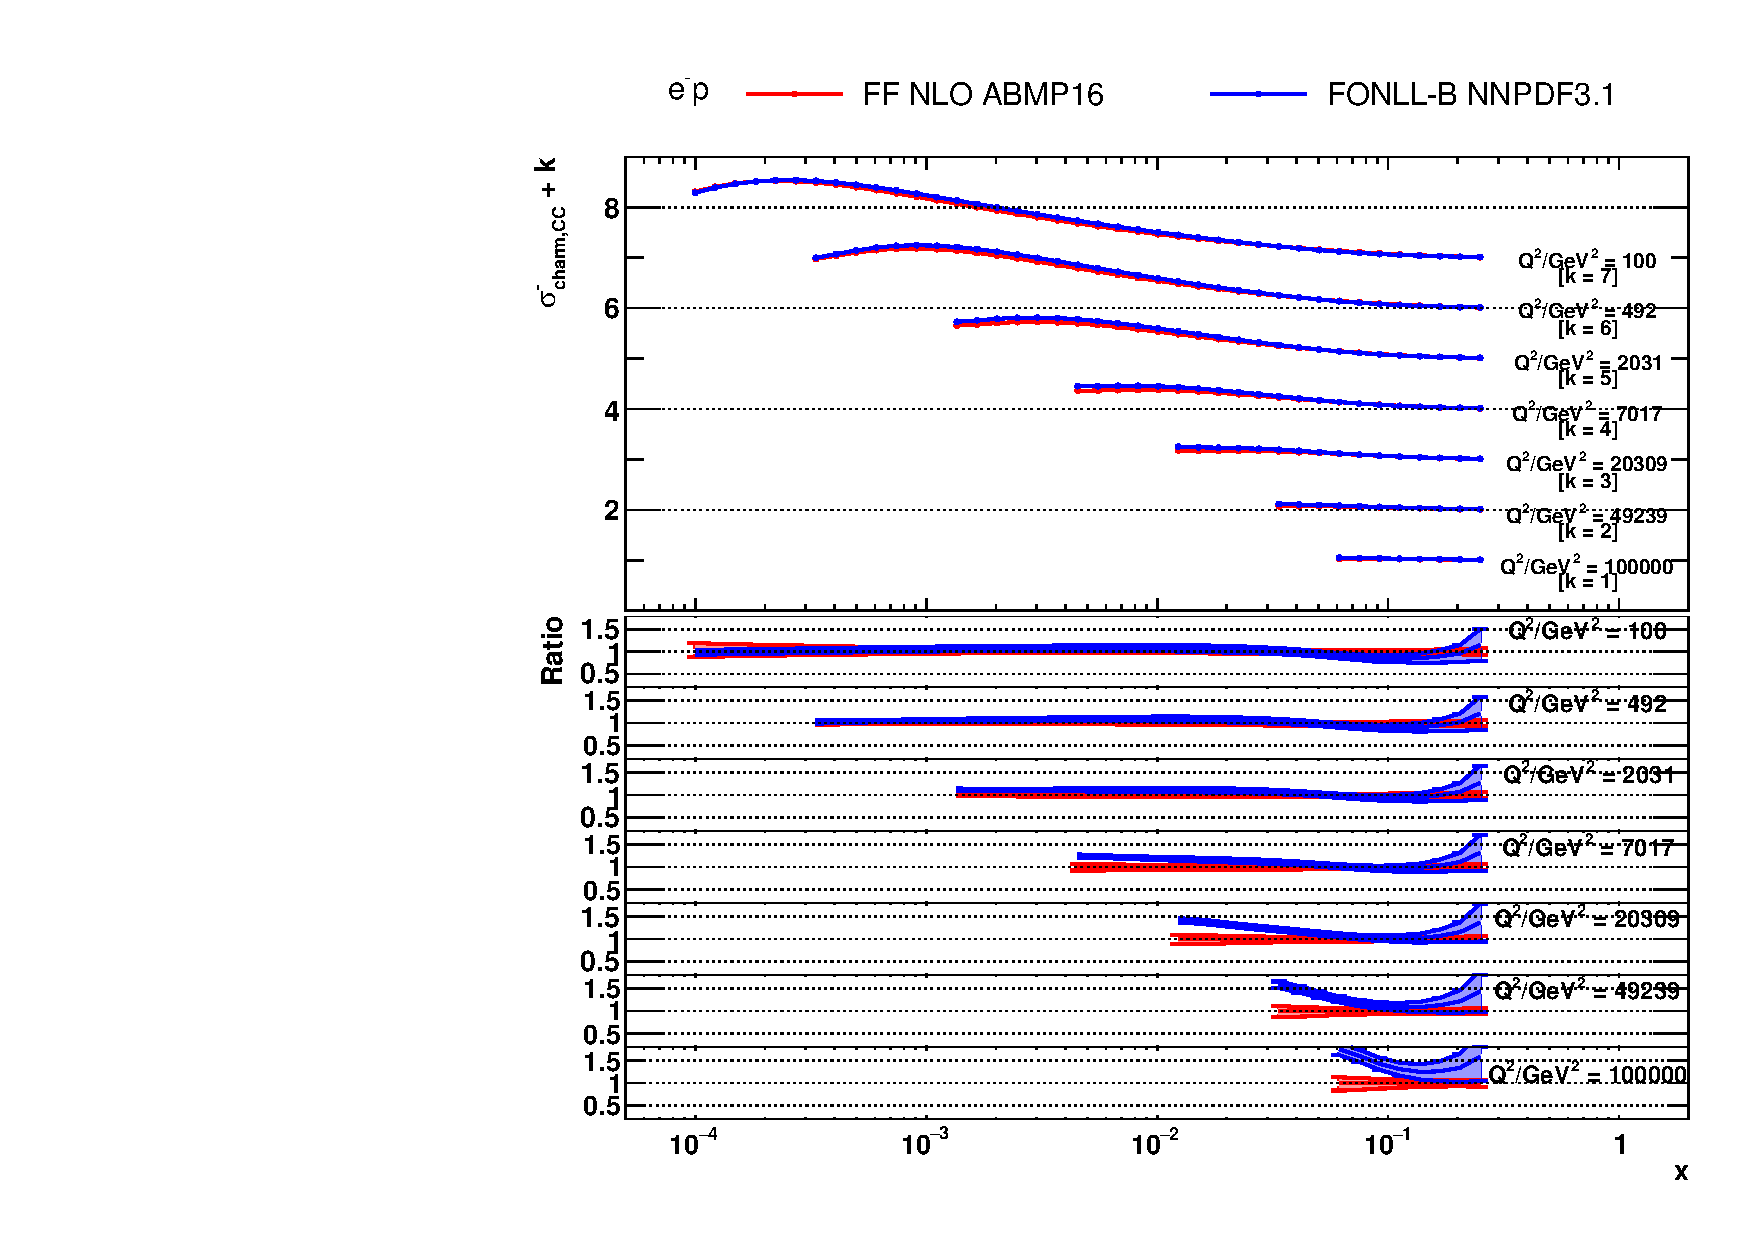
\includegraphics[width=0.50\textwidth]{pics/plots-110818/plot-sigmared-x-em.pdf}}}
    \caption{The theoretical predictions with their total uncertainties for charm CC production at the LHeC as a function of \xbj for different values of $Q^2$ calculated in the \ffns and \fonll schemes. The bottom panel display the theoretical predictions normalised to the nominal values of the \ffns predictions.}
    \label{fig:thpred-x}
\end{figure}

\begin{figure}
    \centering
    \centering{{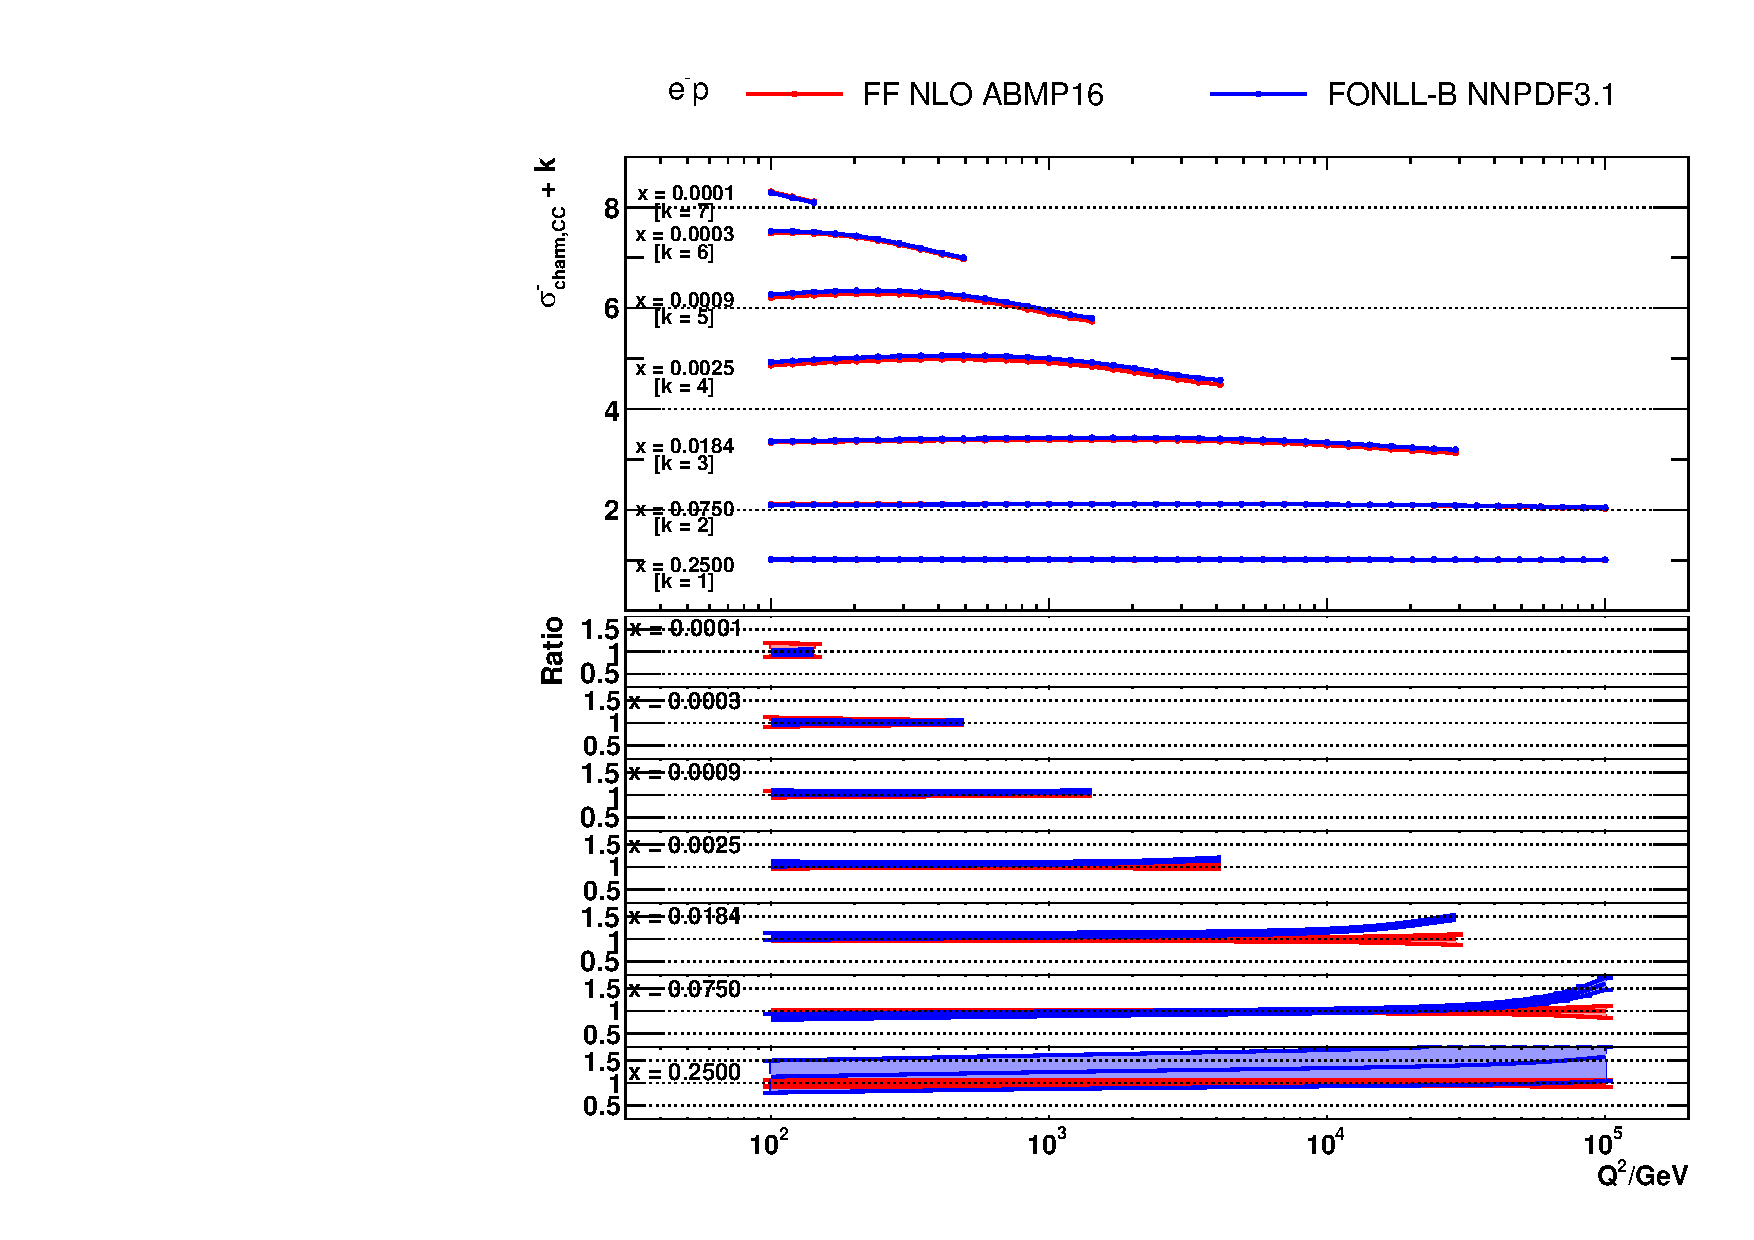
\includegraphics[width=0.50\textwidth]{pics/plots-110818/plot-sigmared-q2-em.pdf}}}
    \caption{The theoretical predictions with their total uncertainties for charm CC production at the LHeC as a function of $Q^2$ for different values of \xbj calculated in the \ffns and \fonll schemes. The bottom panel display the theoretical predictions normalised to the nominal values of the \ffns predictions.}
    \label{fig:thpred-q2}
\end{figure}

\begin{figure}
    \centering
    \centering{{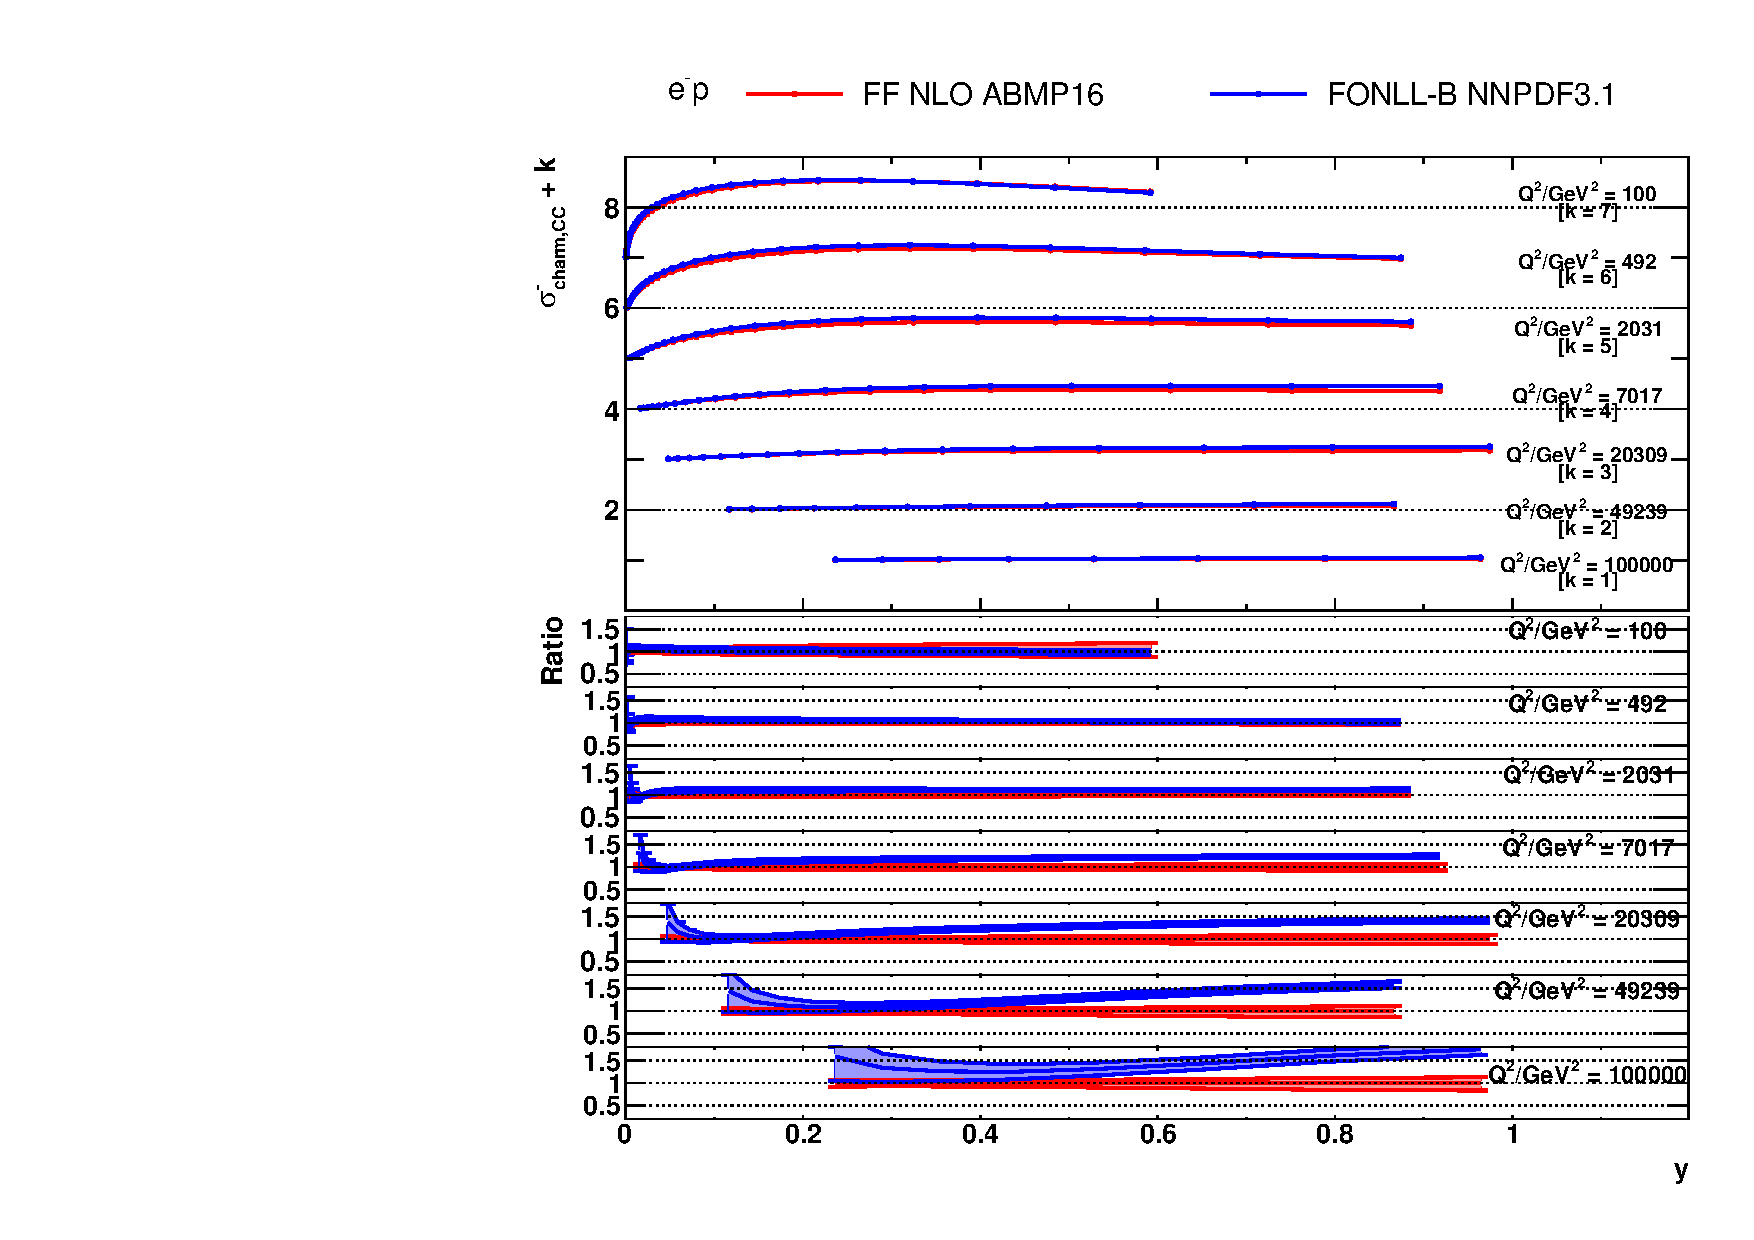
\includegraphics[width=0.50\textwidth]{pics/plots-110818/plot-sigmared-y-em.pdf}}}
    \caption{The theoretical predictions with their total uncertainties for charm CC production at the LHeC as a function of $y$ for different values of $Q^2$ calculated in the \ffns and \fonll schemes. The bottom panel display the theoretical predictions normalised to the nominal values of the \ffns predictions.}
    \label{fig:thpred-y}
\end{figure}

In Fig.~\ref{fig:thpred-q2-unc} the PDF and scale uncertainties of charm CC cross sections as a function of $Q^2$ for different values of \xbj calculated in the \ffns and \fonll schemes are shown. On average, in the \fonll scheme both the PDF and scale uncertainties exceed those in the \ffns scheme. Furthermore, Fig.~\ref{fig:thpred-q2-varmu} shows the impact of separate scale variations in the two schemes. In the \fonll scheme, the variation of $\mu_f$ has a much larger impact on the predictions than the variation of $\mu_r$, and thus it is dominant for the resulting scale uncertainties. {\bf [Valerio, could you please discuss more here?]} Only the simultaneous $\mu_f = \mu_r$ variation is available in the implementation of the \ffns scheme. 
%Overall, the scale variations in the \fonll scheme appears to be larger than those in the \ffns scheme.

\begin{figure*}
    \centering
    \centering{{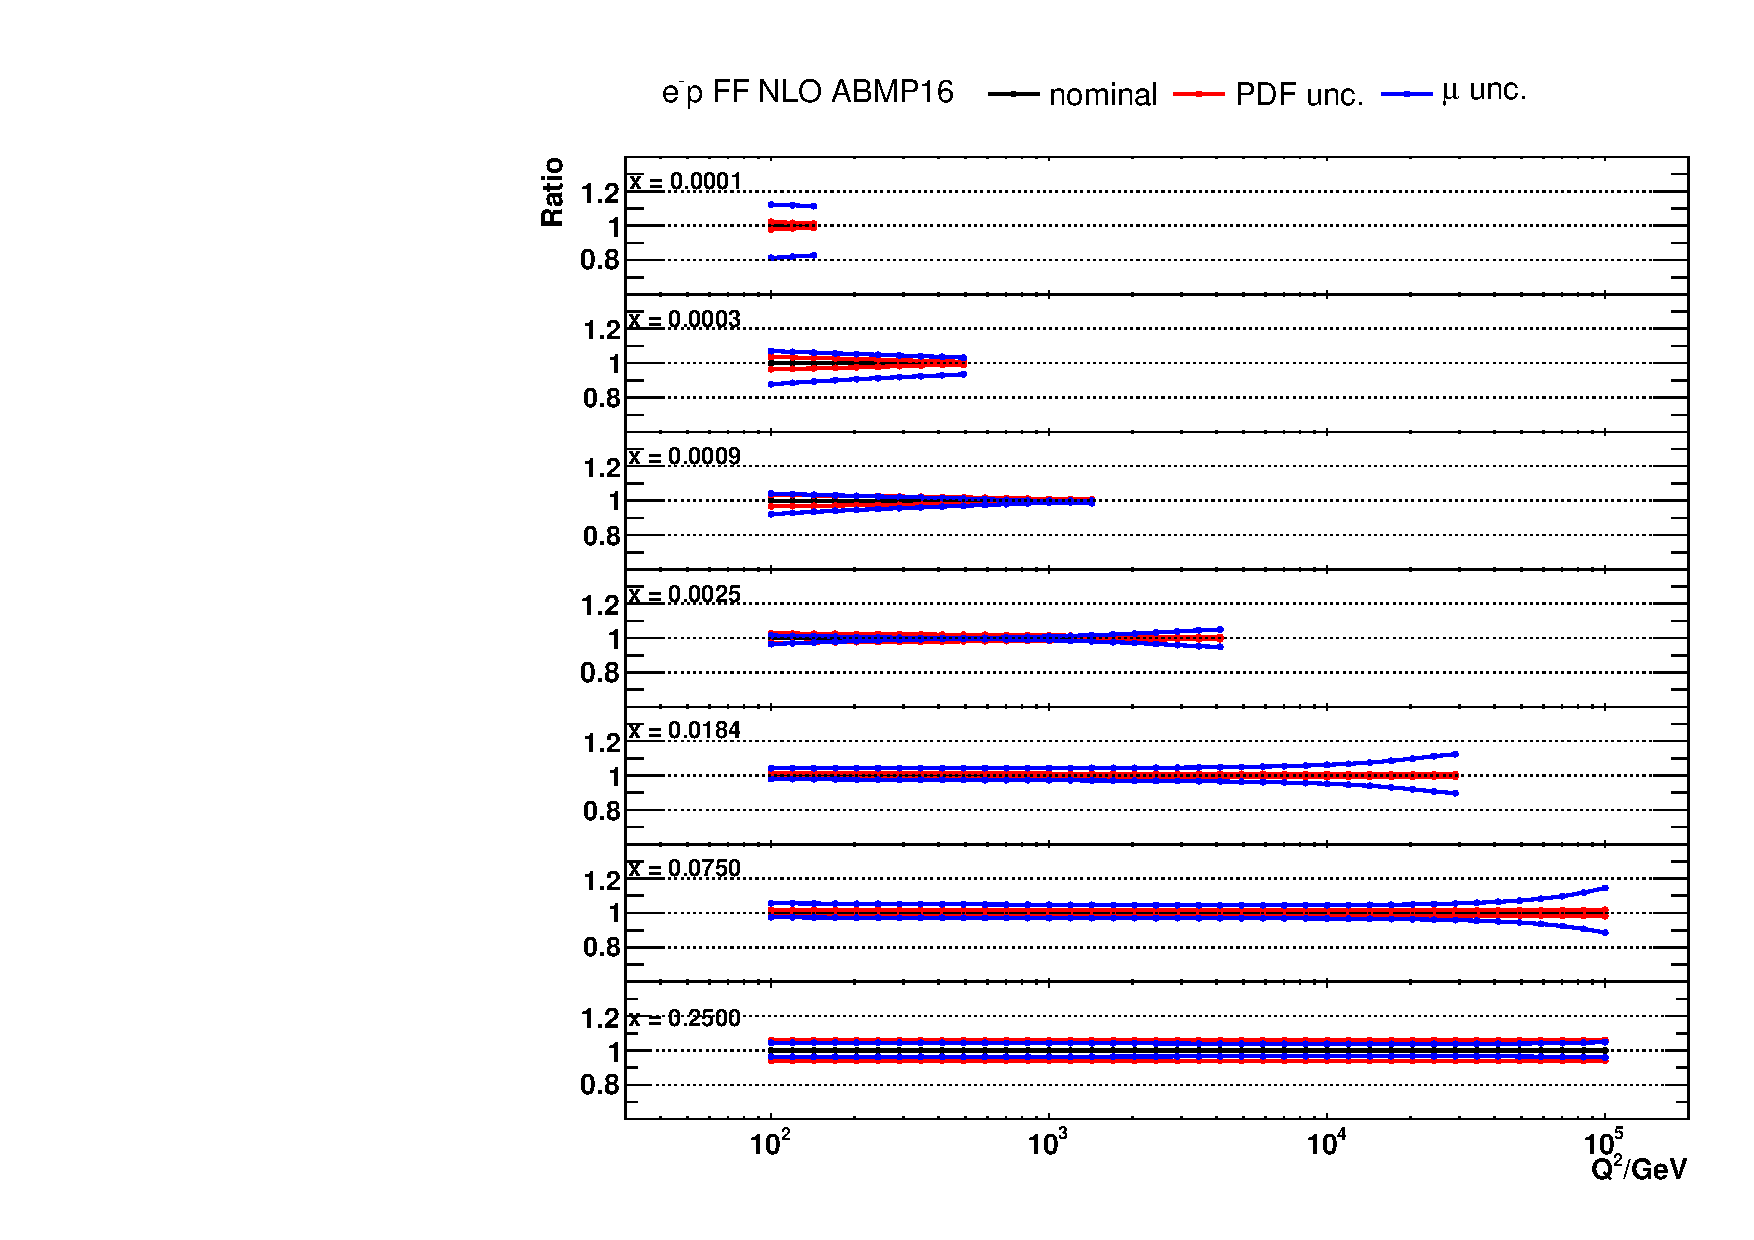
\includegraphics[width=0.49\textwidth]{pics/plots-130918/plot-unc-q2-em-FFABM.pdf}}}
    \centering{{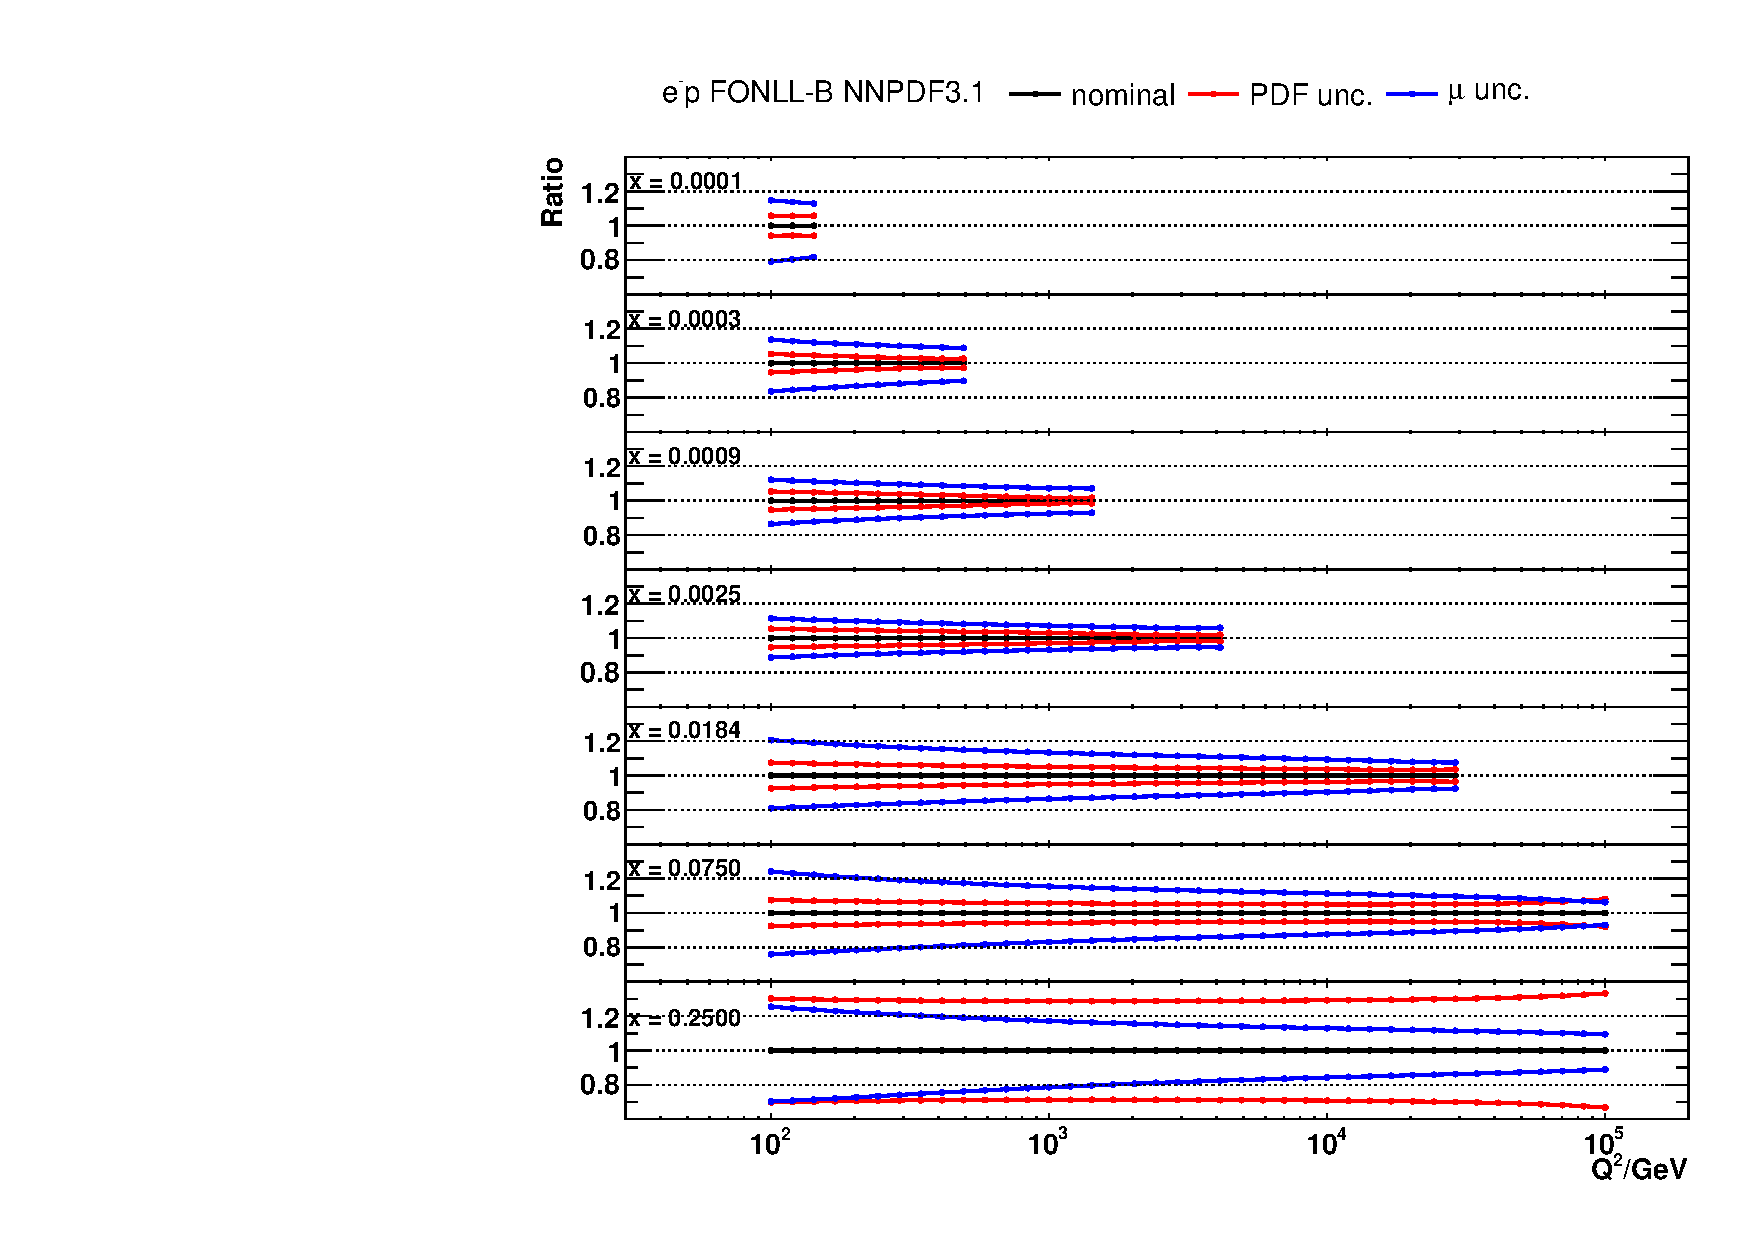
\includegraphics[width=0.49\textwidth]{pics/plots-130918/plot-unc-q2-em-FONLL.pdf}}}
    \caption{Relative theoretical uncertainties of charm CC predictions for the LHeC as a function of $Q^2$ for different values of \xbj calculated in the \ffns and \fonll schemes. The PDF and scale uncertainties are shown separately.}
    \label{fig:thpred-q2-unc}
\end{figure*}

\begin{figure*}
    \centering
    \centering{{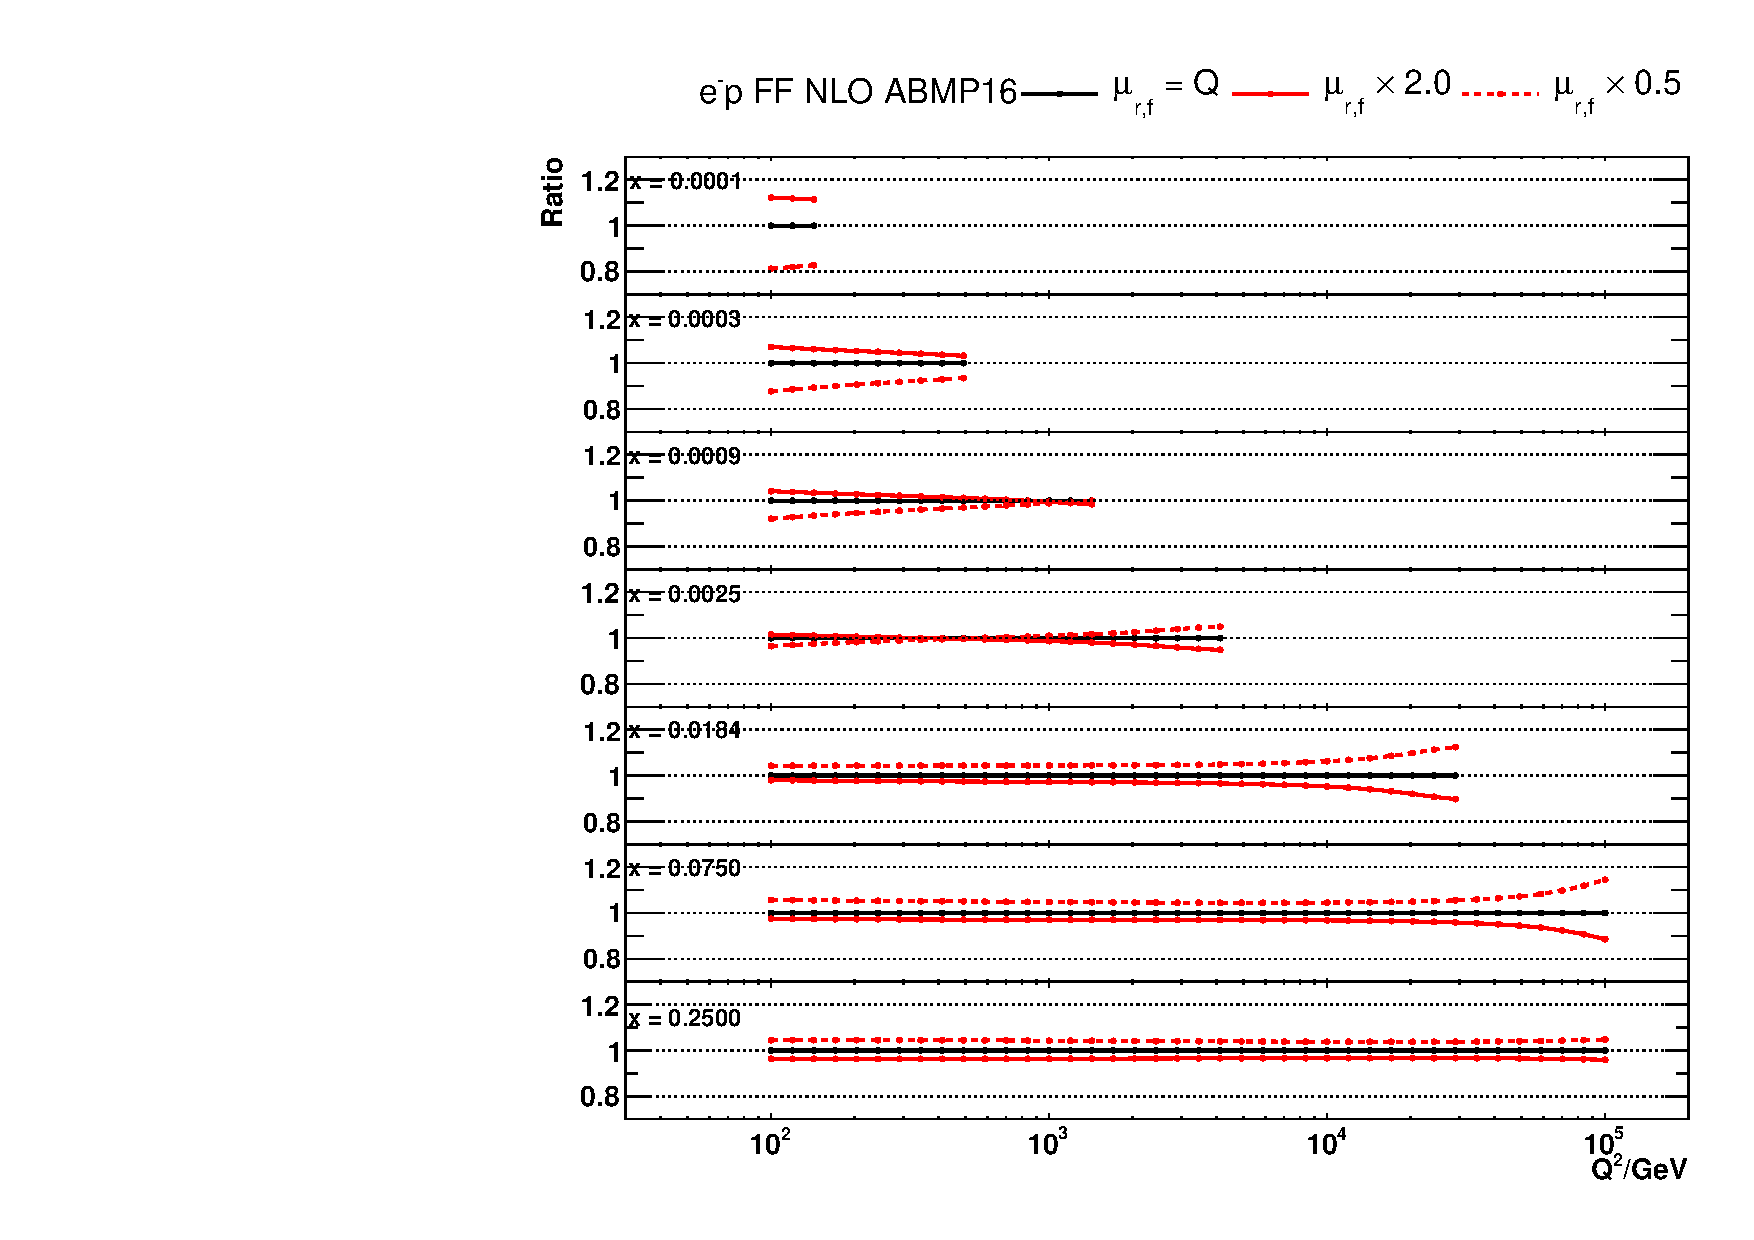
\includegraphics[width=0.49\textwidth]{pics/plots-130918/plot-varmu-q2-em-FFABM.pdf}}}
    \centering{{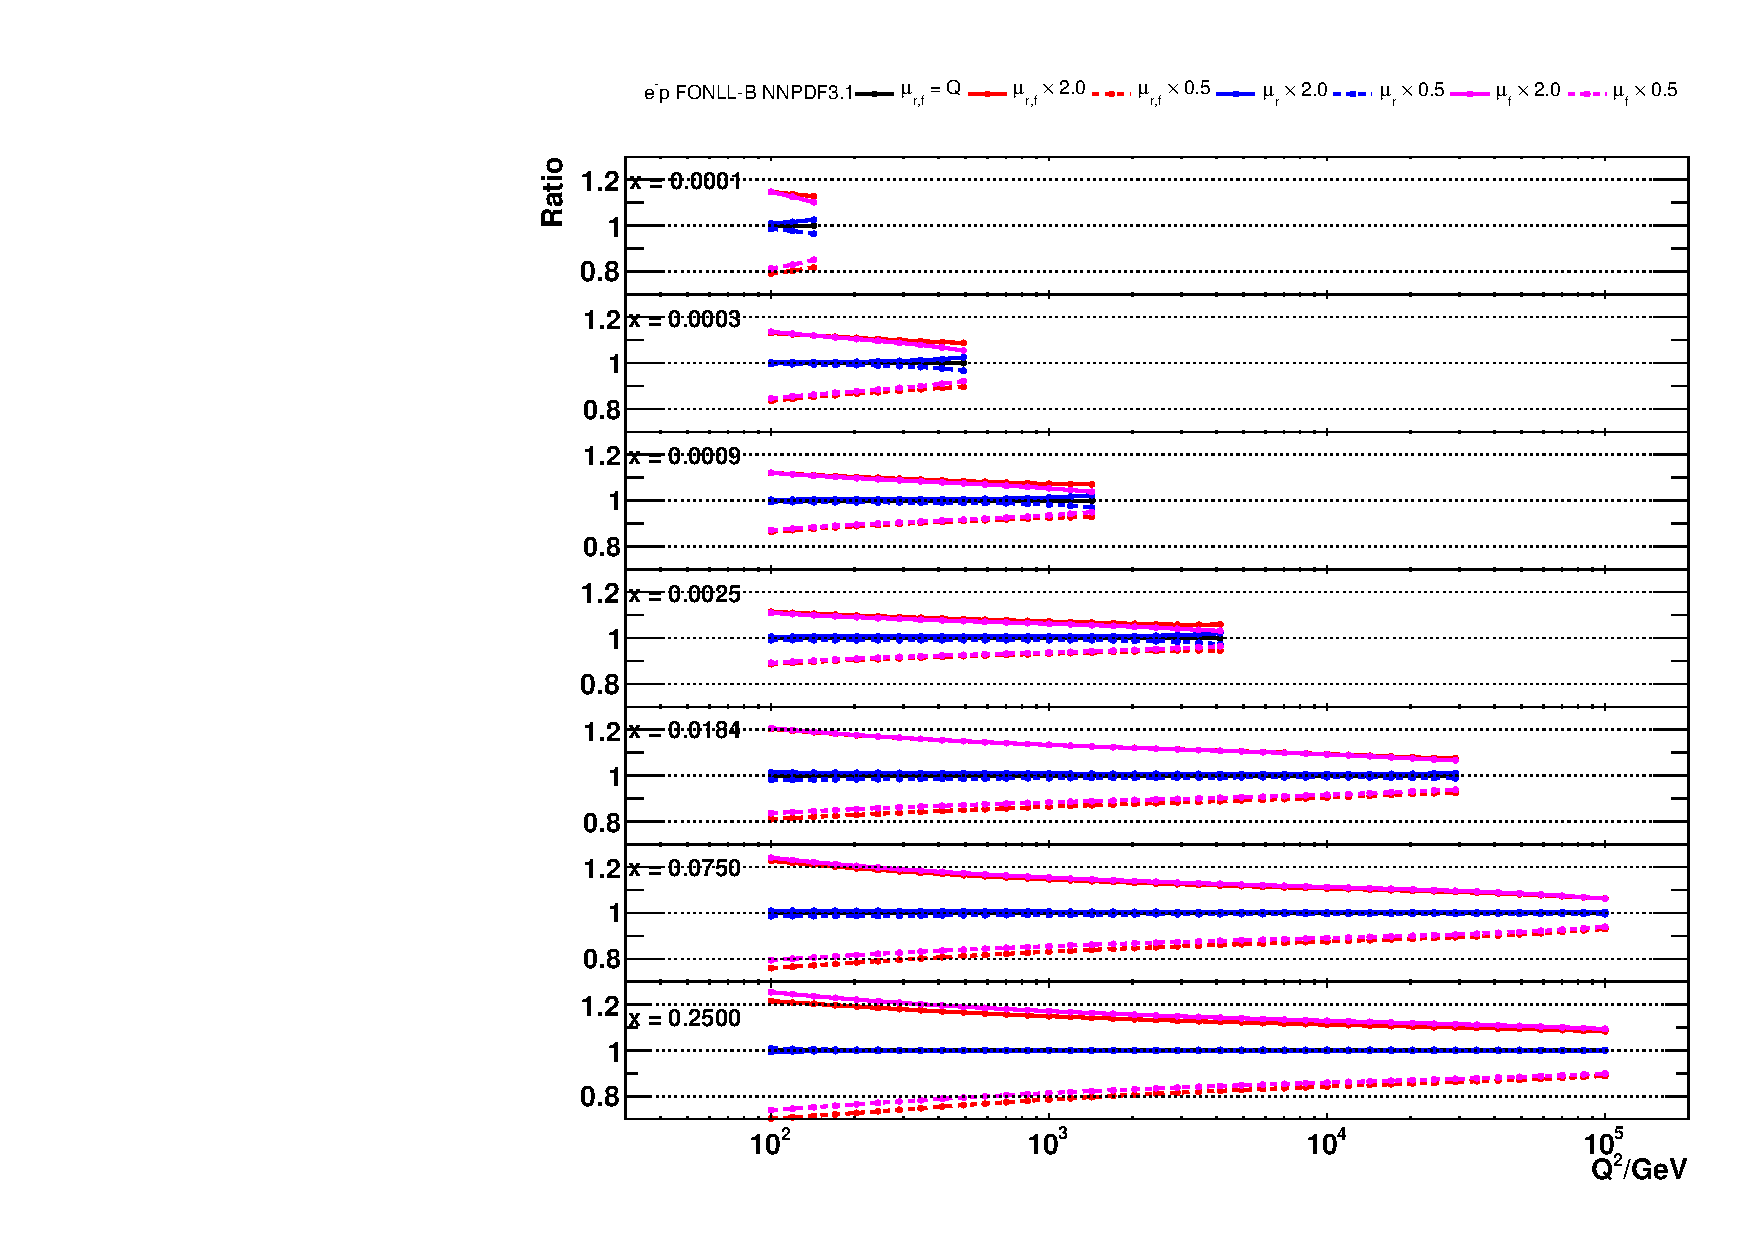
\includegraphics[width=0.49\textwidth]{pics/plots-130918/plot-varmu-q2-em-FONLL.pdf}}}
    \caption{The impact of separate scale variations on charm CC predictions for the LHeC as a function of $Q^2$ for different values of \xbj calculated in the \ffns and \fonll schemes.}
    \label{fig:thpred-q2-varmu}
\end{figure*}

To explore whether the differences between the two sets of theoretical predictions appear due to the different treatment of heavy quarks or due to different PDF sets, theoretical calculations in the \ffns and \fonll schemes are repeated with PDF sets extracted from the fit to the HERA DIS data~\cite{Abramowicz:2015mha}. The fit settings follow the HERAPDF2.0 analysis~\cite{Abramowicz:2015mha}. 
In this study, consistent conditions of the PDF extraction eliminate possible differences between the predictions for the LHeC arising from the dissimilarities of the \abmp and \nnpdf analysis. The obtained results are displayed in Figs.~\ref{fig:thpred-fit-y}--\ref{fig:thpred-fit-x}. The differences between the \ffns and \fonll schemes in these predictions are similar to the ones displayed in Figs.~\ref{fig:thpred-x}--\ref{fig:thpred-y} and prove that these differences arise due to the different treatment of heavy quarks in the two schemes.

Furthermore, the predictions in the \ffns and \ffnsb schemes calculated using the \ffthreea and \ffthreeb PDF sets are displayed in Figs.~\ref{fig:thpred-fit-y}--\ref{fig:thpred-fit-x}. Because of the similarities of the two HERAPDF2.0 PDF sets, the differences between the two sets of the predictions arise mainly due to the different treatment of heavy quarks in the two schemes. Remarkably, the differences between \ffns and \fonll predictions are similar to the ones between \ffns and \ffnsb, i.e.\ a larger part of these differences arise due to the different treatment of heavy quarks in $\alpha_s(\mu)$ running.
{\bf [TODO: Achim, could you please comment more here?]}


\begin{figure*}
    \centering
    \centering{{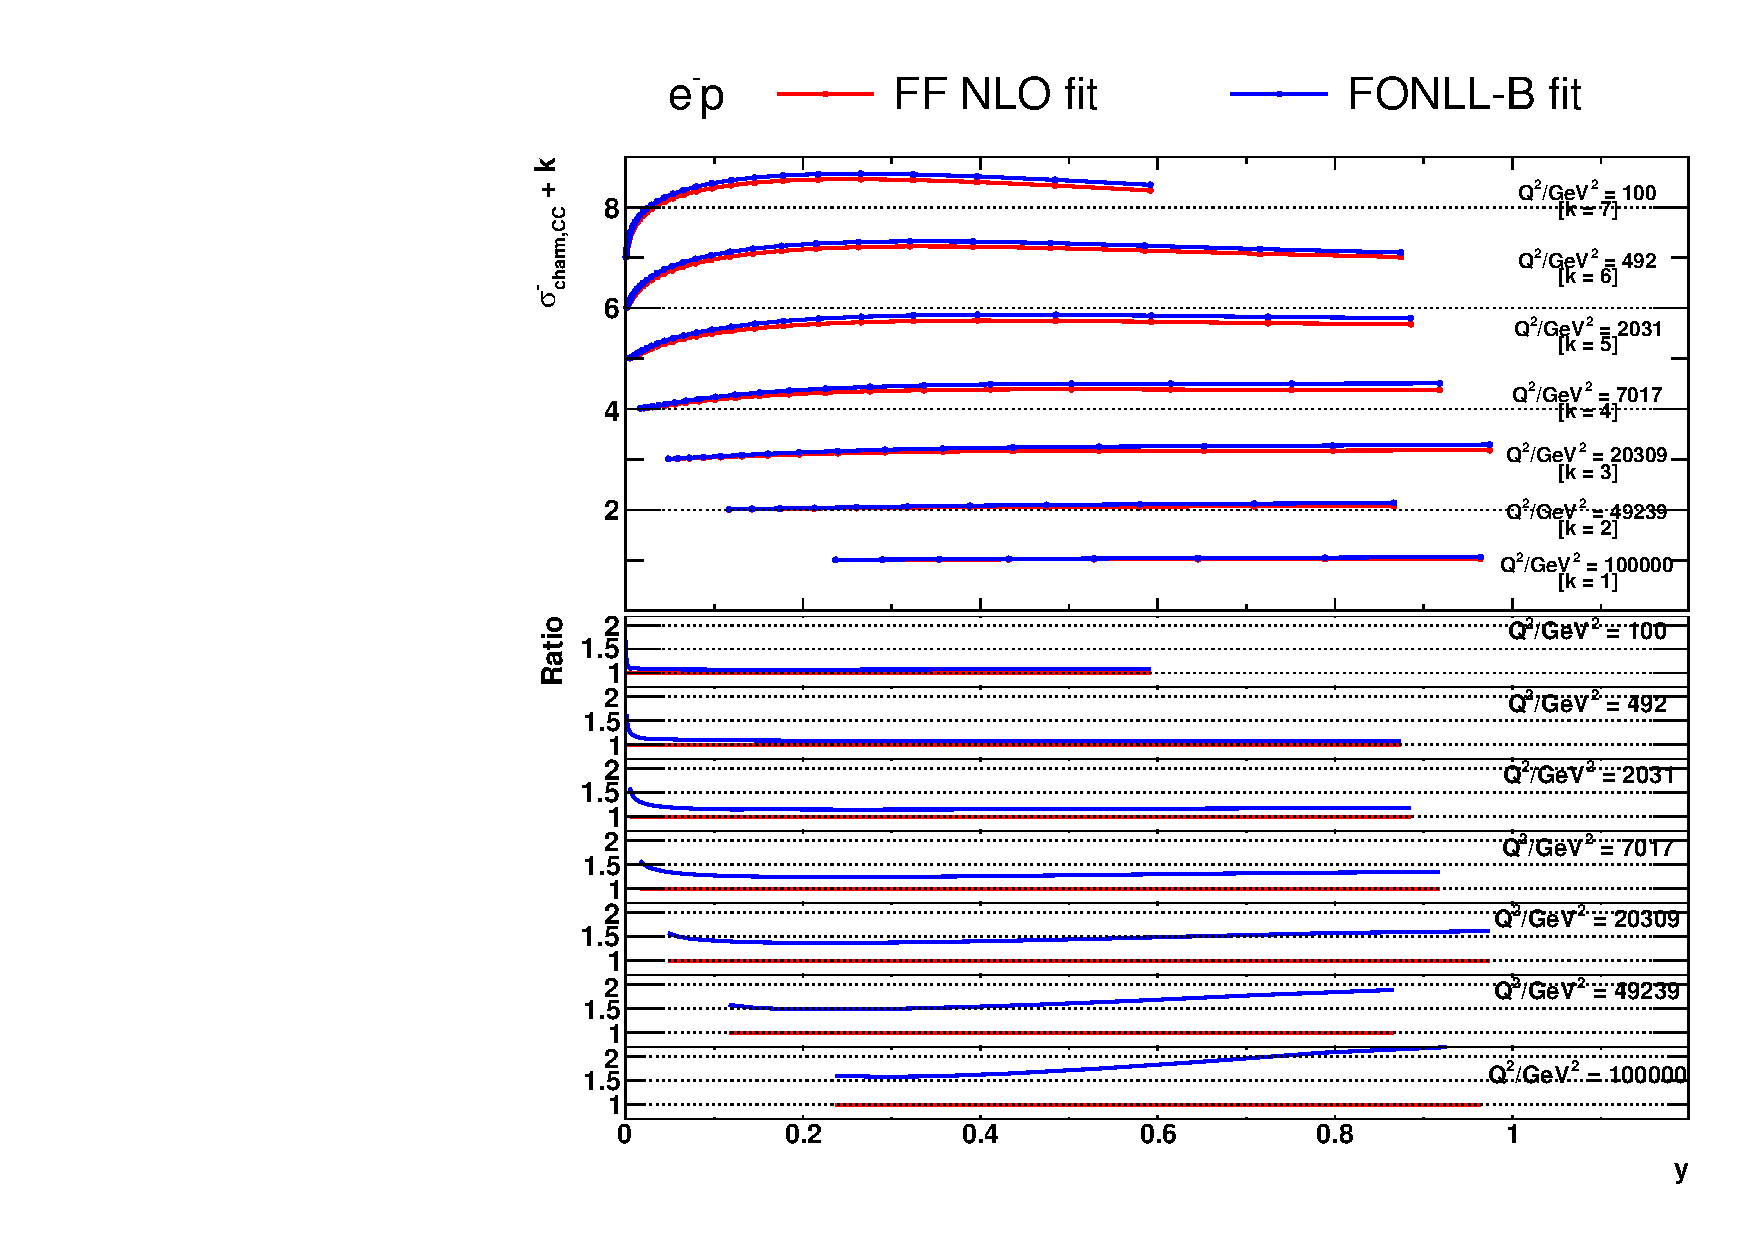
\includegraphics[width=0.49\textwidth]{pics/plots-191018/plot-fit-y-em.pdf}}}
    \centering{{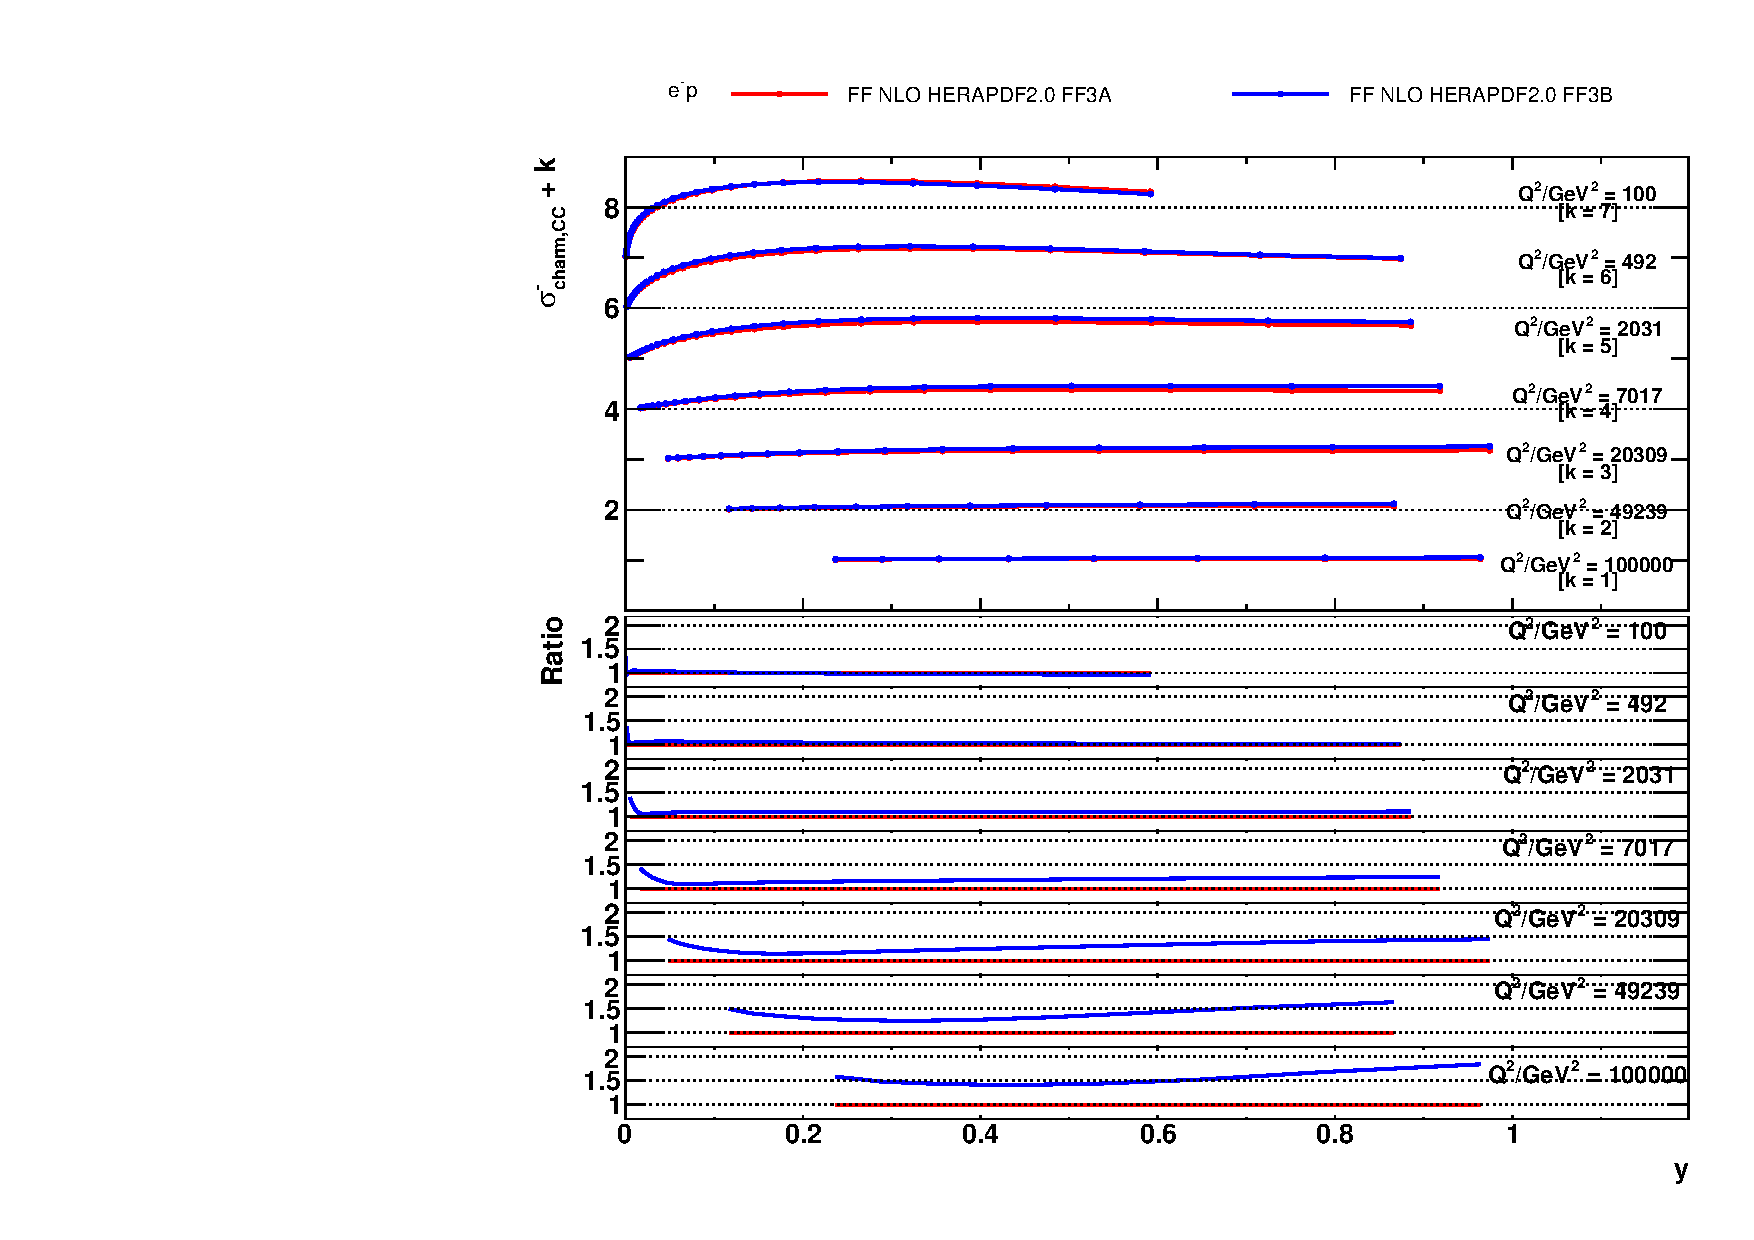
\includegraphics[width=0.49\textwidth]{pics/plots-191018/plot-FF3AB-y-em.pdf}}}
    \caption{(left) The theoretical predictions for charm CC production at the LHeC as a function of $y$ for different values of $Q^2$ obtained in the fit to the HERA data in the \ffns and \fonll schemes. The bottom panel display the theoretical predictions normalised to the nominal values of the \ffns predictions. (right) Same predictions but obtained in the \ffns and \ffnsb schemes using the \ffthreea and \ffthreeb sets, respectively. The bottom panel display the theoretical predictions normalised to the nominal values of the \ffnsb predictions.}
    \label{fig:thpred-fit-y}
\end{figure*}

\begin{figure*}
    \centering
    \centering{{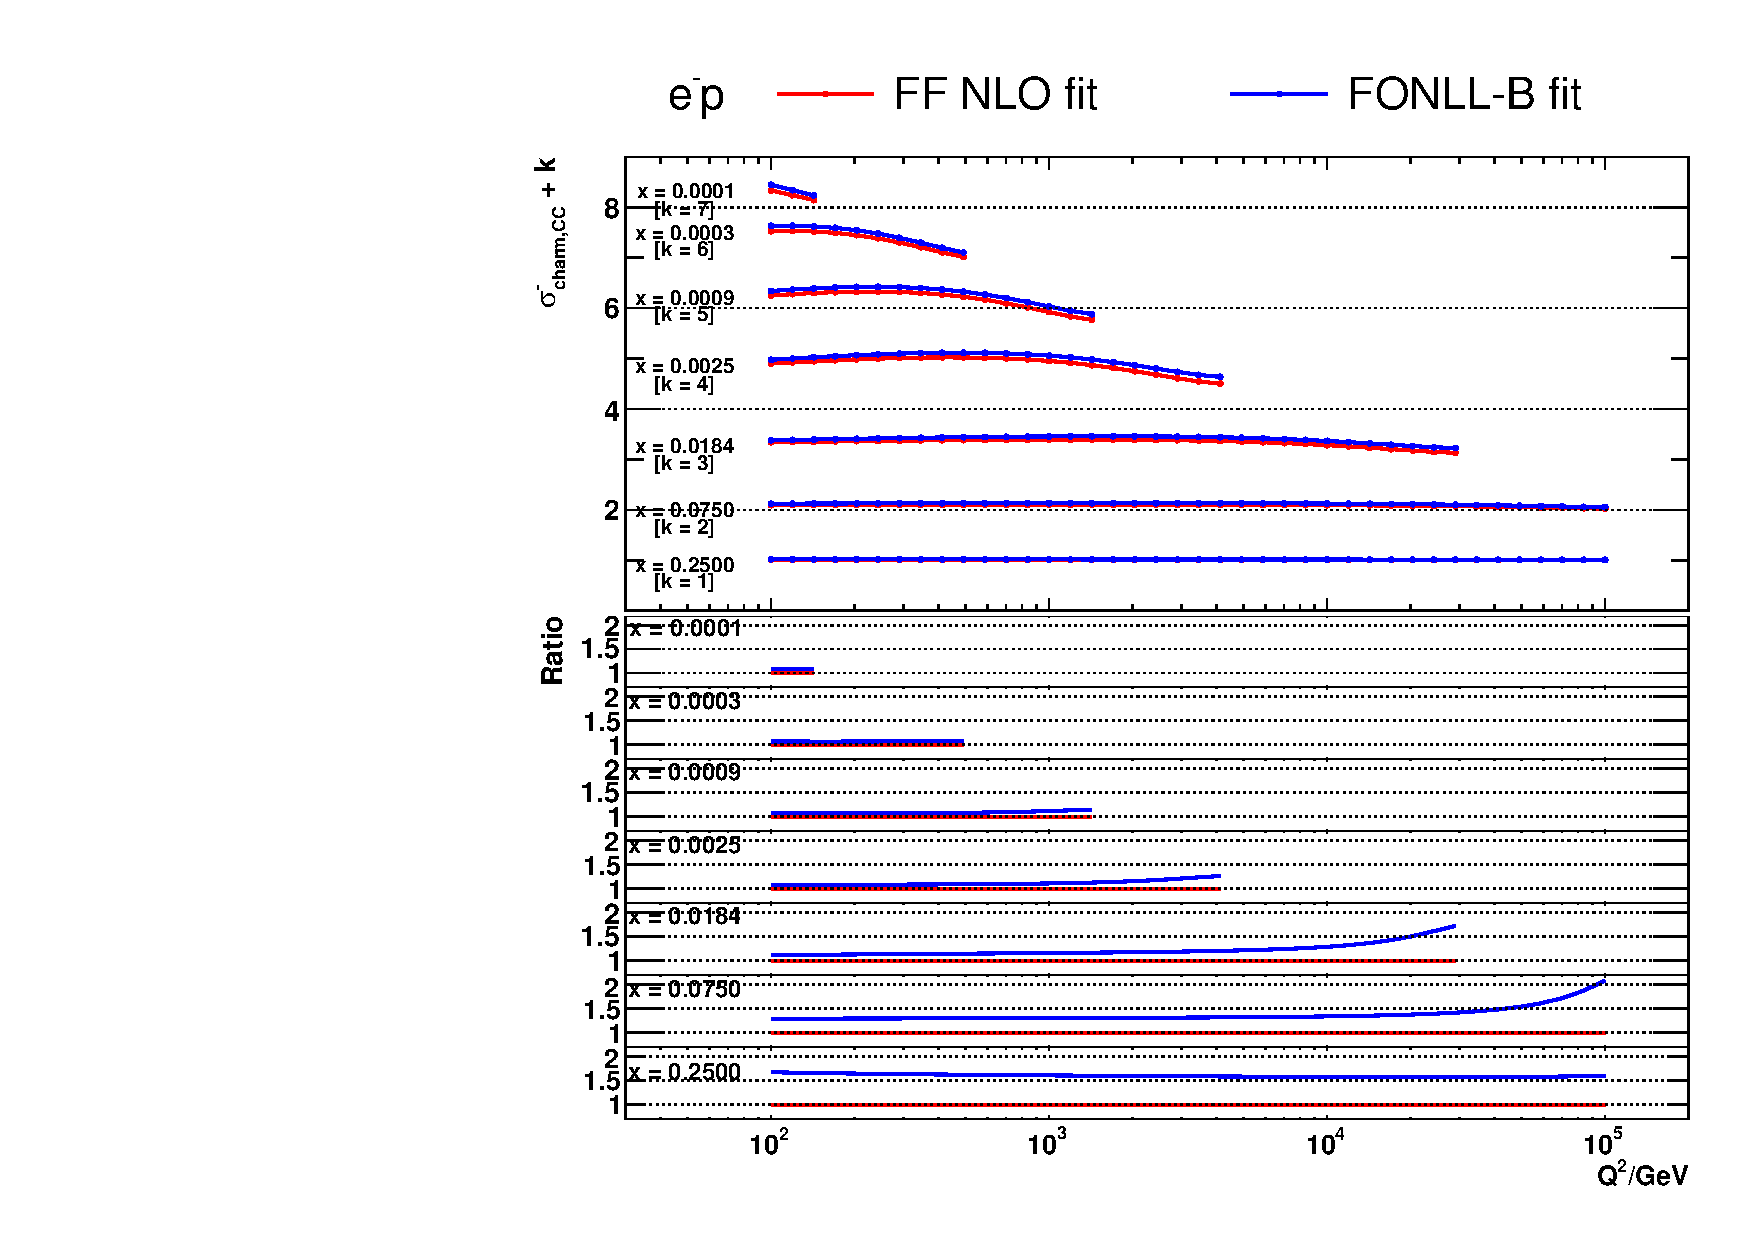
\includegraphics[width=0.49\textwidth]{pics/plots-191018/plot-fit-q2-em.pdf}}}
    \centering{{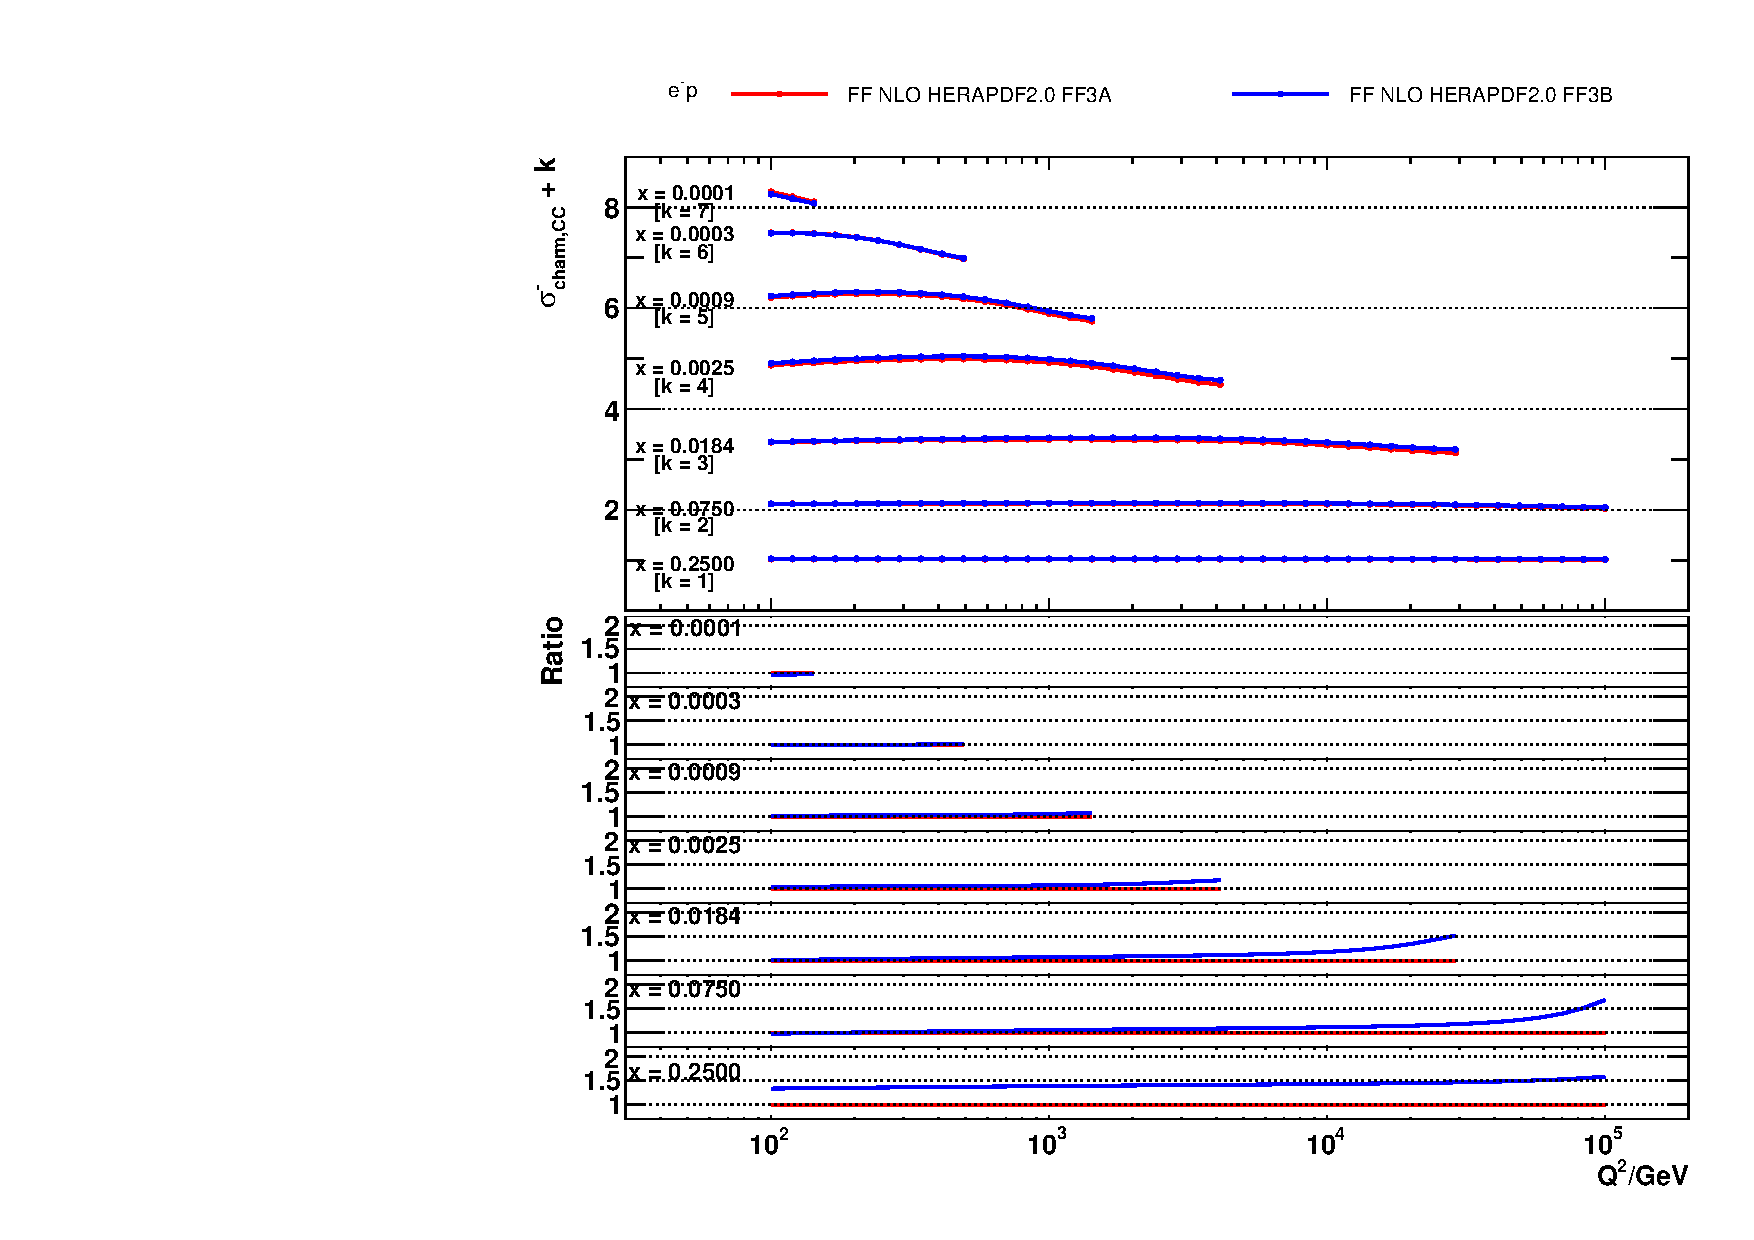
\includegraphics[width=0.49\textwidth]{pics/plots-191018/plot-FF3AB-q2-em.pdf}}}
    \caption{(left) The theoretical predictions for charm CC production at the LHeC as a function of $Q^2$ for different values of $\xbj$. See Fig.~\ref{fig:thpred-fit-y} for further details.}
    \label{fig:thpred-fit-q2}
\end{figure*}

\begin{figure*}
    \centering
    \centering{{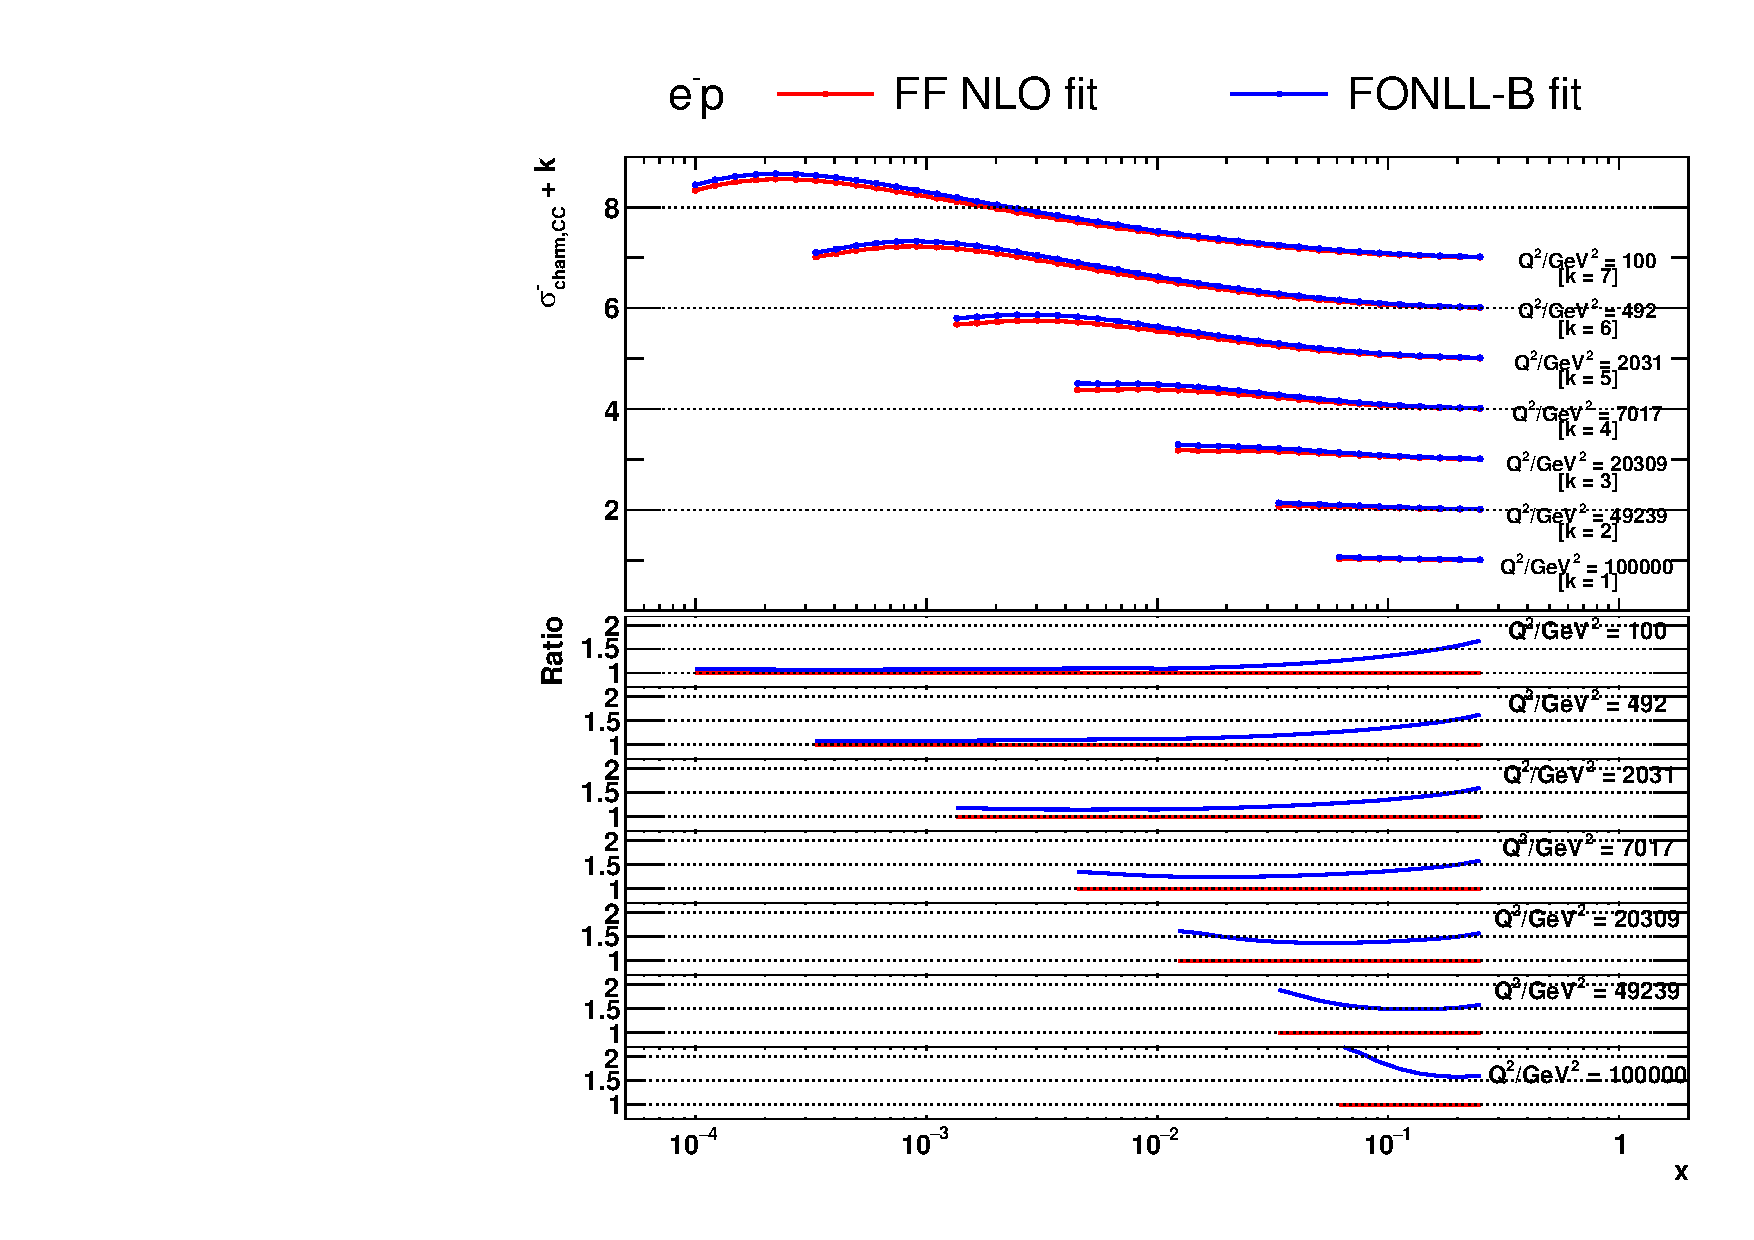
\includegraphics[width=0.49\textwidth]{pics/plots-191018/plot-fit-x-em.pdf}}}
    \centering{{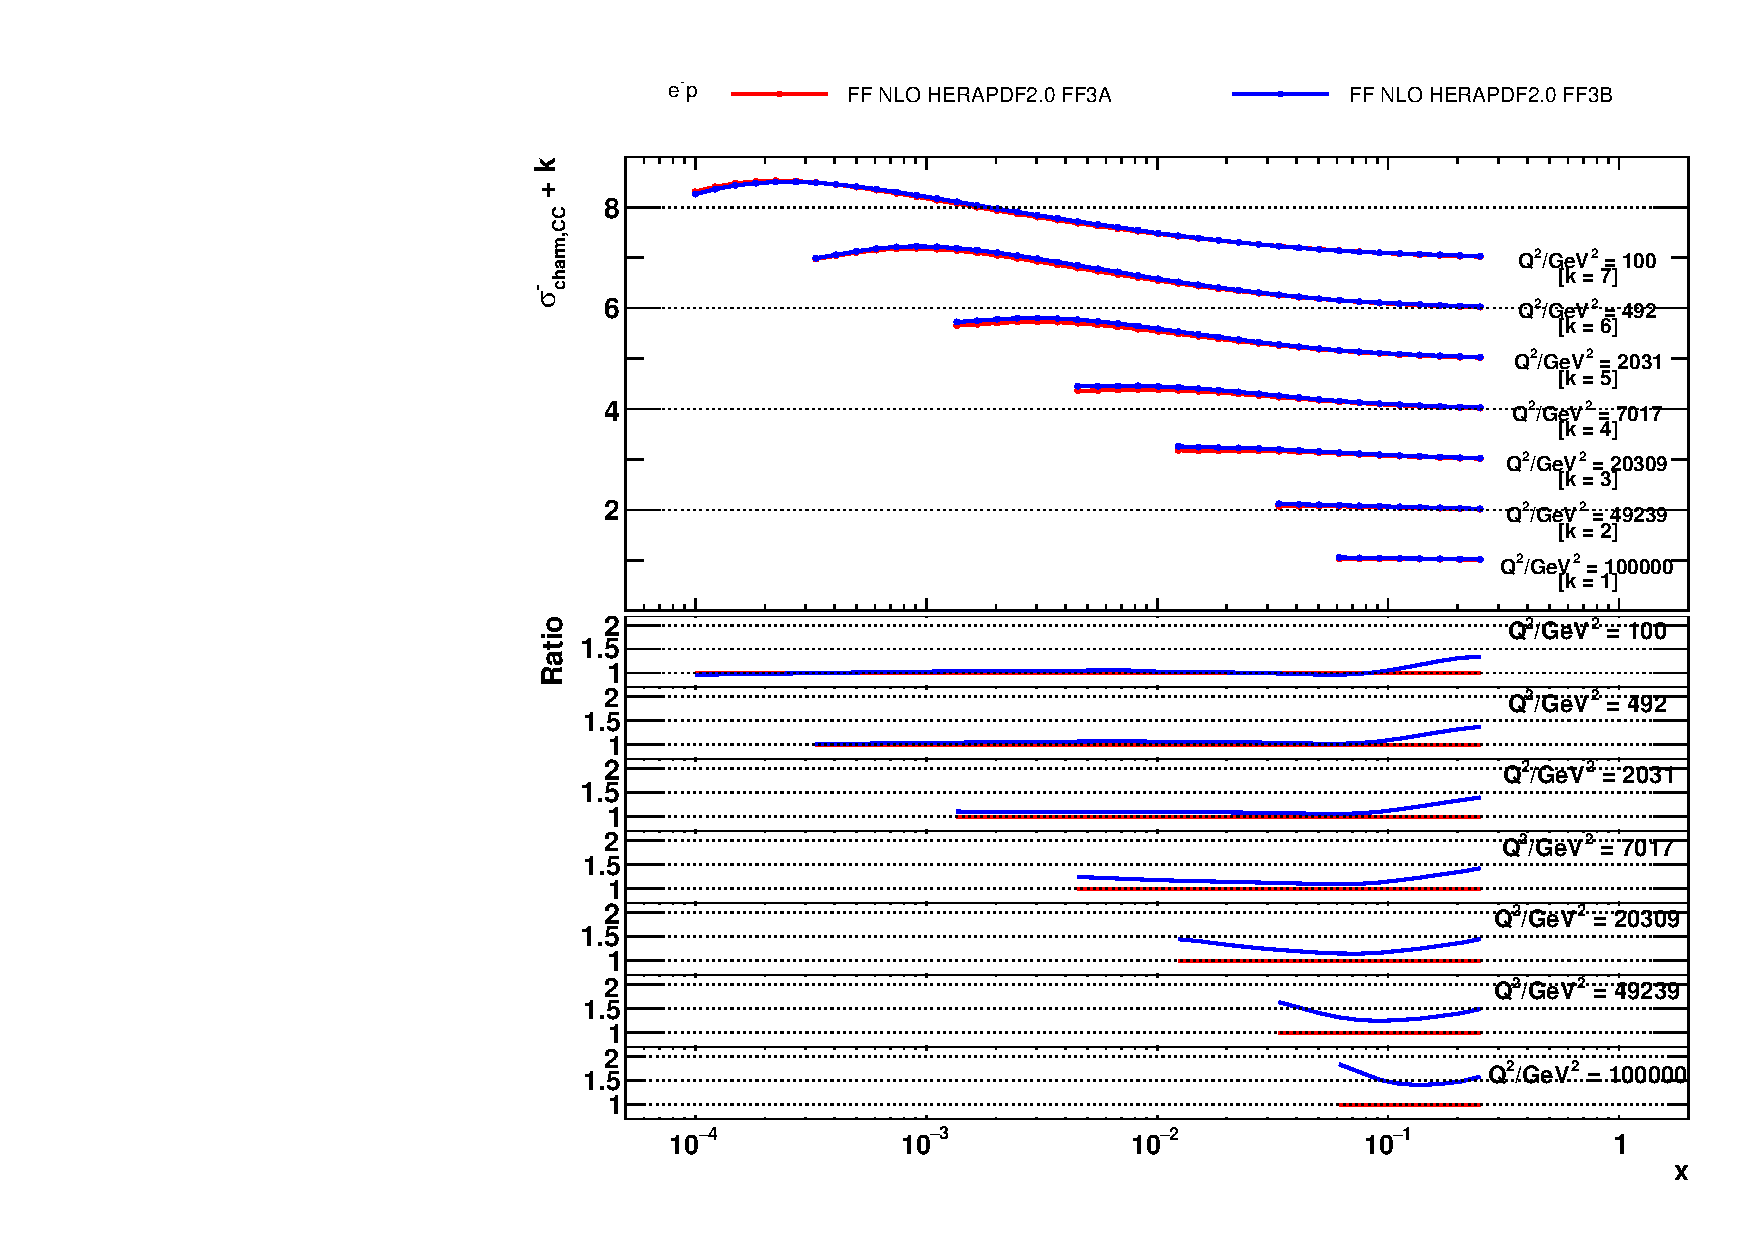
\includegraphics[width=0.49\textwidth]{pics/plots-191018/plot-FF3AB-x-em.pdf}}}
    \caption{(left) The theoretical predictions for charm CC production at the LHeC as a function of $Q^2$ for different values of $\xbj$. See Fig.~\ref{fig:thpred-fit-y} for further details.}
    \label{fig:thpred-fit-x}
\end{figure*}

Furthermore, to investigate the impact of the NNLO corrections available at $Q \gg m_c$ for the FFNS calculation, approximate NNLO predictions are obtained using the \abmp NNLO PDF set~\cite{Alekhin:2017kpj}. The results for the cross sections as a function of $Q^2$ for difference values of \xbj are shown in Fig.~\ref{fig:thpred-q2-nnlo}, where they are compared to the NLO FFNS predictions from Fig.~\ref{fig:thpred-q2}. The NNLO corrections do not exceed $10\%$ and thus do not cover the differences between the \ffns and \fonll theoretical predictions. Similar results are observed for cross sections as functions of other kinematic variables.

\begin{figure}
    \centering
    \centering{{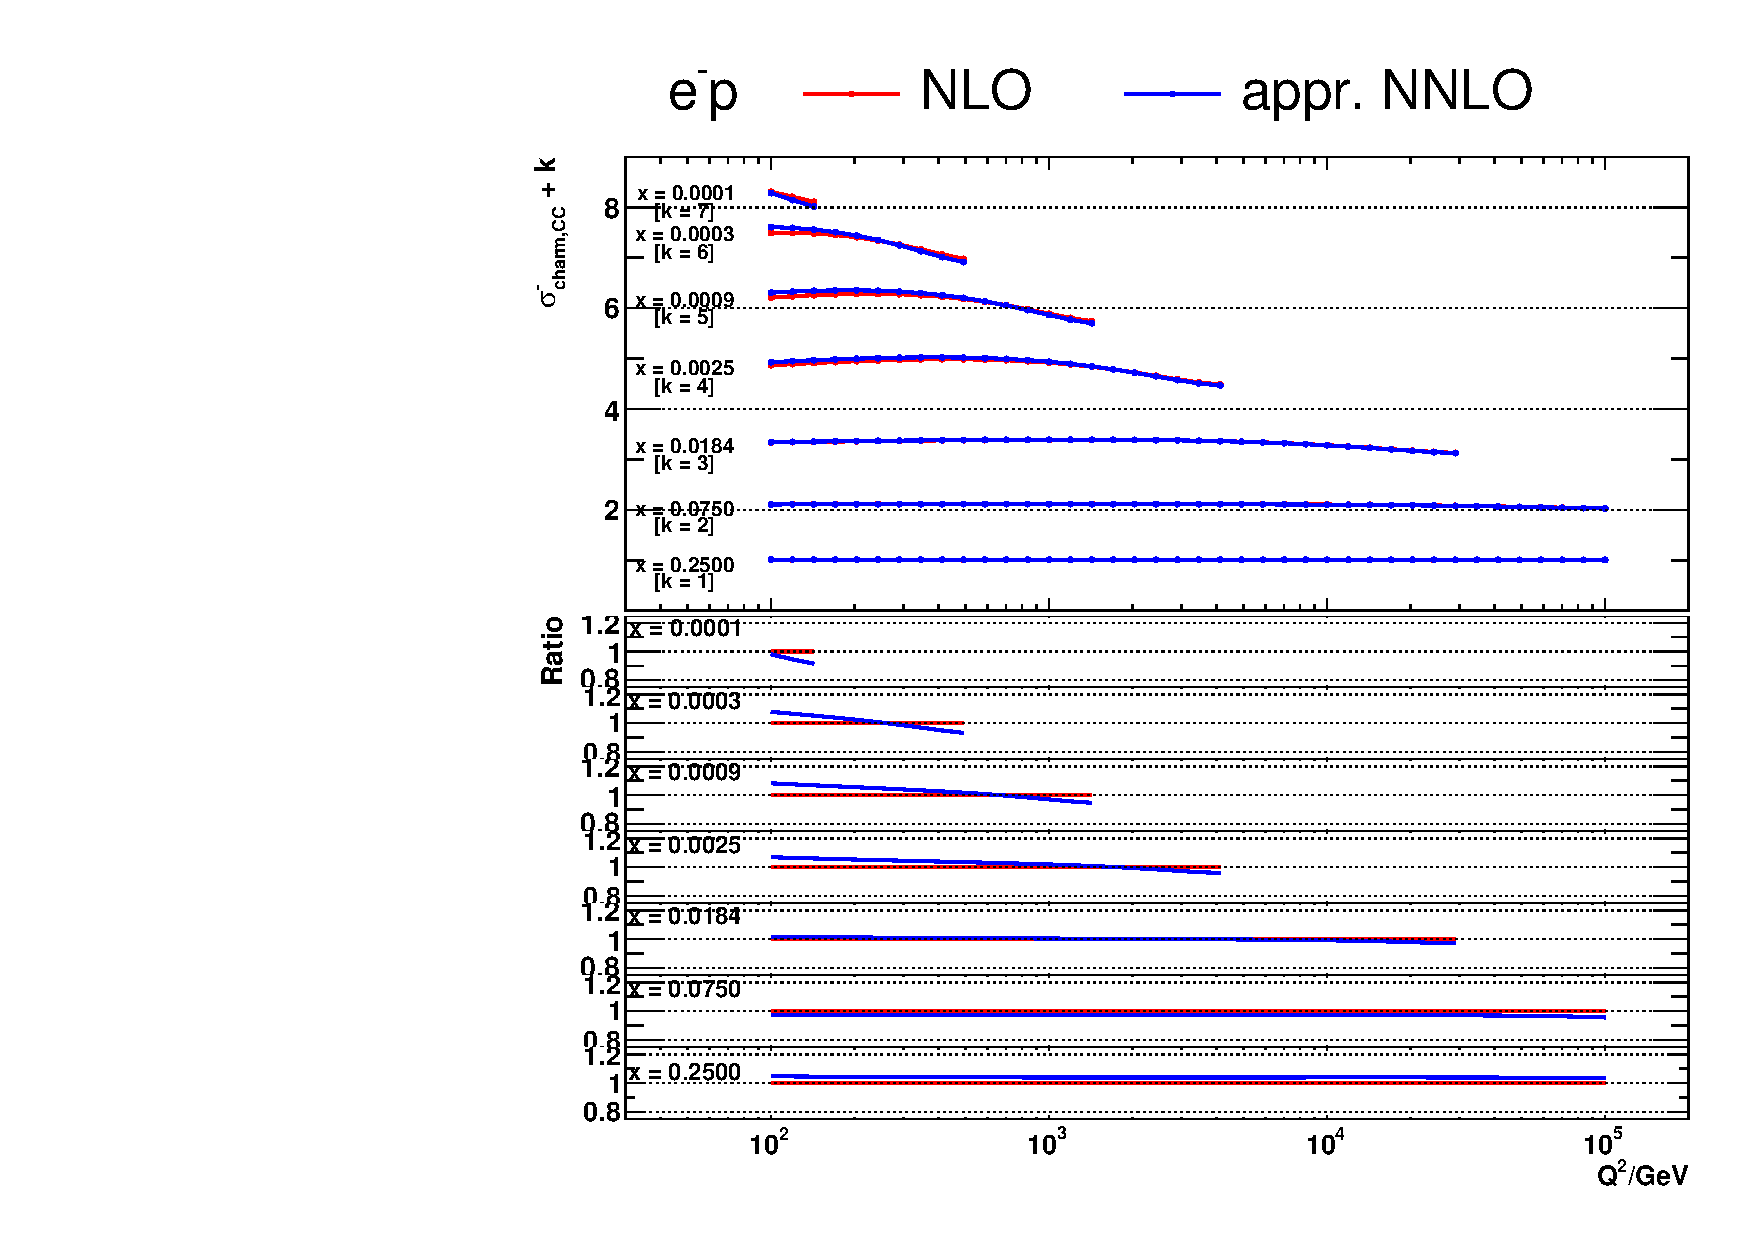
\includegraphics[width=0.50\textwidth]{pics/plots-130918/plot-FFABMnnlo-q2-em.pdf}}}
    \caption{The theoretical predictions with their total uncertainties for charm CC production at the LHeC as a function of $Q^2$ for different values of \xbj calculated in the \ffns scheme at NLO and approximate NNLO. The bottom panel display the theoretical predictions normalised to the nominal values of the \ffns NLO predictions.}
    \label{fig:thpred-q2-nnlo}
\end{figure}


\color{blue} %%%%%%%%%%%%%%%%%%%%%%%%%%%%%%%%%%%
To better understand the differences between the FFNS  and VFNS calculations, 
Fig.2*** which displays the cross section vs. $Q^2$ is particularly instructive. 
We see at low scales the FFNS and  VFNS results coincide. 
When the $\mu$ scale is below the charm threshold scale (typically taken to be $\sim m_c$)
the charm PDF vanishes and the FFNS and VFNS reduce to the same 
result.\footnote{Note that while the charm threshold scale $\mu_c$ is commonly 
set to the charm quark mass $m_c$, 
the choice of  $\mu_c$ is arbitrary and amounts to a 
renormalzation scheme choice~\cite{Bertone:2017ehk}.
}
%
For increasing scales, the VFNS resums the $\alpha_S \ln(\mu^2/m_c^2)$ contributions
via the DGLAP evolution equations and the FFNS and VFNS will slowly diverge logarithmically.
This behavior is observed in Fig.2*** and consistent with the characteristics demonstrated in 
Ref.~\cite{Kusina:2013slm}. 

More precisely, Ref.~\cite{Kusina:2013slm} used a matched set of $N_F=3$ and $N_F=5$ PDFs
to study the impact of the scheme choice at large scales. They found the resummed contributions 
in the VFNS yielded a larger cross section than the FFNS (the specific magnitude was $x$-dependent), and that for $Q$ scales more than a few times the quark mass, the differences due to scheme choice
exceeded the differences due to (estimated) higher order contributions~\cite{Kusina:2013slm}. 


\color{black} %%%%%%%%%%%%%%%%%%%%%%%%%%%%%%%%%%%



\subsection{Contributions from different partonic subprocesses}
\label{sec:thpred-partonic}

{\bf [perhaps this text would be more appropriate in an earlier theory section]}
The reduced charm CC production cross sections can be expressed as a linear combinations of the structure functions:
\begin{equation}
\begin{split}
    \sigma^{\pm}_{\text{charm,CC}} &= 0.5(Y_{+}F_2^{\pm} \mp Y_{-}xF_3^{\pm} - y^2F_L^{\pm}),\\
    Y_{\pm} &= 1 \pm (1-y)^2.
\end{split}
\end{equation}
In the simplified Quark Parton Model, where gluons are not present, the structure functions become:
\begin{equation}
\begin{split}
    F_2^{+} &= xD + x\overline{U}, \\
    F_2^{-} &= xU + x\overline{D},\\
    F_L &= 0,\\
    xF_3^{+} &= xD - x\overline{U}, \\
    xF_3^{-} &= xU - x\overline{D}.
\end{split}
\end{equation}
The terms $xU$, $xD$, $x\overline{U}$ and $x\overline{D}$ denote the sums of parton distributions for up-type and down-type quarks and anti-quarks, respectively. 
Below the $b$-quark mass threshold, these sums are related to the quark distributions as follows:
\begin{equation}
\begin{split}
 xU &= xu + xc , \\
 x\overline{U} &= x\overline{u} + x\overline{c} , \\
 xD &= xd + xs , \\
 x\overline{D} &= x\overline{d} + x\overline{s}.
\end{split}
\end{equation}
In the FFNS the charm quark density is zero.
In the phase space corners $y \to 0$ and $y \to 1$, the following asymptotics take place:
\begin{equation}
\begin{split}
 y \to 0: \sigma^{\pm}_{\text{charm,CC}} &= F_2^{\pm} = xD(x\overline{D}) + xU(x\overline{U}), \\
 y \to 1: \sigma^{\pm}_{\text{charm,CC}} &= 0.5(F_2^{\pm} \mp xF_3^{\pm}) = xU (x\overline{U}).
\label{eq:y01}
\end{split}
\end{equation}
Thus the contribution from the strange quark PDF is suppressed at high $y$.

Figures~\ref{fig:partonic-x}, \ref{fig:partonic-q2} and \ref{fig:partonic-y} show contributions from different partonic subprocesses for charm CC production cross sections in the \ffns and \fonll schemes as a function of \xbj for different values of $Q^2$, as a function of $Q^2$ for different values of \xbj, and as a function of $y$ for different values of $Q^2$, respectively.
In both scheme, the strange quark PDF contributes only about $50\%$ to total charm CC production. In particular, at high $y$ its contribution drops to zero in favor of the gluon or charm quark PDF (see Fig.~\ref{fig:partonic-y} and Eq.~\ref{eq:y01}). Similar phenomena (although less pronounced) is observed at low \xbj and/or high $Q^2$. In these phase space regions, the dominant contributions to the cross sections are the gluon PDF (in the FFNS) or the charm quark PDF (in the VFNS). Remarkably, these contributions as functions of $Q^2$, \xbj and $y$ behave qualitatively very similar in the FFNS and VFNS.

\begin{figure*}
    \centering
    \centering{{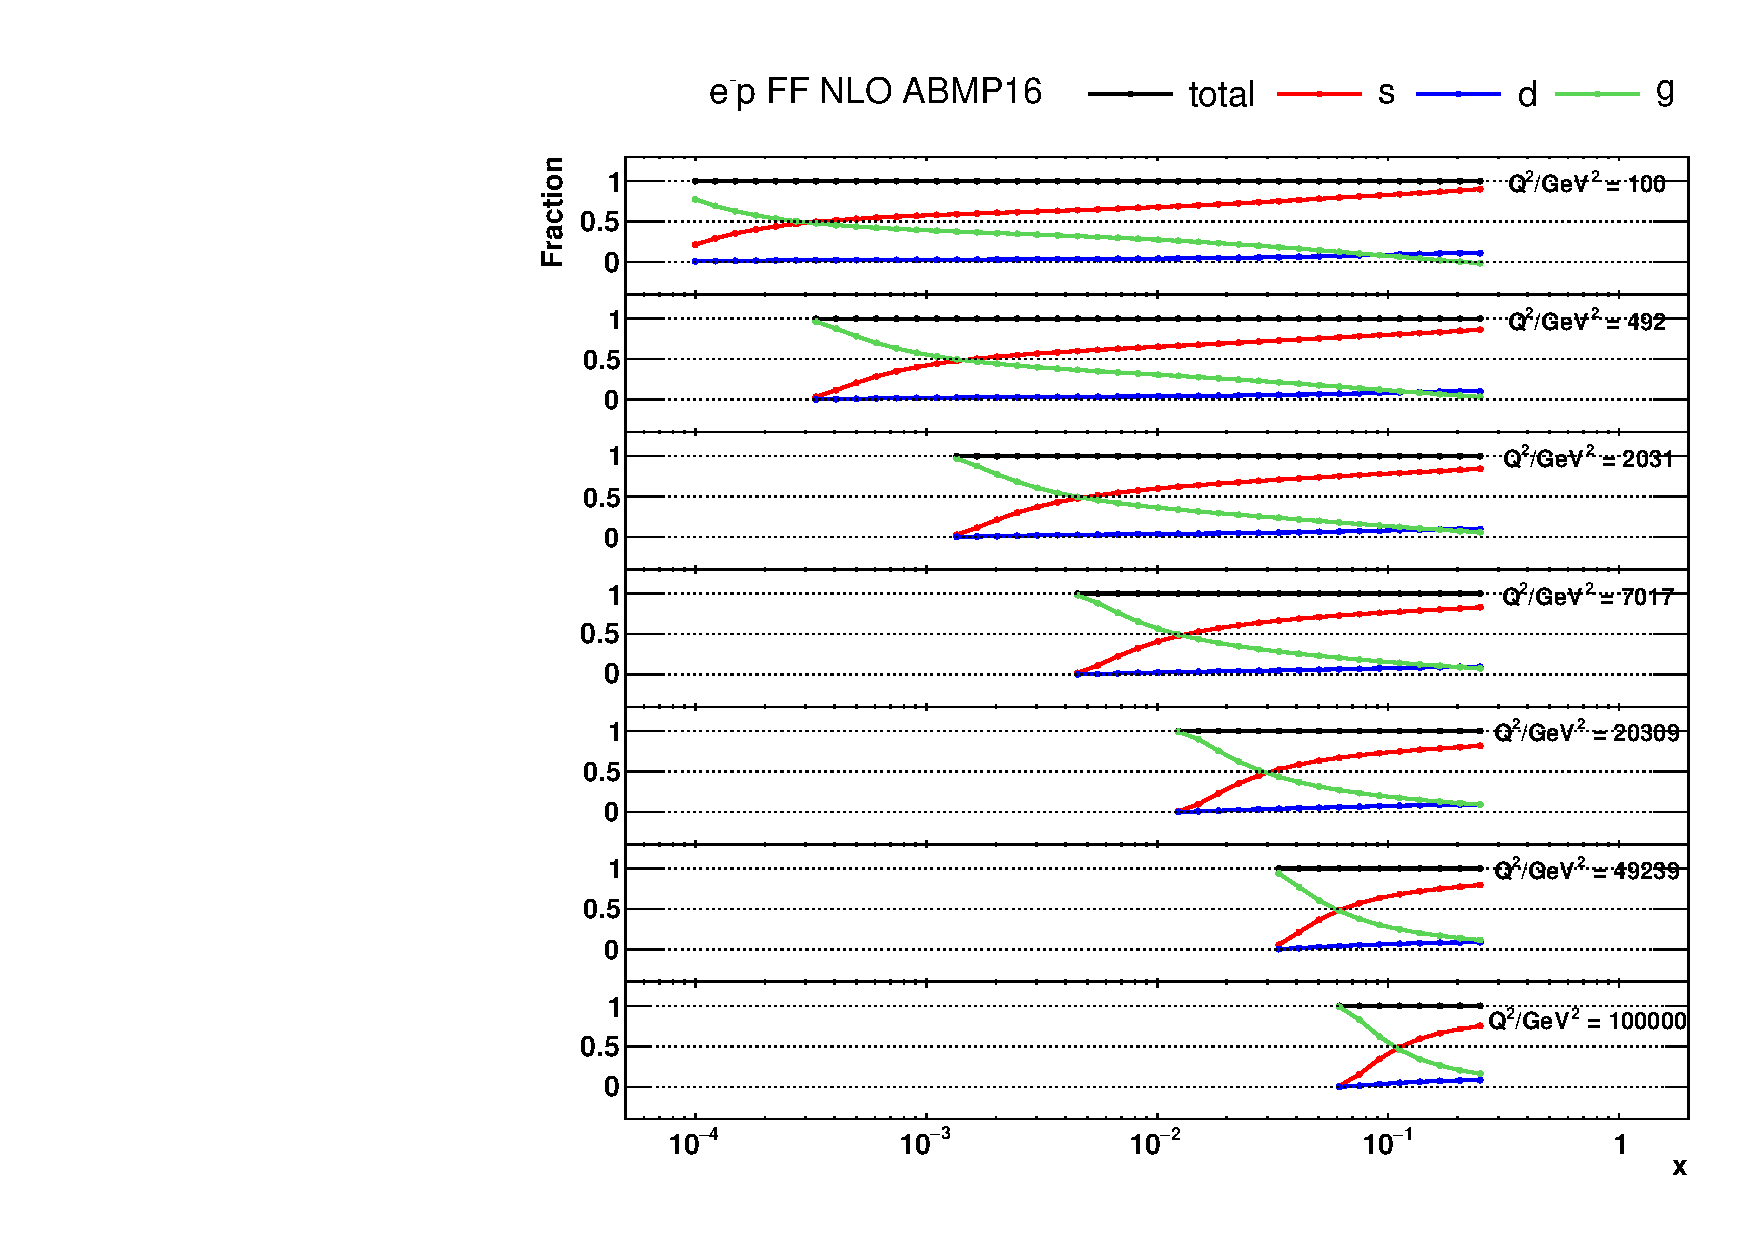
\includegraphics[width=0.49\textwidth]{pics/plots-110818/plot-parton-x-em-FFABM.pdf}}}
    \centering{{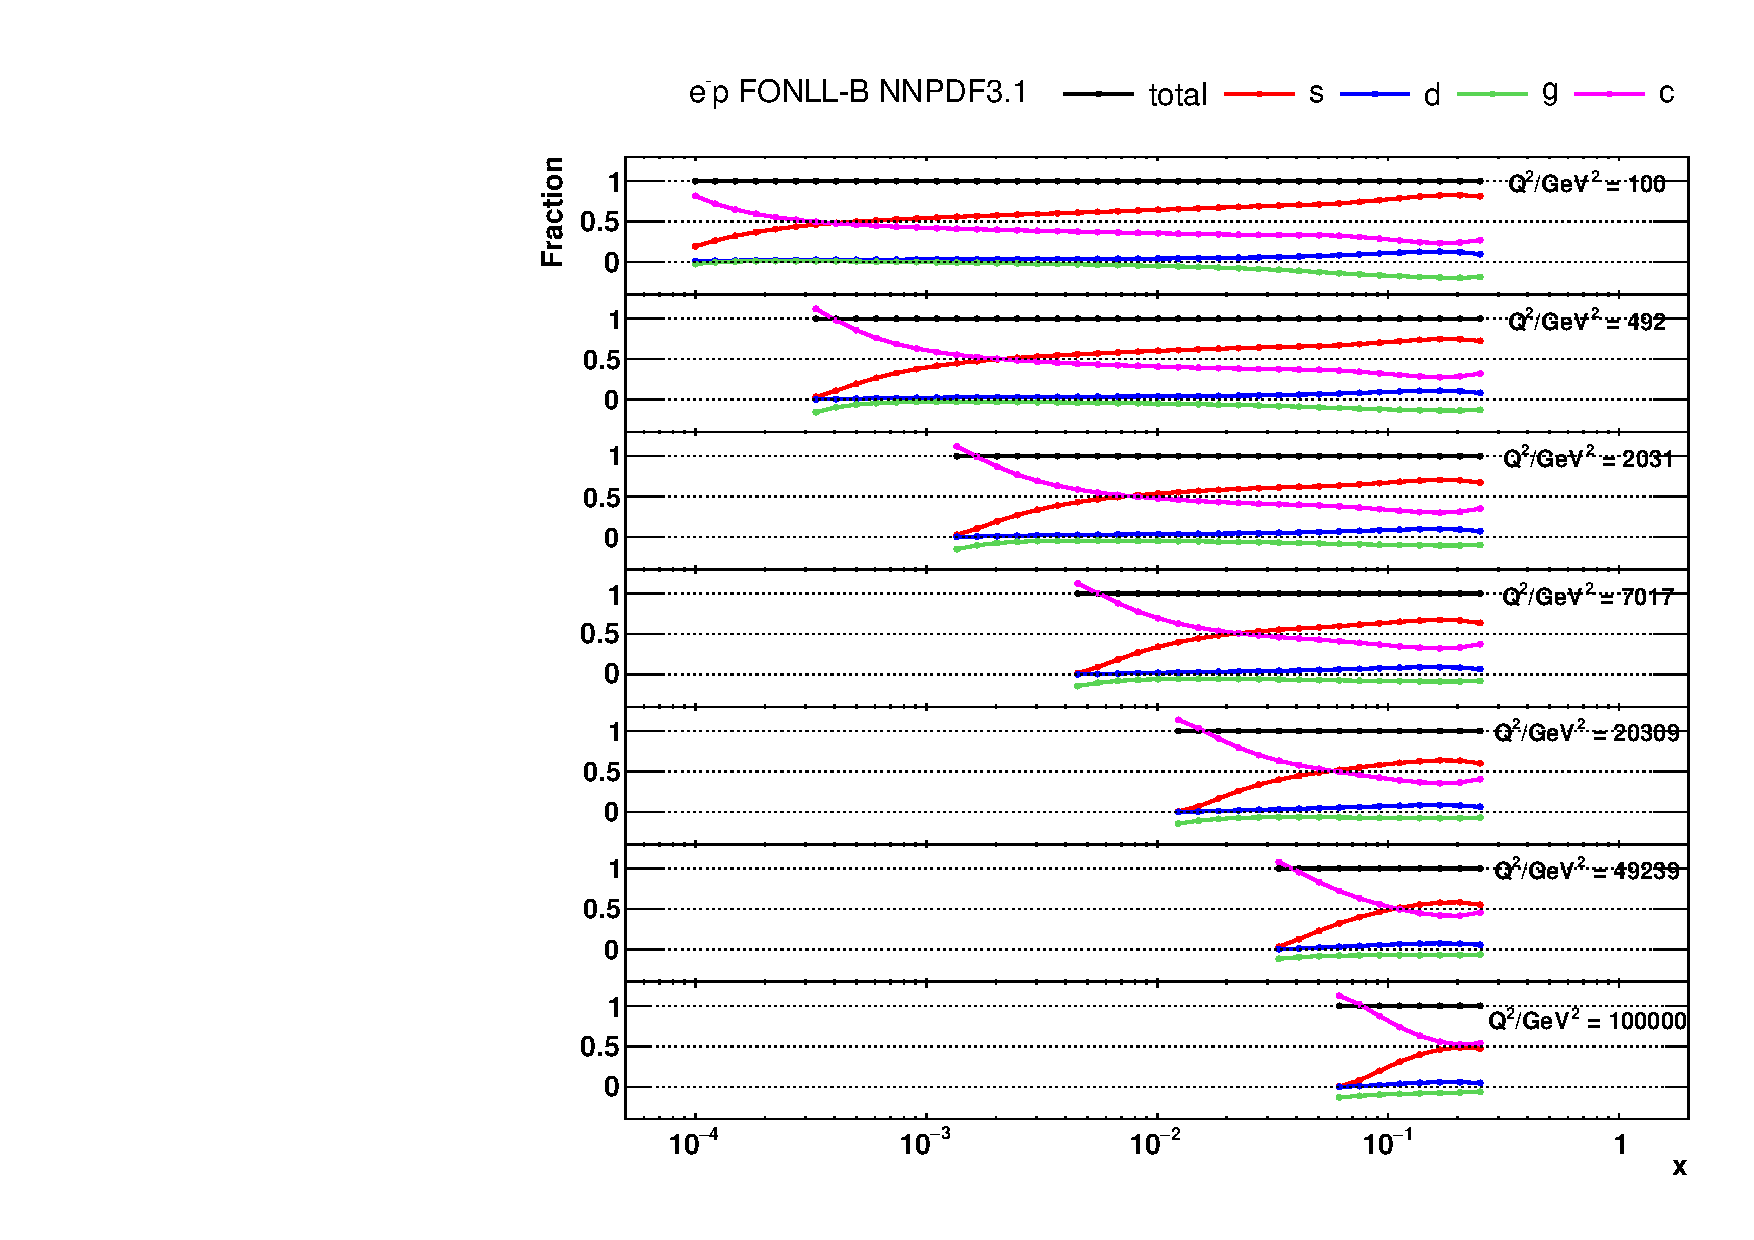
\includegraphics[width=0.49\textwidth]{pics/plots-110818/plot-parton-x-em-FONLL.pdf}}}
    \caption{The partonic subprocesses for charm CC production cross sections in the \ffns (left) and \fonll (right) schemes as a function of \xbj for different values of $Q^2$.}
    \label{fig:partonic-x}
\end{figure*}

\begin{figure*}
    \centering
    \centering{{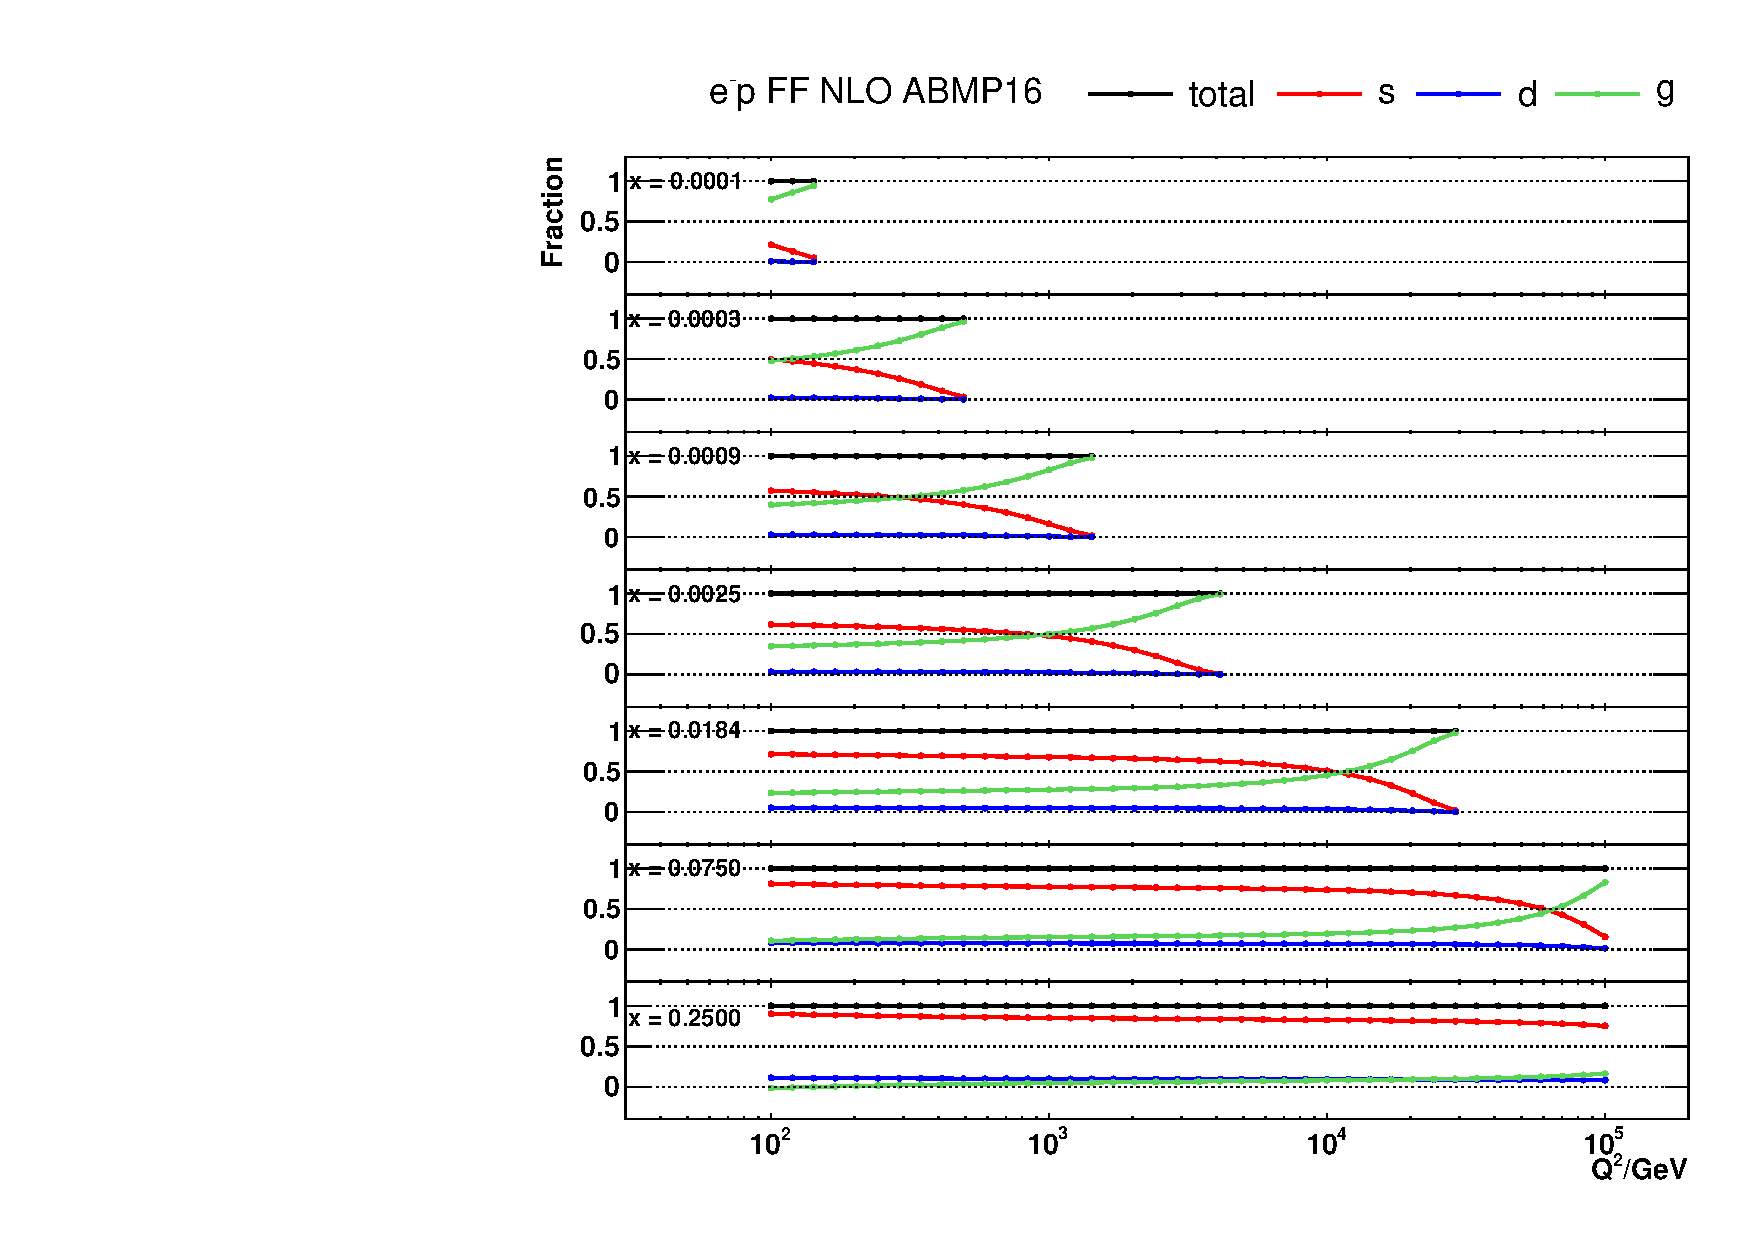
\includegraphics[width=0.49\textwidth]{pics/plots-110818/plot-parton-q2-em-FFABM.pdf}}}
    \centering{{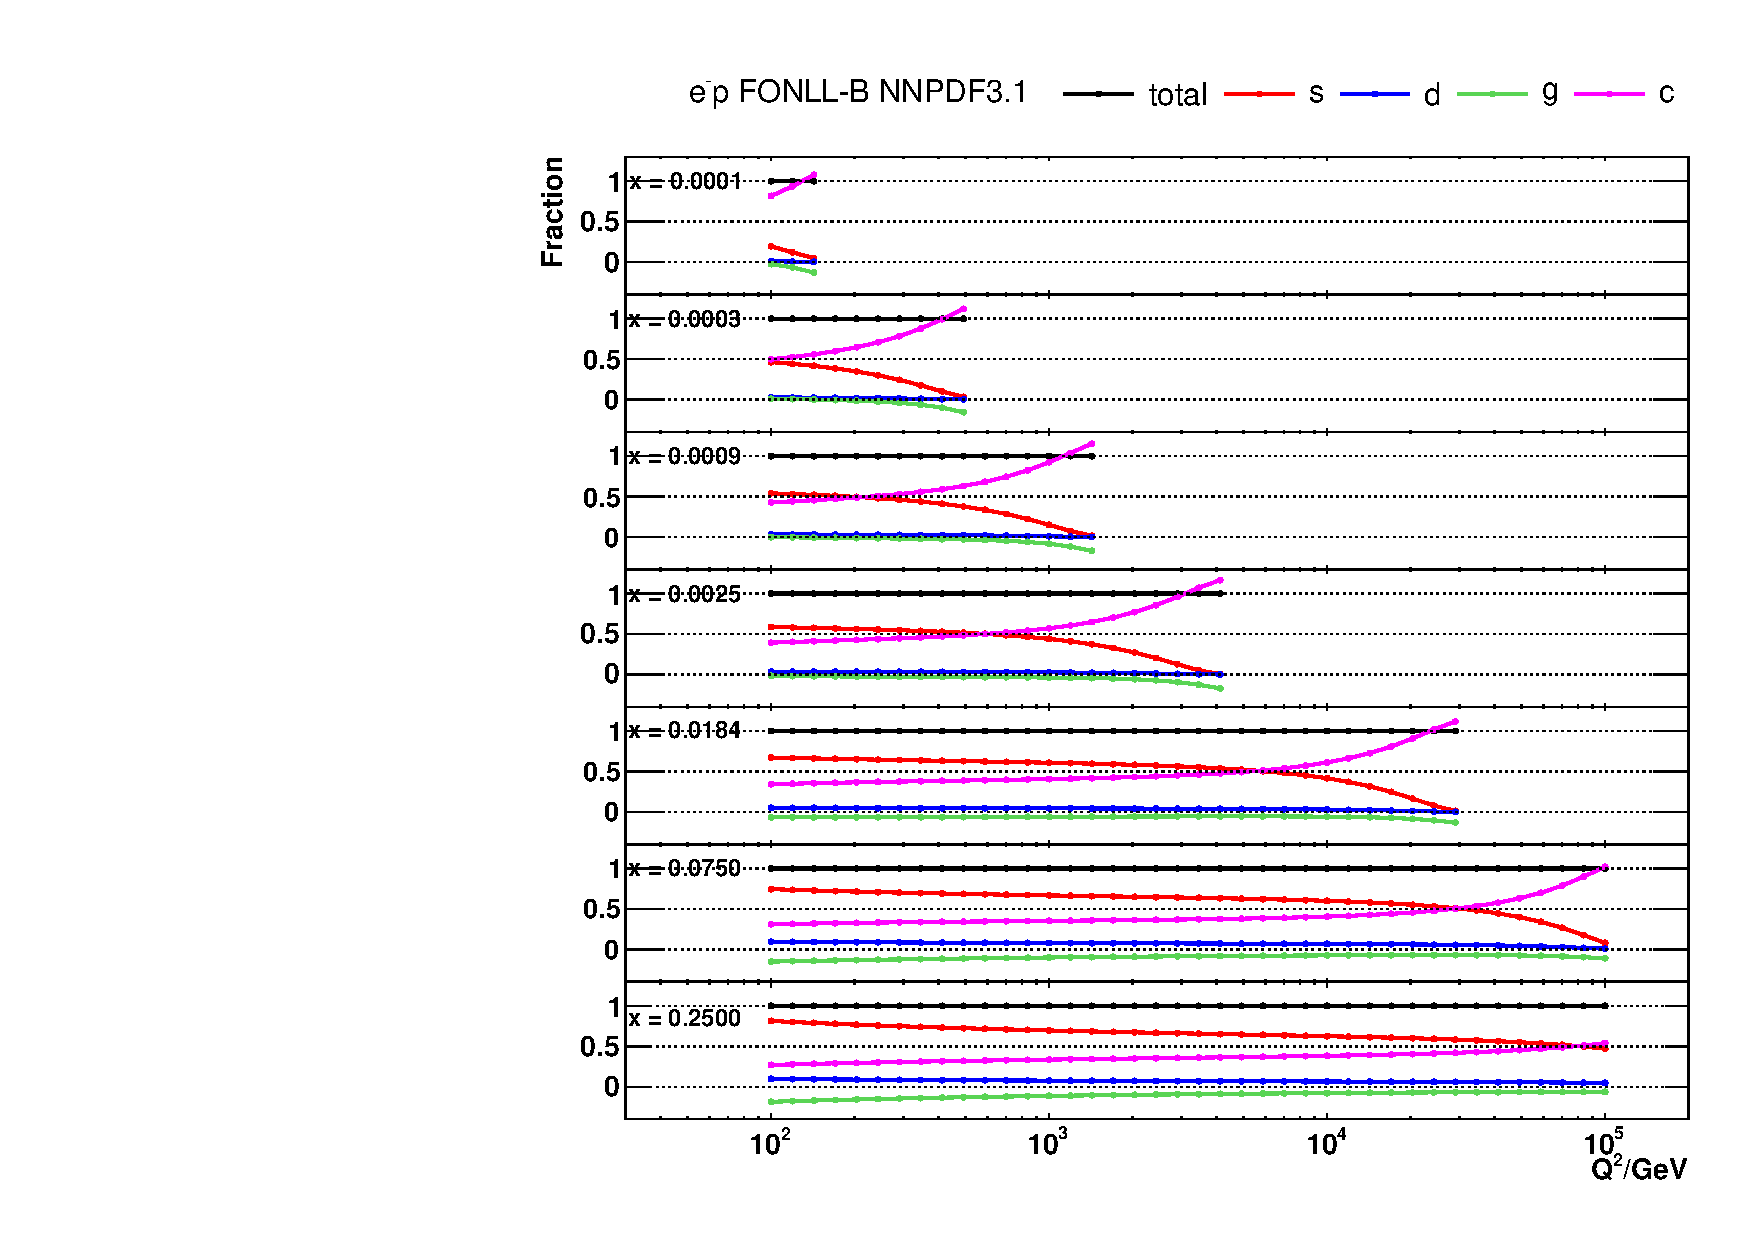
\includegraphics[width=0.49\textwidth]{pics/plots-110818/plot-parton-q2-em-FONLL.pdf}}}
    \caption{The partonic subprocesses for charm CC production cross sections in the \ffns (left) and \fonll (right) schemes as a function of $Q^2$ for different values of \xbj.}
    \label{fig:partonic-q2}
\end{figure*}

\begin{figure*}
    \centering
    \centering{{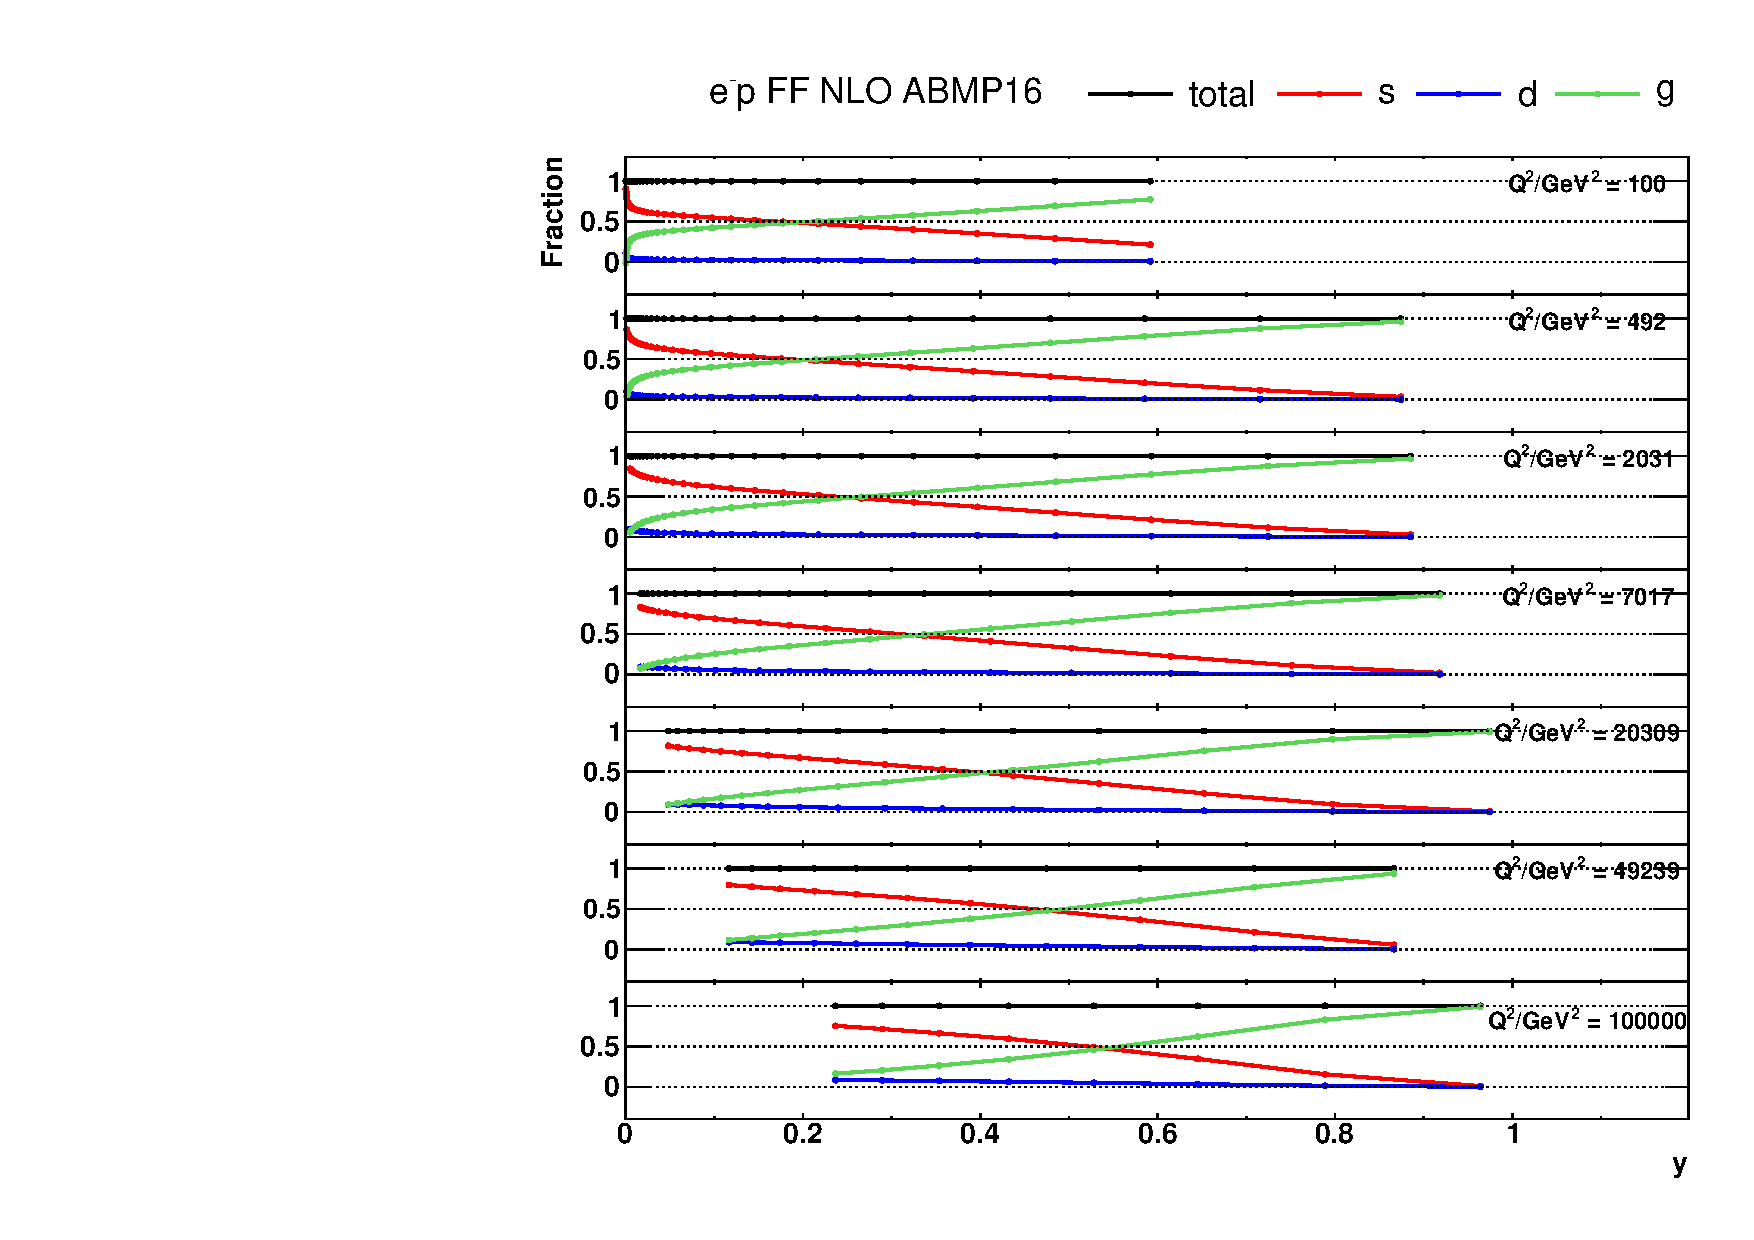
\includegraphics[width=0.49\textwidth]{pics/plots-110818/plot-parton-y-em-FFABM.pdf}}}
    \centering{{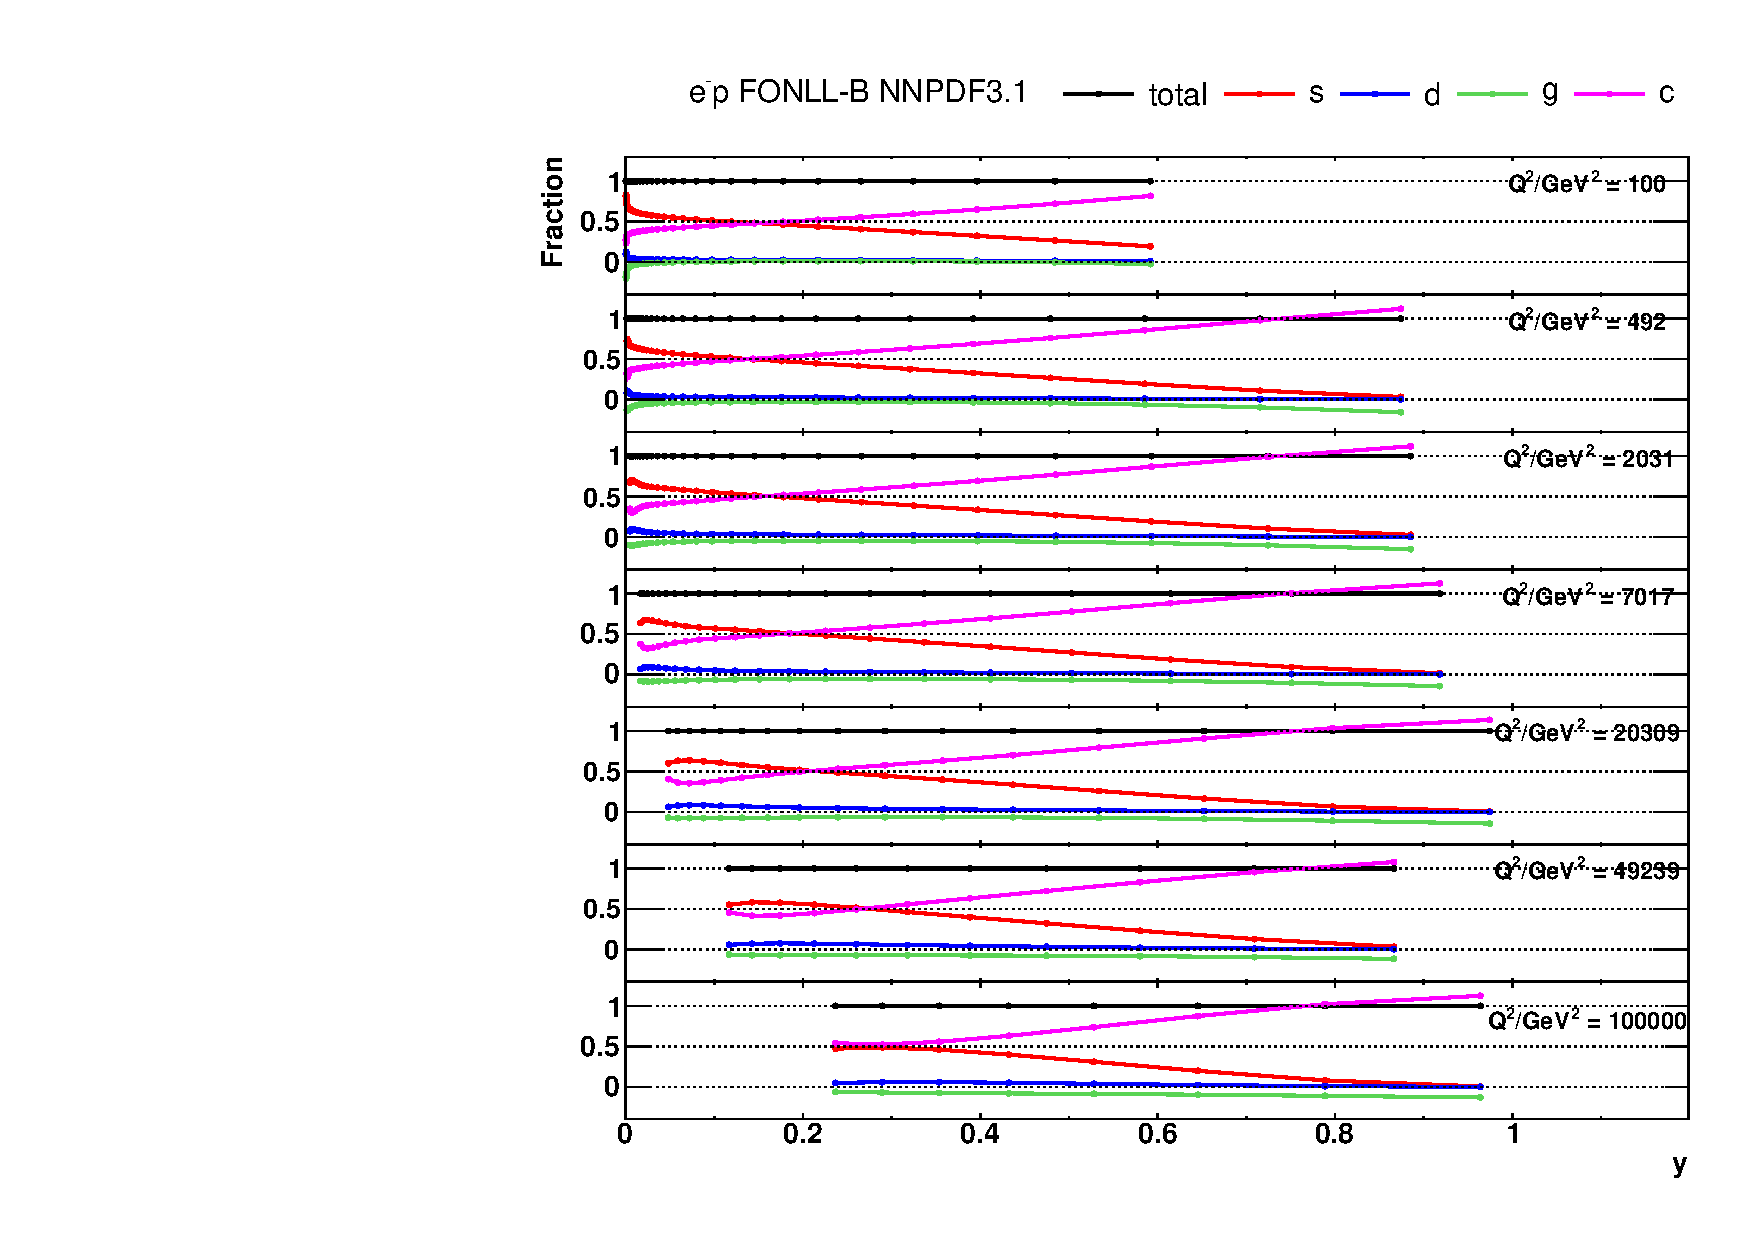
\includegraphics[width=0.49\textwidth]{pics/plots-110818/plot-parton-y-em-FONLL.pdf}}}
    \caption{The partonic subprocesses for charm CC production cross sections in the \ffns (left) and \fonll (right) schemes as a function of $y$ for different values of $Q^2$.}
    \label{fig:partonic-y}
\end{figure*}


\color{blue} %%%%%%%%%%%%%%%%%%%%%%%%%%%%%%%%%%%

Figures 7,8,9*** display a particularly interesting pattern; 
the gluon contribution for the FFNS  is strikingly similar to the charm contribution 
in the VFNS. 

In the FFNS, the charm is produced  predominantly from the explicit process $g \gamma\to c\bar{c}$. 
In contrast, for the VFNS the  $g\to c\bar{c}$ splitting is implicit (internal to the proton and evolved 
with the DGLAP evolution equations); the charm parton then emerges from the proton
to participate in the $c \gamma \to c$ process. 
%
The fundamental underlying process is the same in both the FFNS and VFNS, but 
the factorization boundary between the PDF and the hard scattering cross section, 
$f \otimes \hat{\sigma}$,  
(determined by $\mu$ and the scheme choice) is 
different.\footnote{Note 
there is a ``subtraction'' term  ($g\to c\bar{c} \otimes c \gamma \to c$) which closely 
matches the LO $c \gamma \to c$ process, but this ${\cal O}(\alpha \, \alpha_S)$  process is contained in the NLO gluon-initiated contribution.}



\color{black} %%%%%%%%%%%%%%%%%%%%%%%%%%%%%%%%%%%



\section{PDF constraints from charm CC pseudodata}
\label{sec:PDF}

The impact of charm CC cross section measurements at the LHeC on the PDFs is quantitatively estimated using a profiling technique~\cite{Paukkunen:2014zia}. This technique is based on minimizing \chisq between data and theoretical predictions taken into account both experimental and theoretical uncertainties arising from PDF variations. Two NLO PDF sets were chosen for this study: 
\abmp~\cite{Alekhin:2018pai} and \nnpdf~\cite{Ball:2017nwa} available via the \lhapdf interface (version 6.1.5)~\cite{Buckley:2014ana}. 
All PDF sets are provided with uncertainties in the format of eigenvectors. 

For this study, pseudodata representing measurements of charm CC production cross sections as a function of $Q^2$ and $x$ are used. {\bf [TODO: describe how pseudodata were produced]}
The study is performed using the \xfitter program (version 2.0.0)~\cite{Alekhin:2014irh}, an open-source QCD fit framework for PDF determination. The theoretical predictions are calculated at NLO QCD in the FFNS with the number of active flavours $n_f = 3$ and FONLL-B with $n_f = 5$. The running charm mass is set to $m_c(m_c) = 1.27$ GeV and $\alpha_s$ is set to the value used for the corresponding PDF extraction.
The renormalisation and factorisation scales are chosen to be $\mu_\mathrm{r} = \mu_\mathrm{f} = Q^2$.

The \chisq value is calculated as follows:
\begin{equation}
\chisq = \mathbf{R}^{T}_{} \mathbf{Cov}^{-1}_{} \mathbf{R}_{} + \sum_{\beta} b_{\beta,\rm th}^2,~~~\mathbf{R} = \mathbf{D} - \mathbf{T} - \sum_{\beta} \Gamma^{}_{\beta,\rm th} b_{\beta,\rm th},
\label{eq:chisq}
\end{equation}

where $\mathbf{D}$ and $\mathbf{T}$ are the column vectors of the measured and predicted values, respectively, 
and the correlated theoretical PDF uncertainties are included using the nuisance parameter vector $\boldsymbol{b_{\rm th}}$ with their influence on the theory predictions described by $\Gamma^{}_{\beta,\rm th}$, where index $\beta$ runs over all PDF eigenvectors. 
For each nuisance parameter a penalty term is added to the \chisq, representing the prior knowledge of the parameter. 
No theoretical uncertainties except the PDF uncertainties are considered.
The full covariance matrix representing the statistical and systematic uncertainties of the data is used in the fit. The statistical and systematic uncertainties are treated as additive, i.e., they do not change in the fit. The systematic uncertainties are assumed uncorrelated between bins.

To treat the asymmetric PDF uncertainties of the \nnpdf set, the \chisq function in Eq.~\ref{eq:chisq} is generalised assuming a parabolic dependence of the prediction on the nuisance parameter~\cite{Alekhin:2014irh}:
\begin{eqnarray}
\Gamma^{}_{\beta, \rm th} \to \Gamma^{}_{\beta, \rm th} +  \Omega^{}_{\beta, \rm th}b_{\beta, \rm th}\,, \label{eq:iter}
\end{eqnarray}
where $\Gamma^{}_{\beta, \rm th} = 0.5(\Gamma^{+}_{\beta, \rm th} - \Gamma^{-}_{\beta, \rm th})$ and $\Omega^{}_{\beta} = 0.5(\Gamma^{+}_{\beta, \rm th}
+ \Gamma^{-}_{\beta, \rm th})$ are determined from the shifts of predictions corresponding to up ($\Gamma^{+}_{\beta, \rm th}$) and down ($ \Gamma^{-}_{\beta, \rm th}$) PDF uncertainty eigenvectors.

The values of the nuisance parameters at the minimum, $b^{\rm min}_{\beta,\rm th}$ are interpreted as optimised, or profiled, PDFs, while their uncertainties determined using the tolerance criterion of $\Delta\chi^2 = 1$ correspond to the new PDF uncertainties. The profiling approach assumes that the new data are compatible with theoretical predictions using the existing PDFs, such that no modification of the PDF fitting procedure is needed. Under this assumption, the central values of the measured cross sections are set to the central values of the theoretical predictions. 

The original and profiled \abmp and \nnpdf PDF uncertainties are shown in Figs.~\ref{fig:pdf-abmp}--\ref{fig:pdf-nnpdf-100000}. 
The uncertainties of the PDFs are presented at the scales $\mu_\mathrm{f}^2=100$ GeV$^2$ and $\mu_\mathrm{f}^2=100000$ GeV$^2$.
A strong impact of the charm CC pseudodata on the PDFs is observed for both PDF sets.
In particular, the uncertainties of the strange PDF are strongly reduced once the pseudodata are included in the fit. 
Also the gluon PDF uncertainties are decreased. Furthermore, in the case of the NNPDF3.1 set and FONLL scheme, the charm PDF uncertainties are reduced significantly.

\begin{figure}
    \centering
    {{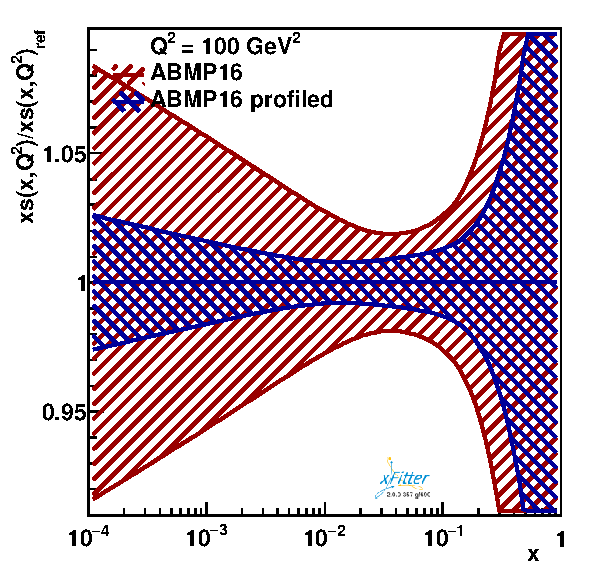
\includegraphics[width=0.235\textwidth]{pics/pdf-profile-ffabm/q2_100_pdf_s_ratio.pdf}}}
    {{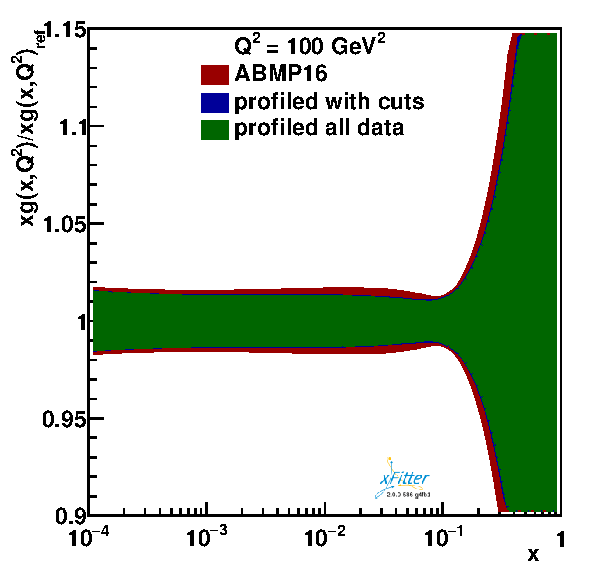
\includegraphics[width=0.235\textwidth]{pics/pdf-profile-ffabm/q2_100_pdf_g_ratio.pdf}}}\\
    {{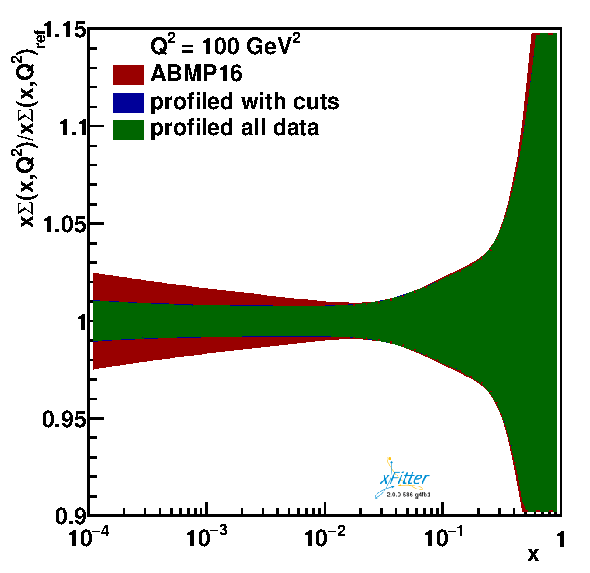
\includegraphics[width=0.235\textwidth]{pics/pdf-profile-ffabm/q2_100_pdf_Sea_ratio.pdf}}}
    {{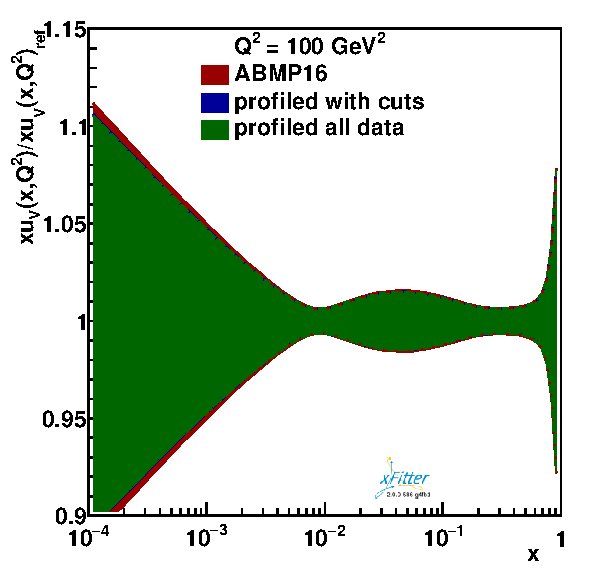
\includegraphics[width=0.235\textwidth]{pics/pdf-profile-ffabm/q2_100_pdf_uv_ratio.pdf}}}
    {{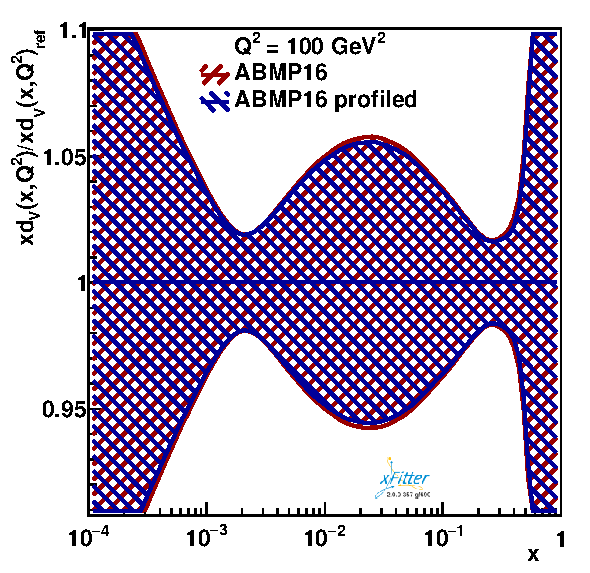
\includegraphics[width=0.235\textwidth]{pics/pdf-profile-ffabm/q2_100_pdf_dv_ratio.pdf}}}
    \caption{The relative strange (top left), gluon (top right), sea quark (middle left), u valence quark (middle right) and d valence quark (bottom) PDF uncertainties at $\mu_\mathrm{f}^2=100$ GeV$^2$ of the original and profiled \abmp PDF set.}
    \label{fig:pdf-abmp}
\end{figure}

\begin{figure}
    \centering
    {{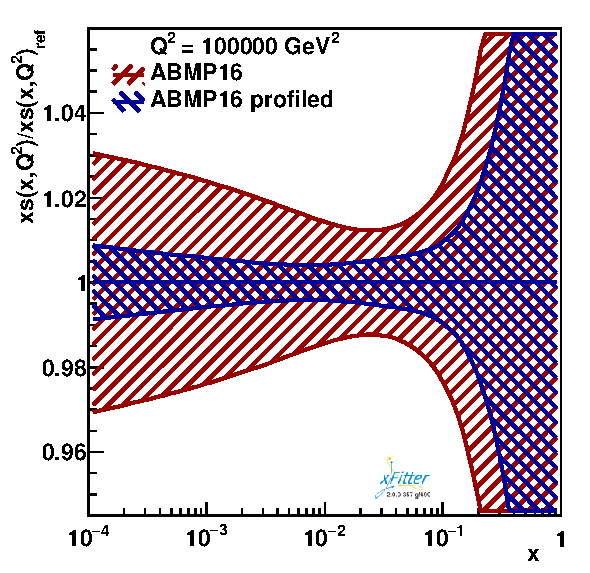
\includegraphics[width=0.235\textwidth]{pics/pdf-profile-ffabm/q2_100000_pdf_s_ratio.pdf}}}
    {{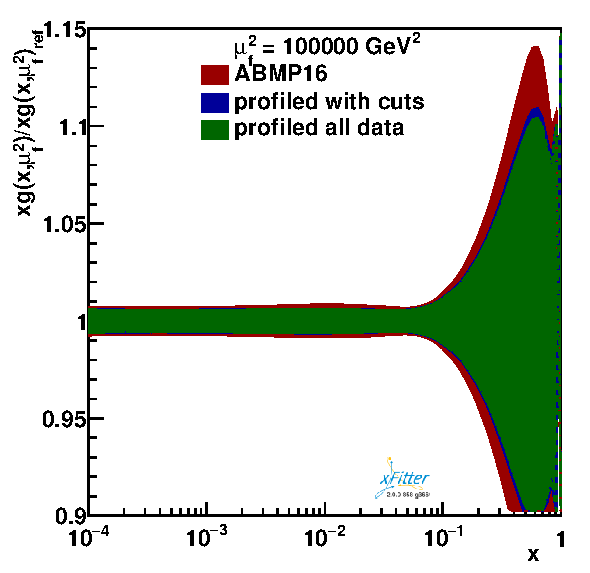
\includegraphics[width=0.235\textwidth]{pics/pdf-profile-ffabm/q2_100000_pdf_g_ratio.pdf}}}\\
    {{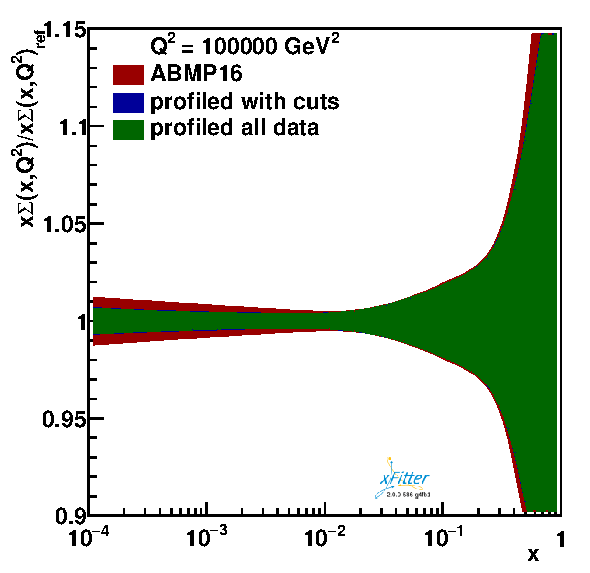
\includegraphics[width=0.235\textwidth]{pics/pdf-profile-ffabm/q2_100000_pdf_Sea_ratio.pdf}}}
    {{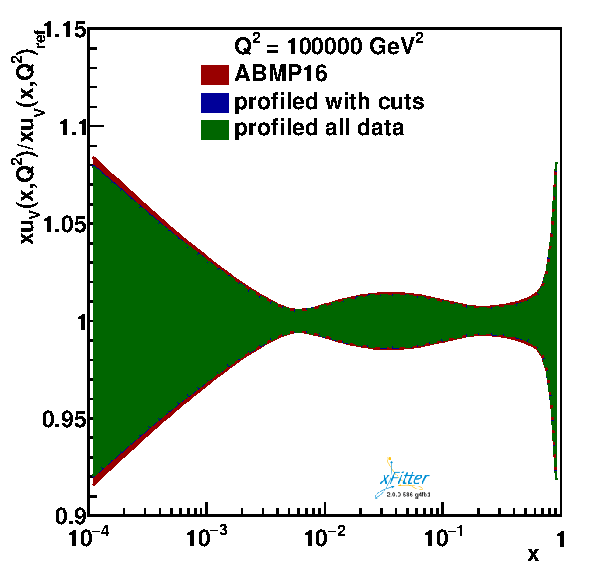
\includegraphics[width=0.235\textwidth]{pics/pdf-profile-ffabm/q2_100000_pdf_uv_ratio.pdf}}}
    {{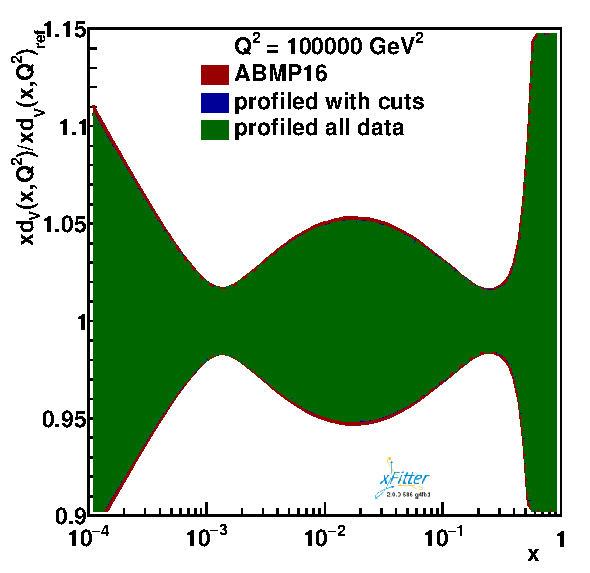
\includegraphics[width=0.235\textwidth]{pics/pdf-profile-ffabm/q2_100000_pdf_dv_ratio.pdf}}}
    \caption{The relative strange (top left), gluon (top right), sea quark (middle left), u valence quark (middle right) and d valence quark (bottom) PDF uncertainties at $\mu_\mathrm{f}^2=100000$ GeV$^2$ of the original and profiled \abmp PDF set.}
    \label{fig:pdf-abmp-100000}
\end{figure}

\begin{figure}
    \centering
    {{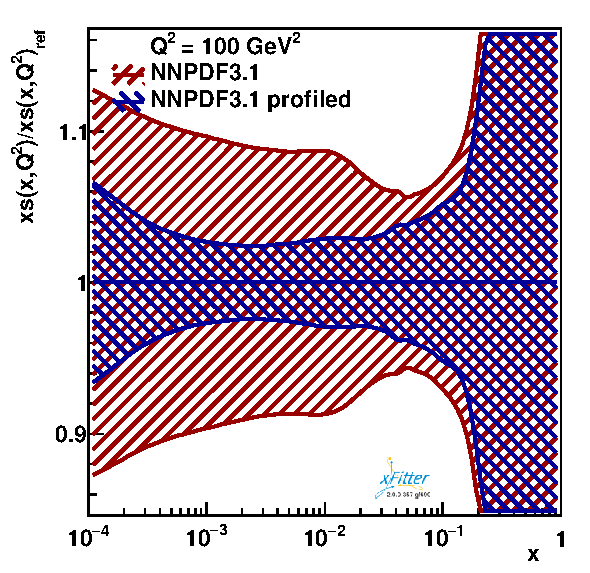
\includegraphics[width=0.235\textwidth]{pics/pdf-profile-fonll/q2_100_pdf_s_ratio.pdf}}}
    {{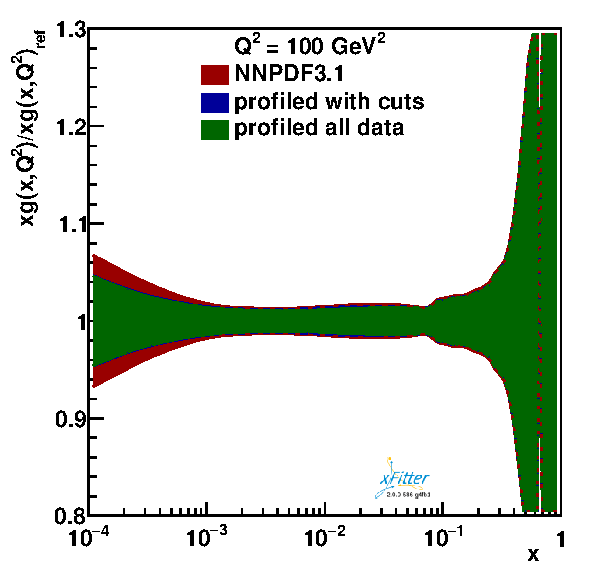
\includegraphics[width=0.235\textwidth]{pics/pdf-profile-fonll/q2_100_pdf_g_ratio.pdf}}}\\
    {{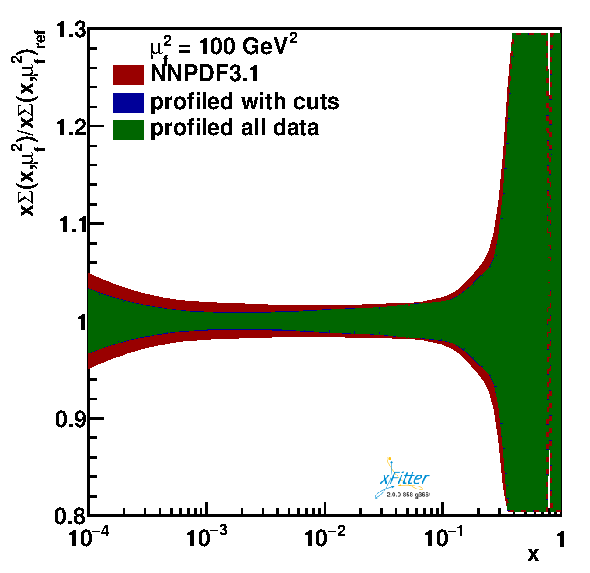
\includegraphics[width=0.235\textwidth]{pics/pdf-profile-fonll/q2_100_pdf_Sea_ratio.pdf}}}
    {{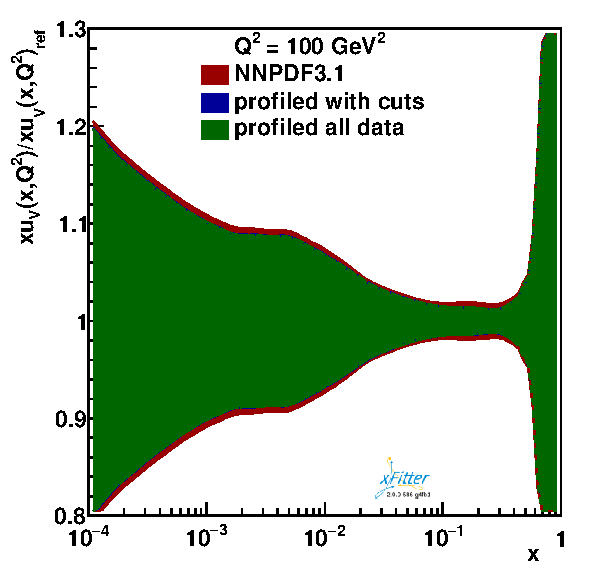
\includegraphics[width=0.235\textwidth]{pics/pdf-profile-fonll/q2_100_pdf_uv_ratio.pdf}}}
    {{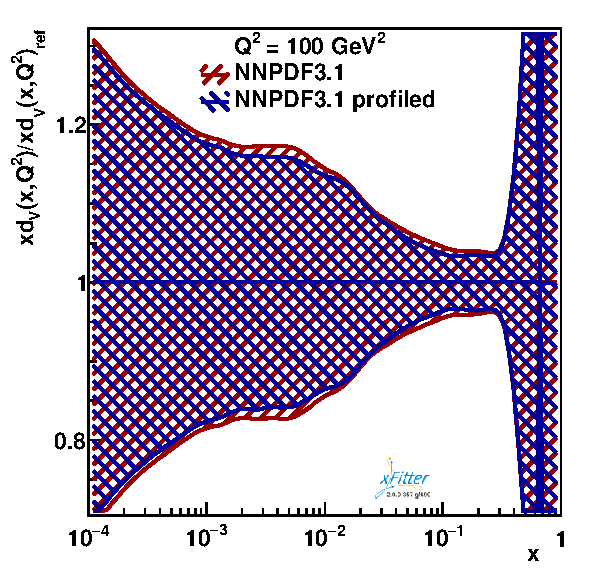
\includegraphics[width=0.235\textwidth]{pics/pdf-profile-fonll/q2_100_pdf_dv_ratio.pdf}}}
    {{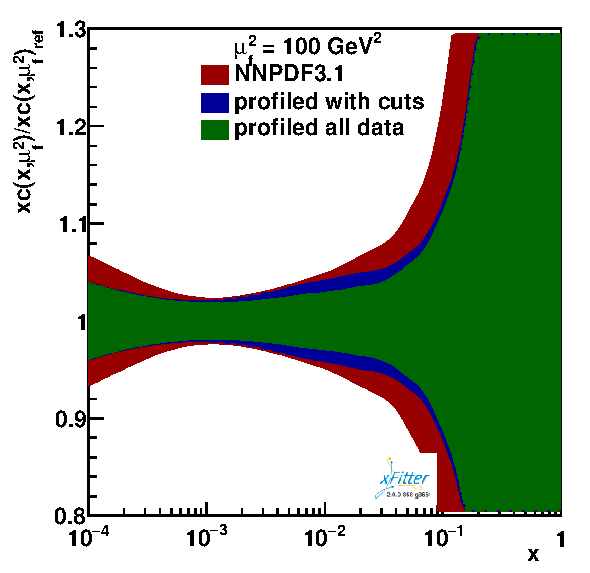
\includegraphics[width=0.235\textwidth]{pics/pdf-profile-fonll/q2_100_pdf_c_ratio.pdf}}}
    \caption{The relative strange (top left), gluon (top right), sea quark (middle left), u valence quark (middle right), d valence quark (bottom left) and charm quark (bottom right) PDF uncertainties at $\mu_\mathrm{f}^2=100$ GeV$^2$ of the original and profiled \nnpdf PDF set.}
    \label{fig:pdf-nnpdf}
\end{figure}

\begin{figure}
    \centering
    {{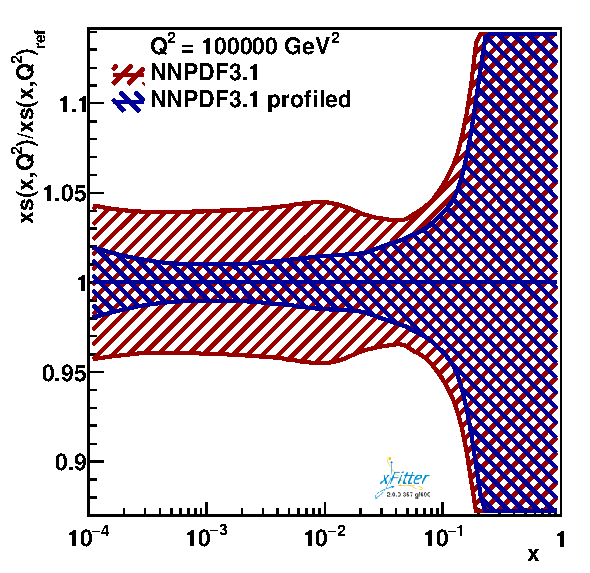
\includegraphics[width=0.235\textwidth]{pics/pdf-profile-fonll/q2_100000_pdf_s_ratio.pdf}}}
    {{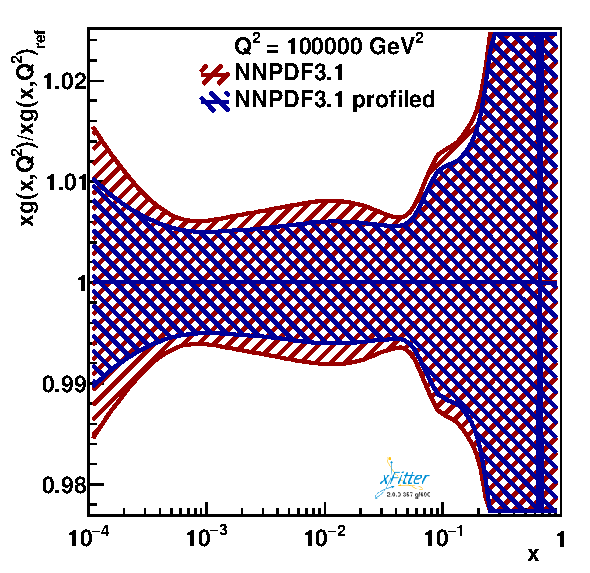
\includegraphics[width=0.235\textwidth]{pics/pdf-profile-fonll/q2_100000_pdf_g_ratio.pdf}}}\\
    {{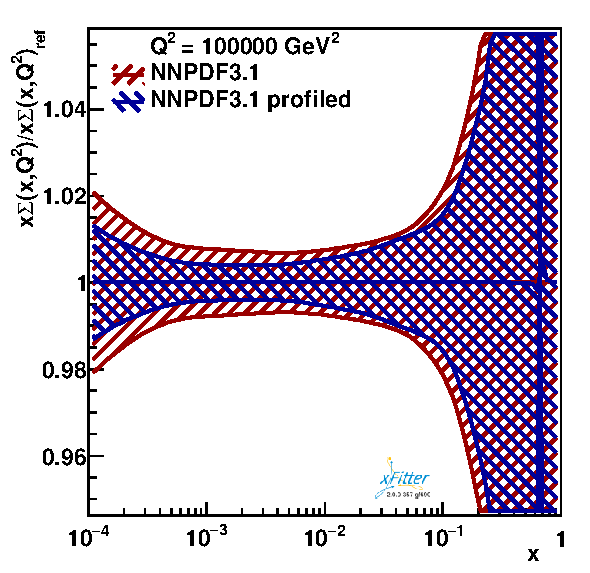
\includegraphics[width=0.235\textwidth]{pics/pdf-profile-fonll/q2_100000_pdf_Sea_ratio.pdf}}}
    {{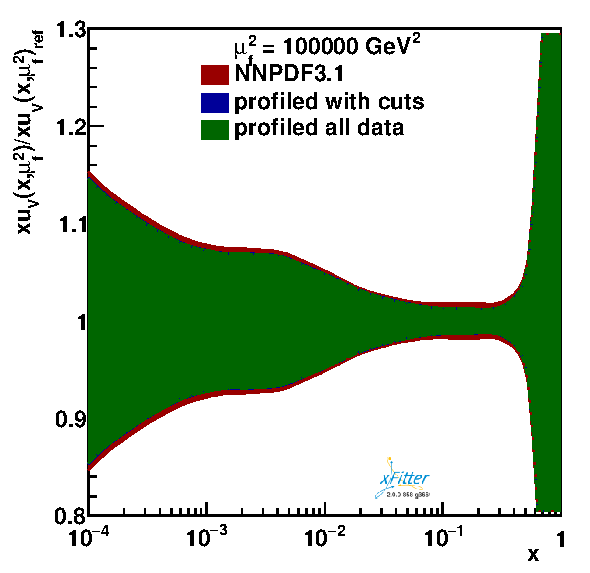
\includegraphics[width=0.235\textwidth]{pics/pdf-profile-fonll/q2_100000_pdf_uv_ratio.pdf}}}
    {{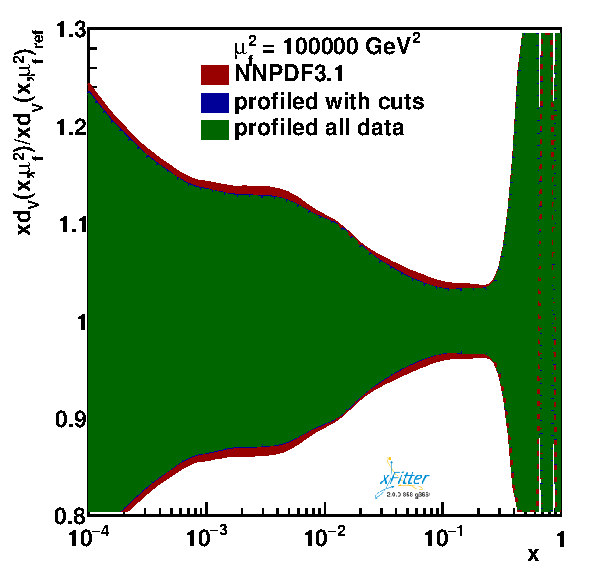
\includegraphics[width=0.235\textwidth]{pics/pdf-profile-fonll/q2_100000_pdf_dv_ratio.pdf}}}
    {{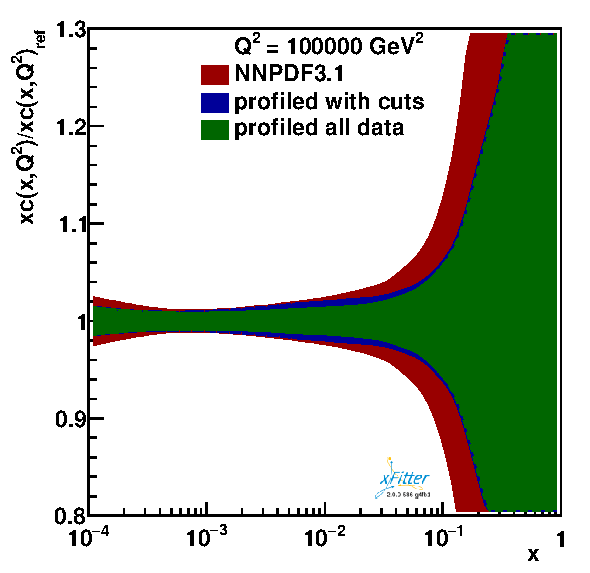
\includegraphics[width=0.235\textwidth]{pics/pdf-profile-fonll/q2_100000_pdf_c_ratio.pdf}}}
    \caption{The relative strange (top left), gluon (top right), sea quark (middle left), u valence quark (middle right), d valence quark (bottom left) and charm quark (bottom right) PDF uncertainties at $\mu_\mathrm{f}^2=100000$ GeV$^2$ of the original and profiled \nnpdf PDF set.}
    \label{fig:pdf-nnpdf-100000}
\end{figure}

\section{Discussion and summary}

\begin{acknowledgements}
%  We would like to thank Juan Rojo for a cri\-ti\-cal reading of this
%  paper, and Luca Rottoli for discussions on the description of charm
%  data.  V.~B.\ and F.~G.\ are supported by the European Research
%  Council Starting Grant ``PDF4BSM''.  Additional support was received
%  by A.~G., A.~S.\ and P.~S.\ from the BMBF-JINR cooperation program
%  and the Heisenberg-Landau program.  A.~L.\ is supported by the
%  Polish Ministry under program Mobility Plus, no 1320/MOB/IV/2015/0.
%  M.~B.\ is supported by the by the Marie Sk\l{}odowska Curie grant
%  HiPPiE@LHC.
\end{acknowledgements}


%%%%%%%%%%%%%%%%%%%%%%%%%%%%%%%%%%%%%%%%%
%  %% LyX 2.3.1 created this file.  For more info, see http://www.lyx.org/.
%  %% Do not edit unless you really know what you are doing.
%  \documentclass[twocolumn,english,showpacs,preprintnumbers,amsmath,amssymb,floatfix]{revtex4-1}
%  \usepackage[T1]{fontenc}
%  \usepackage[latin9]{inputenc}
%  \setcounter{secnumdepth}{3}
%  \usepackage{color}
%  \usepackage{babel}
%  \usepackage{graphicx}
%  \usepackage{esint}
%  \usepackage[unicode=true,
%   bookmarks=false,
%   breaklinks=false,pdfborder={0 0 1},backref=section,colorlinks=false]
%   {hyperref}
%  
%  \makeatletter
%  %%%%%%%%%%%%%%%%%%%%%%%%%%%%%% User specified LaTeX commands.
%  \hyphenpenalty=10000
%  
%  \makeatother
%  
%  \begin{document}
%  
\clearpage
\newcommand{\xsec}[1]{\vskip 6pt \noindent {\bf #1} \quad }

\appendix

{\small
\textbf{\textcolor{blue}{TO DO LIST:}}
\textcolor{blue}{{*} Follow up on John Collins' list {[}MOSTLY DONE{]} }
\textcolor{blue}{{*} Add brief mention at end that this applies also
to bottom quark {[}at end{]}}
\textcolor{blue}{{*} refs from Sasha: LHC W+c measurements:
  \cite{Chatrchyan:2013uja,Aad:2014xca,Sirunyan:2018hde}}
  }

\section{$F_{2}^{charm}$ Beyond Leading-Order}

\begin{figure}
\centering 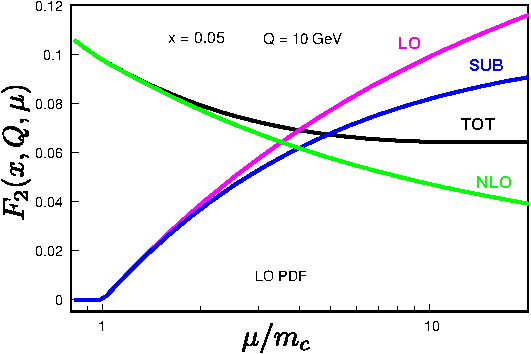
\includegraphics[clip,width=0.45\textwidth]{pics/fred/acot_fig}
\caption{Calculation of $F_{2}^{c}$ vs.\ $\mu$ in the VFNS illustrating the
cancellation of the LO ($\bar{c}W^{+}\to\bar{s}$) and the SUB \hbox{$(g\to \bar{c})$}$\otimes$\hbox{$(\bar{c}W^+ \to \bar{s})$}
contributions in the region $\mu\sim m_{c}$. The $Q$ scale is fixed
at $10\,$GeV and the charm PDF is matched at $\mu_{c}=m_{c}$ such
that $f_{c}(x,\mu=m_{c})=0$. \label{fig:acot}}
\end{figure}

\begin{figure*}
\centering 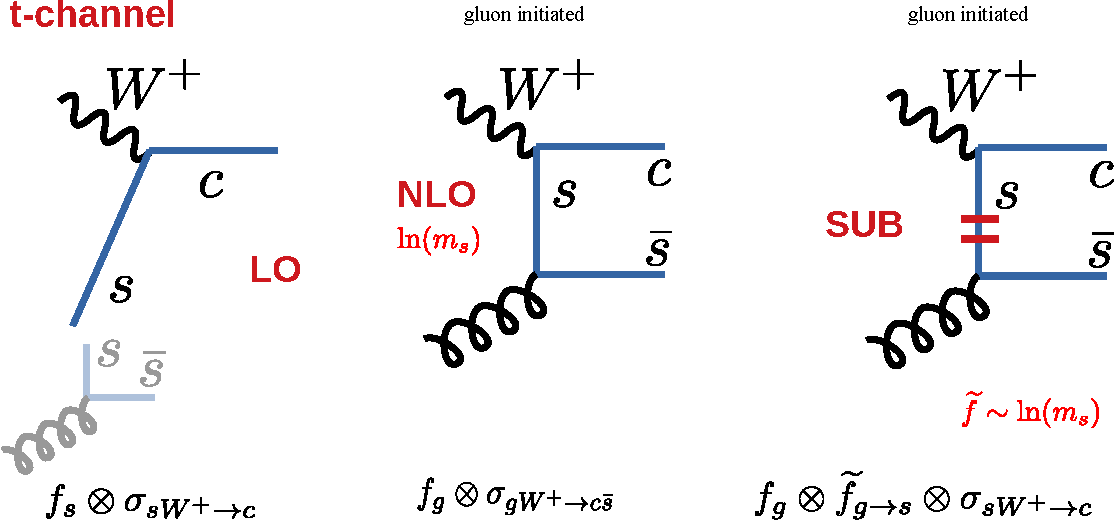
\includegraphics[clip,width=0.8\textwidth]{pics/fred/tchannel}
\caption{Gluon $t$-channel processes up to ${\cal  O}(\alpha_S^1)$.  \label{fig:tchannel}}
\end{figure*}

\begin{figure*}
\centering 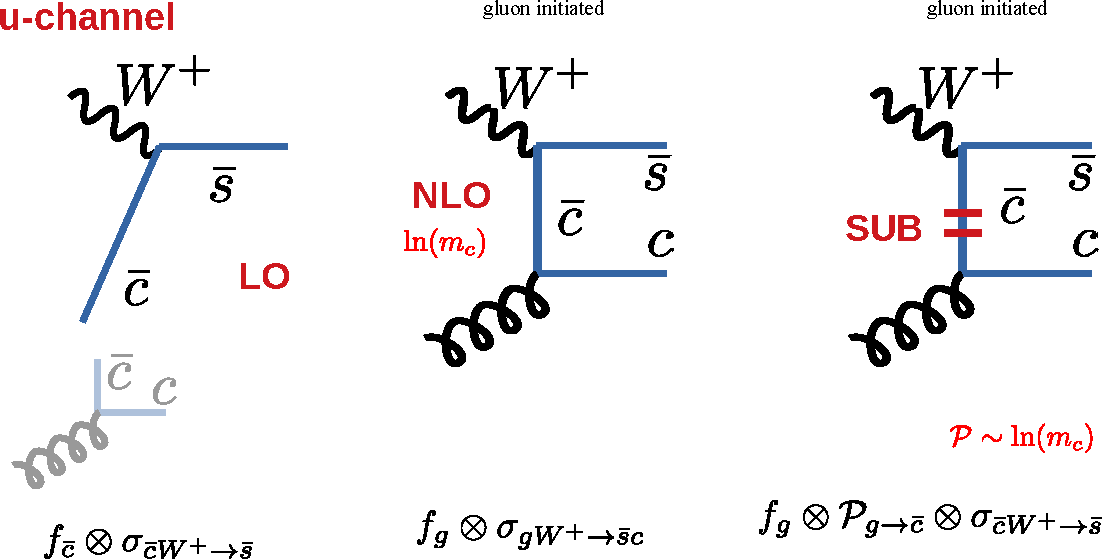
\includegraphics[clip,width=0.8\textwidth]{pics/fred/uchannel}
\caption{Gluon NLO $u$-channel processes  up to ${\cal  O}(\alpha_S^1)$. \label{fig:uchannel}}
\end{figure*}




\xsec{The Multi-Scale Problem:}
%
The charged current DIS charm production process involves some interesting
issues that we will explore here in detail. In particular, there are
multiple mass and energy scales which span a wide kinematic range,
and it becomes an intricate puzzle to treat them all properly. 

For this current illustration, we will focus on the contribution to
the DIS $F_{2}^{c}$ structure function from the process involving
the strange and charm quark; other quark combinations can be addressed
in a similar manner. In particular, we will show that as we go to
higher-orders the $F_{2}^{c}$ structure function must be defined
carefully so that i) theoretically it is free of divergences and independent
of the renormalization scales, and ii) experimentally it matches what
is measured by the detector.

\xsec{Overview:}
%

\textcolor{blue}{... to be filled in ... (what other detailed are needed???)}

\xsec{The Mass Scales:}
%
There are four mass scales that enter this process: $\{Q,\mu,m_{s},m_{c}\}$;
additionally, in the case of the VFNS we have the matching scale,
$\mu_{c}$.

The $Q$ scale is the invariant mass of the virtual boson probe ($W^{+}$
in this case), and can be related to the energy and angle of lepton;
this is a physically measurable kinematic variable. 

In contrast, the renormalization scale $\mu$ is an unphysical scale
used to factorize the PDF and the hard scattering cross section; thus,
the physics should be insensitive to a variation of $\mu$. As our
calculations typically involve the dimensionless combination $\ln(\mu^{2}/Q^{2})$,
we generally choose $\mu\sim Q$ avoid large logarithms. 

The strange quark is a ``light'' active parton with an associated
PDF $s(x)$ and mass $m_{s}$. The strange quark mass is comparable
or less than other hadronic scales which are neglected; as such, it
serves only as a regulator and plays no physical role, and we can
take $m_{s}\to0$ if we choose. 

The charm quark is a ``heavy'' object; its associated mass $m_{c}$
does play a physical role and cannot be neglected. There may or may
not be a PDF associated with the charm. In a 3-flavor FFNS scheme,
there is no charm PDF. In a 4-flavor VFNS there is a charm PDF only
when the $\mu$ scale is above the scale where the charm PDF is activated;
we call this the matching scale, $\mu_{c}$. It is common\footnote{The choice of matching scale $\mu_{c}=m_{c}$ is common because at
NLO the $\overline{MS}$ matching conditions on the PDFs are proportional
to the DGLAP kernel times $\ln(\mu/m_{c})$, as explicit calculation
shows the constant term vanishes; thus we have the simple boundary
condition $f_{c}(x,\mu=m_{c})=0$. At NNLO, the constant term is non-zero
and this yields $f_{c}(x,\mu=m_{c})\not=0$. See \cite{Stavreva:2012bs}
and references therein.} to set $\mu_{c}=m_{c}$, but this is not required.\footnote{By displacing the matching scale to larger values $\mu_{c}\gg m_{c}$,
can have the advantage of avoiding delicate cancellations in the region
$\mu\sim m_{c}$; this flexibility was explored in Refs.~\cite{Bertone:2017ehk,Bertone:2018ids}
.} In this study we will fix the matching scale to this common choice:
$\mu_{c}=m_{c}$.



What makes this process complex is there is no fixed hierarchy for
the mass scales, and we will need to compute both in the low $Q$
region where $Q\lesssim m_{c}$ as well as the high $Q$ region $Q\gg m_{c}$. 



Because there are two different quark masses $\{m_{s},m_{c}\}$ involved
in the charged current DIS flavor-changing process,  we can examine
the mass singularities of the $t$-channel and $u$-channel separately.
This separation is particularly useful to understand how the individual
mass singularities are addressed, and how FFNS and VFNS organize the
contributions to the total structure function. 

\xsec{3-Flavor FFNS:}
%
To be specific, we will consider charged-current DIS production of
a charm quark. We first compute this in a 3-flavor (FFNS) scheme where
$\{u,d,s\}$ are light ``active'' partons in the proton, and charm
$\{c\}$ is considered an external ``heavy'' particle. This can
be implemented in the ACOT scheme\cite{Aivazis:1993pi} for example
by using a CWZ renormalization\cite{Collins:1978wz} where the light
``active'' partons are renormalized with normal $\overline{MS}$,
and the ``heavy'' quarks use a zero-momentum subtraction. In this
scheme, the \textbf{leading-order} (LO) process is \mbox{$sW^{+}\to c$}
as illustrated in Fig.\,\ref{fig:acot}. At \textbf{next-to-leading-order}
(NLO), we then include \mbox{$gW^{+}\to c\bar{s}$} which has both $t$-channel
and $u$-channel contributions.\footnote{Note, there are also corresponding quark-initiated processes; we will
focus on the gluon-initiated processes as this is sufficient to illustrate
our points. Both the gluon- and quark-initiated contributions are
included in our calculations. }

\xsec{$t$-Channel:}
%
The $t$-channel process has an intermediate $s$-quark exchanged, and
if we use the strange quark mass $m_{s}$ to regulate the singularities,
this will yield a contribution proportional to $\ln(Q/m_{s})$. This
mass singularity arises from the region of phase space where the exchanged
$s$-quark becomes collinear and close to the mass-shell; that is,
when the phase space of the \mbox{$gW^{+}\to c\bar{s}$} process begins to
overlap with that of the \mbox{$sW^{+}\to c$} process. This ``double counting''
is resolved by a \textbf{subtraction} (SUB) counter-term
%(which is formally part of the NLO contribution)
given by:
\[
(SUB)\sim f_{g}\otimes\widetilde{f}{}_{g\to s}\otimes\sigma_{sW^{+}\to c}\quad.
\]
Here, $\widetilde{f}{}_{g\to s}$ is the perturbative splitting of
the gluon into an $s\bar{s}$ pair; the leading term is proportional
to:\footnote{The scale of the SUB term is $\mu$ as the relevant scale here is
the renormalization scale of the PDF:$f(x,\mu)\otimes\hat{\sigma}(x,Q,\mu)$. }
\[
\widetilde{f}_{g\to s}(x,\mu)\sim\frac{\alpha_{S}(\mu)}{2\pi}P_{g\to s}^{(1)}(x)\:\ln\left(\frac{\mu^{2}}{m_{s}^{2}}\right)+\text{{\cal O}}(\alpha_{s}^{2})
\]
 where $P_{g\to s}^{(1)}(x)$ is the $\alpha_{S}^{1}$ DGLAP splitting
kernel for \hbox{$g\to s$}.

The complete contribution to the structure function is given by:
\[
F_{2}^{c}\sim TOT=LO+(NLO-SUB)
\]
The complete ${\cal O}(\alpha_{s}^{1})$ contribution is the combination
$(NLO-SUB)$; our separation into $NLO$ and $SUB$ is simply to illustrate
the interplay of these components. Both the NLO and SUB terms have
$\ln(m_{s})$ divergences, but these precisely cancel and yield a
well defined result even as we take the $m_{s}\to0$ limit.\footnote{In fact, we could have taken $m_{s}=0$ initially and used dimensional
regularization to compute the contributions.}

\xsec{$u$-Channel:}
%
We next examine the $u$-channel NLO contribution to the \mbox{$gW^{+}\to c\bar{s}$}
process. This has an intermediate $c$-quark exchanged, and is proportional
to $\ln(Q/m_{c})$. In the FFNS where the charm is a ``heavy'' non-parton,
there is no counter-term for this graph, and the resulting observables
will retain the $\ln(Q/m_{c})$ dependence. In principle, this means
when we go to large $Q$-scales, these terms will begin to degrade
the convergence of our perturbation series. In practice, while this
degradation only grows logarithmically, at large scales (such as at
the LHC) we do find it convenient to treat the charm on an equal-footing
as the ${u,d,s}$ partons. 

\xsec{4-Flavor VFNS:}
%
We now turn to the 4-flavor (VFNS) scheme where we include the charm
quark as an ``active'' parton and compute its associated PDF.

In this case, there is a $u$-channel counter-term (SUB) given by $f_{g}\otimes\widetilde{f}{}_{g\to\bar{c}}\otimes\sigma_{\bar{c}W^{+}\to\bar{s}}$
which is proportional to $\ln(\mu/m_{c})$. The NLO $u$-channel contribution
will have a $\ln(Q/m_{c})$ contribution, so the combination $(NLO-SUB)$
is also free of mass singularities.\footnote{Specifically, the combination $(NLO-SUB)$ is free of mass singularities
and finite in the limit $m_{c}\to0$. Note, the VFNS fully retains
the charm quark mass $m_{c}$ and (in contrast to some claims in the
literature) the factorization holds up to ${\cal O}(\Lambda^{2}/Q^{2})$
corrections; all terms of order $(m_{c}^{2}/Q^{2})$ are fully included.\cite{Collins:1998rz}}

What is less obvious is that we also must include the LO process \mbox{$\bar{c}W^{+}\to\bar{s}$}.
There are two ways we can understand why this is necessary. 

\xsec{Explanation \#1: Matching of LO and SUB:}
%
Recall that in the $t$-channel case, the subtraction term SUB removed
the double counting between the LO \mbox{$sW^{+}\to c$} and NLO \mbox{$gW^{+}\to c\bar{s}$}
processes. 

The $u$-channel case is analogous in that this subtraction term removes
the double counting between the LO \mbox{$\bar{c}W^{+}\to\bar{s}$} and NLO
\mbox{$gW^{+}\to c\bar{s}$} processes; both contributions are required to
ensure the resulting cross section is insensitive to the $\mu$-scale. 

This is apparent in Fig.~\ref{fig:acot} where we plot the individual
terms versus the $\mu$ scale for a fixed $x$ and $Q$. In the region
of $\mu\sim m_{c}$, the charm PDF $f_{c}(x,\mu)$ (and hence, the
LO contribution) rises very quickly as the DGLAP evolution is driven
by the very large gluon via $g\to c\bar{c}$ splitting, and combined
with a large $\alpha_{S}(\mu)$. The SUB subtraction also rises quickly
as this is driven by the logarithmic term $\ln(\mu^{2}/m_{c}^{2})$.
The difference \mbox{$(LO-SUB)$} is the physical contribution to the total
\mbox{$[TOT=LO+NLO-SUB]$}, and it is this combination which is smooth across
the ``turn on'' of the charm PDF at the matching scale $\mu_{c}=m_{c}$.
We now see that if we neglect the LO \mbox{($\bar{c}W^{+}\to\bar{s}$)} contribution,
we lose the cancellation between LO and SUB in the region $\mu\sim m_{c}$,
and our structure function (or cross section) would have an anomalous
shift at the arbitrarily location $(\mu_{c})$ where we turn on the
charm PDF. 

As we vary the unphysical renormalization scale $\mu$, we are simply
shifting contributions between the separate \mbox{$\{LO,NLO,SUB\}$} terms
which individually exhibit a large $\mu$-dependence. However, the
total combination $(TOT)$ which represents the physical observable
is relatively insensitive to $\mu$ (up to higher orders), and this
property is evident in Fig.~\ref{fig:acot}.

\xsec{Explanation \#2: Removing ``Double Counting:''}
%
A second way to understand why we require the LO process \mbox{$\bar{c}W^{+}\to\bar{s}$}
is to consider the regions of phase space covered by each of the sub-processes.
The singularity of the $u$-channel NLO \mbox{$gW^{+}\to c\bar{s}$} processes
arises the phase space region when the intermediate $\bar{c}$ quark
becomes collinear and close to the mass-shell.\footnote{Specifically, the charm quark is off-shell by the order of its mass
$m_{c}$; this is independent of the scale $Q$ and \textbf{\textit{does
not}} assume any $Q\gg m_{c}$ limit. } This is precisely the phase space region of the LO process \mbox{$\bar{c}W^{+}\to\bar{s}$}
where the partonic $\bar{c}$-quark is collinear to the hadron. The
SUB term then removes the ``double counting'' between the LO and
NLO contributions; hence, all three contributions \mbox{$\{LO,NLO,SUB\}$}
are necessary to cover the full phase space.

This is also apparent if we consider the transverse momentum $(p_{T})$
of the final-state charm in the Breit frame. For the LO \mbox{$\bar{c}W^{+}\to\bar{s}$}
process in the Breit frame, the incoming $W^{+}$ and $\bar{c}$ are
collinear, and the produced $\bar{s}$ must have zero $p_{T}$ in
this frame.

For the NLO $gW^{+}\to c\bar{s}$ process, we integrate over the complete
phase space for the exchanged $\bar{c}$ quark, and this will include
the region where the $\bar{c}$ quark is emitted nearly collinear
to the gluon and nearly on-shell; in this region the $\bar{c}$ quark
will have $p_{T}\sim0$ and we encounter a singularity from the internal
$\bar{c}$ propagator. The $p_{T}\sim0$ region is precisely that
subtracted by the SUB counter term,\footnote{Specifically, the incoming $W^{+}$ and $g$ are collinear, and the
gluon then emits a collinear $c\bar{c}$ pair so the final $\bar{s}$
has zero $p_{T}$.} and this ensure that the combination $(NLO-SUB)$ is free of divergences.



\xsec{Recap:}
%
To recap, i) the combination of the LO and SUB terms ensure a minimal
$\mu$-variation at low $\mu$ scales, and ii) the combination of
SUB and NLO ensure the mass singularities are canceled at high $\mu$
scales.

This interplay of the terms illustrates some of the intricacies of
QCD, especially since this exchange is across different orders of
$\alpha_{s}$.


Furthermore, note that in the $u$-channel for both the LO and SUB contributions,
the charm quark is collinear with the incoming hadron, and thus exits
in the hadron remnants. While this may be experimentally unobservable,
because we are asking for a \textit{``fully inclusive''} $F_{2}^{c}$,
these contributions cannot be simply ignored. We will discuss this
further in the following section. 

\xsec{Defining $F_{2}^{c}$:}
%
The $u$-channel LO \mbox{$\bar{c}W^{+}\to\bar{s}$} process foreshadows difficulties
we encounter if we try and extend the concept of a ``fully inclusive''
$F_{2}^{c}$ to higher orders. We note that in Ref.~\cite{Collins:1998rz}
Collins extended the proof of factorization to include heavy quarks
such as charm and bottom for an inclusive structure function $F_{2}$;
there is no corresponding proof for an \textit{``fully inclusive''}
$F_{2}^{c}$ because a well defined $F_{2}^{c}$ that is free of singularities
will depend on experimental cuts or theoretical regulators. The simplistic
definition that $F_{2}^{c}$ is the contribution to $F_{2}$ from
states with charm in the final state is not appropriate. 



The $F_{2}^{c}$ that is measured experimentally is a differential
cross section for producing a charm quark in the final state in a
fiducial region; as we go to higher orders, we must be careful how
we define this quantity so that it is singularity-free and $\mu$-independent. 



To characterize the problems in constructing a \textit{``fully inclusive''}
$F_{2}^{c}$, we can imagine starting from the (well defined) inclusive
$F_{2}$, and then dividing the contributions into two sets: one for
$F_{2}^{c}$ for the ``heavy'' charm quark, and the rest into $F_{2}^{u,d,s}$
for the ``light'' quarks. We will show this division cannot be performed
unambiguously.



The $u$-channel LO $\bar{c}W^{+}\to\bar{s}$ process does not have any
``apparent'' charm quark in the final state, but this contribution
is essential to balance with the SUB process
\mbox{$f_{g}\otimes\widetilde{f}{}_{g\to\bar{c}}\otimes\sigma_{\bar{c}W^{+}\to\bar{s}}$.}
Note that for the SUB process, the charm quark arises from a gluon
splitting into a collinear $c\bar{c}$ pair which is then part of
the hadron remnants. For the LO process, presumably our $\bar{c}$
quark also came from a gluon splitting into a collinear $c\bar{c}$
pair. Thus, if we want to define a\textit{ ``fully inclusive''}
$F_{2}^{c}$, it seems we must include those cases where the charm
in contained in the hadron remnants.

This issues touches on the fact that because the charm parton is not
observable, ultimately we must produce a charm meson (typically a
$D^{*}$) via a fragmentation process. This requires the introduction
of a set of fragmentation functions (FFs) which are scale-dependent
and will factorize final-state singularities in a similar manner as
the PDFs factor the initial-state singularities.\footnote{Also note, for the NLO quark-initiated contributions (not shown) we
will have final state singularities from processes such as $c\to cg$
which will be factorized into the fragmentation functions.} The attempt to define a \textit{``fully inclusive''} $F_{2}^{c}$
is further complicated by the fact that the FFs can produce a D{*}
from the fragmentation of a gluon or a light hadron.




\xsec{The Bubble  Diagram:}
%
\begin{figure}[t]
\centering 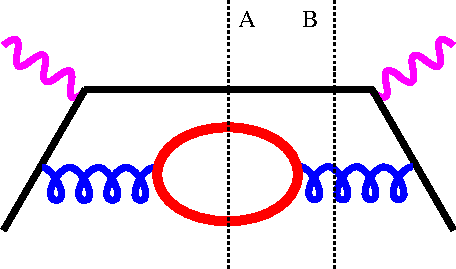
\includegraphics[width=0.45\textwidth]{pics/fred/feyngraph}
\caption{A higher order Feynman graph illustrating the difficulty in defining
  a ``fully inclusive'' $F_{2}^{charm}$.
 A light quark ($q$)
 scatters from a vector boson ($V$) with 
 a $c\bar{c}$ in the internal loop.
 If we cut the amplitude at  ``A''
we have charm in the final state and this must be included in $F_{2}^{charm}$.
If we cut the amplitude with cut ``B'' there is no charm in the
final state, but this process is required to cancel the divergences.
Additionally, since this diagram contributes to the beta function,
this highlights the complications of using an $\alpha_{S}$ and hard
scattering $\hat{\sigma}$ with differing $N_{\rm eff}$. \label{fig:bubble}}
\end{figure}

Such difficulties of defining a \textit{``fully inclusive''} $F_{2}^{c}$
are not unique to the VFNS, and also are encountered in the FFNS.
This is succinctly illustrated in Fig.~\ref{fig:bubble} which shows
a higher-order DIS process with a quark--anti-quark loop. Let us
compute this diagram in a 3-flavor FFNS where the internal loop is
a $c\bar{c}$-pair, and the external quark is a light \mbox{$\{u,d,s\}$}.
If the final-state is represented by Cut-A, then we have charm quarks
in the final state, and this should be included in $F_{2}^{c}$. 

However, if we instead use Cut-B as the final state, there is no charm
in the final state, so this should not be included in $F_{2}^{c}$.
{[}More precisely, when we renormalize the charm loop with zero-momentum
subtraction, this contribution effectively decouples.{]} Thus, the
contribution from Cut-A will be included in $F_{2}^{c}$, but the
contribution from Cut-B will not. 


If we had included the contributions for both Cut-A and Cut-B, the
total would be free of divergences. The QED analog of this is the
well known Block-Nordsieck theorem,\cite{Bloch:1937pw} and the QCD
extensions were performed by Libby and Sterman.\cite{Libby:1978bx,Libby:1978nr}
For example, the bubble diagram of Fig.~\ref{fig:bubble} is encountered
in the $F_{2}^{c}$ heavy quark calculations of Refs.~\cite{Chuvakin:1999nx,Chuvakin:2000jm};
here, an additional scale $\Delta$ must be introduced to cut on the
invariant mass of the internal quark--anti-quark pair and regulate
the singularities. 



\xsec{The running $\alpha_{S}$ in the FFNS:}
%
The bubble diagram of Fig.~\ref{fig:bubble} also highlights the
difficulty of using a $N_{\rm eff}=3$ FFNS with an $N_{\rm eff}=4$ flavor
running $\alpha_{S}(\mu)$. In a $N_{\rm eff}=3$ FFNS, internal $c\bar{c}$
loops decouple from the theory and are not included in the calculation;
however, the $N_{\rm eff}=4$ $\beta$-function requires precisely these
$c\bar{c}$ loop contributions.\footnote{Note; this deficiency can in principle be patched order-by-order by
expanding the $\beta$-function and inserting the required terms at
each order~\cite{Napoletano:2014thesis,Bierenbaum:2009zt,Cascioli:2013era}. } Once again, we cannot unambiguously divide the inclusive $F_{2}$
into separate ``light'' and ``heavy'' quantities. 



\xsec{Extensions to bottom and top:}
%
While we have used the charm quark to illustrate these features, the
same properties can, in principle, be applied to both the bottom and
top quark.\footnote{Additionally, Collins specifically addressed the case of multiple
heavy quarks which can allow for both charm and bottom in a unified
framework; in contrast to some incorrect claims in the literature,
there is no difficulty including multiple heavy quarks. (C.f, Ref.~\cite{Collins:1998rz},
Sec.~IX.)} For the case of the bottom quark, the larger mass $m_{b}$ yields
a smaller $\alpha_{s}(\mu)$ for $\mu\sim m_{b}$ and the evolution
of $f_{b}(x,\mu)$ is thus reduced; nevertheless, for large scale
processes (such as the LHC) we often find it convenient to make use
of $f_{b}(x,\mu)$ and treat the 5-flavors on an equal footing. 
%
For the case of the top quark, the very large
mass $m_{t}$ yields a much smaller $\alpha_{s}(\mu)$  for $\mu\sim m_{t}$  and the evolution
of $f_{t}(x,\mu)$ is comparatively reduced.




\subsection*{Summary }

To properly define an $F_{2}^{c}$ at all orders, we must be careful
to match the theoretical quantity to what is actually measured experimentally.
This is more complex than simply asking for the portion of $F_{2}$
which has charm in the final state, and is an issue for both the FFNS
and VFNS. The experimental $F_{2}^{c}$ is a differential cross section
for producing a charm meson in a fiducial region; this physical observable
is singularity-free and $\mu$-independent. 

We can compute in the FFNS, but in the large energy limit, we encounter
$\ln(Q^{2}/m_{c}^{2})$ divergences and this, in part, contributes
to the observed differences at large $Q$ scales. 

The VFNS includes the charm quark as an active parton for $\mu$ scales
above a matching scale $\mu_{c}$. For large $Q$ scales, the mass
singularities of NLO and SUB will cancel to yield a result free of
divergences. For scales $\mu\sim m_{c}$, cancellation between the
LO and SUB contributions ensures minimal $\mu$ dependence; however,
as this can be delicate to implement numerically, we have the option
of displacing the matching scale $\mu_{c}$ to a larger scale where
the cancellation is more stable.\cite{Bertone:2017ehk,Bertone:2018ids}


%\subsection*{Acknowledgements}
%Thanks to:
%John Collins, Ted Rogers, George Sterman, Ingo Schienbein, Aleksander Kusina

%\bibliographystyle{unsrt}
%\bibliography{fred}

%\end{document}

%%%%%%%%%%%%%%%%%%%%%%%%%%%%%%%%%%%%%%%%%


\bibliographystyle{spphys}
\bibliography{c_cpaper}

\end{document}
